\chapter[Some but not all disjunctions escape infelicity: oddness, incrementality, and scalarity]{Some but not all disjunctions escape infelicity: oddness, incrementality, and scalarity\footnotemark}\label{chap:scalarity}
\footnotetext{This Chapter includes theoretical points already made in \textcitetoappear{HenotMortier2024c} and \textcitetoappear{HenotMortier2025b}. I would like to thank the audiences and/or reviewers of the Harvard Language \& Cognition Talk Series, the 2024 HeimFest at MIT, the 2024 Amsterdam Colloquium and SALT35, in particular Jonathan Bobaljik, Ivano Ciardelli, Alexandre Cremers, Kate Davidson, Lisa Hofmann, Manfred Krifka, Jesse Snedecker, Benjamin Spector, for questions, datapoints and suggestions regarding earlier iterations of these reflections. I also thank my colleagues Omri Doron, Nina Haslinger, and Jad Wehbe for helpful discussions.}

\begin{flushright}
	\textit{To the back to the front to the back}\\
	\textit{To the back to the front to the back back}\\
	\textit{To the back to the front to the back}\\
	\textit{Back to the front back back to the front}\\
	\vspace{2mm}
	E-Phoria, D. Substance and Jin, Dlya Tebya
\end{flushright}
This Chapter focuses on Hurford Disjunctions
featuring entailing \textit{scalar} items, like \textit{some} and \textit{all} (\citenp{Gazdar1979}; \citenp{Singh2008a};\citenp{Singh2008b};\citenp{Fox2018a} i.a.). It explores how such constructions interact with (c)overt exhaustification. First, we will introduce scalar Hurford Disjunctions, along with an experimental assessment of the ordering asymmetry they arguably display. Second, we will propose a new account of the observed asymmetry, which unlike previous accounts, directly recycles independent assumptions about the nature of (c)overt exhaustification and constraints on question answering. 

\section{The challenge of scalar Hurford Disjunctions}\label{sec7:asym-exp}

\subsection{Introducing scalar Hurford Disjunctions}
Recall that Hurford Disjunctions (henceforth \textbf{HD}s, \citenp{Hurford1974}), already introduced in Chapter \ref{chap:hurford-disj}, and exemplified in (\ref{ex7:hd}), appear infelicitous. \citeauthor{Hurford1974} famously attributed this infelicity to the fact that such disjunctions involve contextually entailing disjuncts -- a constraint subsequently dubbed ``\citeauthor{Hurford1974}'s Constraint''. For simplicity, we will adopt this view in this Section.\footnote{For an overview of several more explanatory approaches to HDs, see Chapter \ref{chap:hurford-disj}, Section \ref{sec5:previous-accounts}.} In (\ref{ex7:hd}), infelicity arises regardless of the linear order of the disjuncts -- weak-to-strong (\ref{ex7:hd-ws}), or strong-to-weak (\ref{ex7:hd-sw}). 


\begin{exe}
	\ex\label{ex7:hd}
	\begin{xlist}
		\ex[\#] {SALT35 will take place in the United States or Massachusetts. \hfill \p{} $\vee$ \pplus}\label{ex7:hd-ws}
		\ex[\#] {SALT35 will take place in Massachusetts or the United States. \hfill \pplus{} $\vee$ \p}\label{ex7:hd-sw}
	\end{xlist}
\end{exe}


Interestingly, not all disjunctions apparently violating \citeauthor{Hurford1974}'s Constraint are infelicitous. \textcite{Gazdar1979} observed that HDs can become felicitous if the disjuncts are the same \textit{modulo} scalemates, like $\langle s, s^+ \rangle = \langle \textit{some}, \textit{all} \rangle$. This is exemplified in (\ref{ex7:shd-ws0}).


\begin{exe}
	\ex[] {Jo read some or all of the books. \hfill \s{} $\vee$ \splus}\label{ex7:shd-ws0}
\end{exe}

\citeauthor{Singh2008}, (\citeyear{Singh2008a}a, \citeyear{Singh2008b}b) later observed that this apparent obviation of \citeauthor{Hurford1974}'s Constraint is actually dependent on the order of the two disjuncts. If the order of the two disjuncts is reversed, as in (\ref{ex7:shd-sw}), infelicity tends to remain. We will call the two HDs in (\ref{ex7:shd}), \textbf{bare scalar HDs} (or simply \textbf{scalar HDs}). Descriptively, it seems that bare scalar HDs can be rescued from infelicity, only if the weaker disjunct precedes the stronger one.


\begin{exe}
	\ex\label{ex7:shd}
	\begin{xlist}
		\ex[] {Jo read some or all of the books. \hfill \s{} $\vee$ \splus}\label{ex7:shd-ws}
		\ex[??] {Jo read all or some of the books. \hfill \splus{} $\vee$ \s}\label{ex7:shd-sw}
	\end{xlist}
\end{exe}

Additionally, \citeauthor{Singh2008} noticed that bare scalar HDs can be overtly rescued by inserting \textit{only} within the weaker disjunct. This is illustrated in (\ref{ex7:shdo}).

\begin{exe}
	\ex\label{ex7:shdo}
	\begin{xlist}
		\ex[?] {Jo read only some or all of the books. \hfill $O(\s)\vee\splus$}\label{ex7:shdo-ws}
		\ex[] {Jo read all or only some of the books. \hfill $\splus\vee O(\s)$}\label{ex7:shdo-sw}
	\end{xlist}
\end{exe}


At a rough level of analysis, \textit{only} strengthens the weaker disjunct to contradict the stronger one: for instance, a sentence like \textit{Jo read only some of the books} (first disjunct of (\ref{ex7:shdo-ws})), typically asserts that \textit{Jo did not read all of the books} (i.e. the negation of (\ref{ex7:shdo-ws})'s second disjunct). The same can be said of (\ref{ex7:shdo-sw}), reversing the roles of the two disjuncts. So, the sentences in (\ref{ex7:shdo}) can be argued to escape \citeauthor{Hurford1974}'s Constraint, thanks to \textit{only}. We will call scalar HDs involving an overt \textit{only} like those in (\ref{ex7:shdo}), \textbf{\textit{only}-marked HDs}.\footnote{Note that (\ref{ex7:shdo-ws}) may sound more degraded than (\ref{ex7:shdo-sw}), because it appears equivalent to its bare variant without \textit{only}, (\ref{ex7:shd-ws}), which is (arguably) simpler, on top of being felicitous. We say ``arguably'', because we will see in a moment that even ``bare'' scalar HDs, especially those like (\ref{ex7:shd-ws}), have been argued to include some additional covert material akin to overt \textit{only}. So, at a structural level, it is maybe not exactly right to say that (\ref{ex7:shdo-ws}) is more complex than (\ref{ex7:shd-ws}). Still, (\ref{ex7:shdo-ws}) is probably more costly to produce than (\ref{ex7:shd-ws}) from a purely phonological point of view, regardless of structural complexity. This might play a minor role in the competition between the two sentences, and explain the relative oddness of (\ref{ex7:shdo-ws}).}\\



Why is the dataset formed by bare scalar HDs (\ref{ex7:shd}) and \textit{only}-marked scalar HDs (\ref{ex7:shdo}) challenging? First, because one must come up with a story explaining why bare scalar HDs like those in (\ref{ex7:shd}) are asymmetrically rescued, in a completely covert way. A prominent account of this asymmetry, as we will see, builds on the idea that (\ref{ex7:shd-ws}) can actually include a covert \textit{only} is its weaker disjunct -- while (\ref{ex7:shd-sw}) cannot. In any case, whatever mechanism covertly rescues (\ref{ex7:shd-ws}) (but not (\ref{ex7:shd-sw})), must be asymmetric. Second, and based on this insight, the challenge is to explain why \textit{only}, seen as an \textit{overt} rescuer, is \textit{not} asymmetric in terms of its rescuing ability. Section \ref{sec7:asym-account} will present a novel solution to these challenges.

But before presenting this analysis, the current Section will give it an additional \textit{raison d'être}, in experimentally assessing the putative contrast in (\ref{ex7:shd}) and the absence thereof in (\ref{ex7:shdo}). In particular, we will attempt to clarify whether the asymmetric felicity pattern displayed by bare scalar HDs is a robust fact, and if it is in fact tied to pragmatics. We will start with some basic theoretical background, outlining one prominent approach to scalar HDs like (\ref{ex7:shd}). The specifics of the particular analysis presented here will not be relevant to the experiments subsequently presented in this Section, but will help clarify its design and purpose.

\subsection{Previous approaches to bare scalar HDs}

The asymmetry in (\ref{ex7:shd}) has received several accounts (\cite{Singh2008a, Singh2008b,Fox2018a,Ippolito2019,Tomioka2021,HenotMortier2023} i.a.). Most of these accounts specifically focused on the pair in (\ref{ex7:shd}) -- leaving (\ref{ex7:shdo}) aside (\cite{Singh2008b} and \cite{Ippolito2019} being the two notable exceptions). All these accounts capitalize on the idea that (\ref{ex7:shd-ws}) can be rescued \textit{via} a local scalar implicature of the form \textit{some $\leadsto$ \textit{some but not all}}, targeting the first disjunct. This in turns makes the two disjuncts of (\ref{ex7:shd-ws}) incompatible -- allowing this sentence to satisfy \citeauthor{Hurford1974}'s Constraint. The aforementioned accounts differ in their treatment of (\ref{ex7:shd-sw})'s infelicity. Let us now briefly review how local scalar implicatures work, and how they can help in the case of (\ref{ex7:shd-ws}).\\

Local scalar implicatures are permitted by the covert operator \textit{exh}, which stands for \textit{exhaustification} (\cite{Fox2007}; \cite{Chierchia2009} i.a.). A definition of \textit{exh} is given in (\ref{ex7:exh-simple}).\footnote{This definition does not cover cases in which non-weaker alternatives are included \parencite{BarLev2017}, but is enough for our current purposes.} The \textit{exh} operator non-arbitrarily conjoins the proposition it attaches to (dubbed \textit{prejacent}), with the negation of non-weaker alternatives, while making sure the resulting strengthened meaning is maximally informative and non-contradictory. Let us unpack this definition. Ensuring the final result is non-contradictory and maximally informative, amounts to computing the set $\textsc{MaxExcl}(Q, p)$ of maximal ``candidate'' sets of alternatives whose negations can be all conjoined together with the prejacent without a contradiction. Ensuring the final result is not obtained in an arbitrary way, amounts to inferring the negation of the alternatives that belong to \textit{all} the candidate sets in $\textsc{MaxExcl}(Q, p)$. These alternatives form the set of so-called Innocently Excludable alternatives $\textsc{IE}(Q, p)$; see (\ref{ex7:ie}). Ensuring non-arbitrariness in exhaustification appears crucial when it comes to sets of alternatives to a prejacent that properly partition it. This is known as the Symmetry Problem \parencite{Kroch1972,Fox2007} and will be briefly discussed at the end of this Section, when we briefly go back to non-scalar HDs. 


\begin{exe}
	\ex {\textsc{\textbf{Exhaustification}. } Let $p$ be a proposition and let $Q$ be a set of relevant alternatives to $p$ that are at most as complex as $p$, in the sense of \textcite{Katzir2007}.\\
		The exhaustification of $p$ (prejacent) given $Q$, corresponds to $p$, conjoined with the negation of all Innocently Excludable alternatives in $Q$. In other words:\\
		\textit{exh}($Q$, $p$) = $p \wedge \bigwedge_{p' \in \textsc{IE}(Q, p)} \neg p'$.}\label{ex7:exh-simple}
	\ex {\textsc{\textbf{Innocent Exclusion}. } $p'$ is Innocently Excludable given $Q$ and $p$ ($p' \in \textsc{IE}(Q, p)$), iff $p'$ belongs to the intersection of the maximal subsets of $Q$ whose grand negation is consistent with $p$. In other words:\\
	$p' \in \textsc{IE}(Q, p) \iff p' \in \bigcap \textsc{MaxExcl}(Q, p)$\\
	Where $\textsc{MaxExcl}(Q, p) = \textsc{Max}_{\subseteq}(\lbrace Q' \subset Q. \ p \wedge \bigwedge_{p' \in Q'} \neg p' \not\vDash \bot \rbrace)$.}\label{ex7:ie}
\end{exe}



\textit{Exh} has an effect that is very close to that of overt \textit{only}. When applied to the first disjunct of (\ref{ex7:shd-ws}) for instance, it typically leads to the strengthening \textit{Jo read some but not all of the books}, which is roughly synonymous with \textit{Jo read only some of the books}. This is because \textit{some} typically has only one non-weaker alternative, namely \textit{all}; this single alternative therefore belongs to the one and only maximal candidate set of excludable alternatives, and so, is Innocently Excludable.\\

However, without additional assumptions, this theory predicts that \textit{exh} can be inserted in both (\ref{ex7:shd-ws}) and (\ref{ex7:shd-sw}). Both variants would in turn be predicted to be felicitous. This is illustrated in (\ref{ex7:shd-exh}).

\begin{exe}
	\ex\label{ex7:shd-exh}
	\begin{xlist}
		\ex[] {Jo read \textit{exh}(some) or all of the books. \hfill $\textit{exh}(\s)\vee\splus$\\
			$\equiv$ Jo read some but not all or all of the books. \hfill $(\s\wedge\neg\splus)\vee\splus$
		}\label{ex7:shd-ws-exh}
		\ex[??] {Jo read all or \textit{exh}(some) of the books. \hfill $\splus\vee\textit{exh}(\s)$\\
			$\equiv$ Jo read all or some but not all of the books. \hfill $\splus\vee (\s\wedge\neg\splus)$}\label{ex7:shd-sw-exh}
	\end{xlist}
\end{exe}

Therefore, assuming covert and local exhaustification correctly predicts the felicity of (\ref{ex7:shd-ws}), but also mispredicts the felicity of (\ref{ex7:shd-sw}). The challenge then shifts to explaining why (\ref{ex7:shd-sw}) cannot be rescued by \textit{exh} in the same way as (\ref{ex7:shd-ws}). Meaning, one must explain why \textit{exh} cannot be inserted (or at least cannot do its ``job'') in the second disjunct of (\ref{ex7:shd-sw}). \\

Although the implementations vary as we previously mentioned, the asymmetry between (\ref{ex7:shd-ws}) and (\ref{ex7:shd-sw}) ends up being cashed out as an interaction between the meaning of the first disjunct, and the licensing/timing of \textit{exh} in the second disjunct. One prominent account, due to \textcite{Fox2018a}, suggests \textit{exh} should not be applied to an expression $E$ if it turns out to be \textsc{Incrementally Weakening} (abbreviated \textbf{IW}). Very roughly, \textit{exh} is IW in a sentence if it leads to an equivalent/weaker meaning no matter how the sentence is finished. The constraint is spelled out in (\ref{ex7:economy}); (\ref{ex7:economy-incr-wk}-\ref{ex7:economy-prec}) unpack the definition. We will refer to the principle in (\ref{ex7:economy}) as \textit{exh}-\textsc{Economy} throughout the rest of this Chapter.

\begin{exe}
	\ex\label{ex7:economy} {\textsc{\textbf{Economy Condition on Exhaustification}} \parencite{Fox2018a}. Let \textit{exh}$(Q, p)$ be the exhaustification of $p$ given a set of alternatives $Q$. \textit{exh} cannot be inserted above $p$ in sentence $S$, abbreviated *$S$[\textit{exh}$(Q, p)$], if \textit{exh}$(Q, q)$ is incrementally weakening in $S$.}
	\ex\label{ex7:economy-incr-wk} {\textsc{\textbf{Incremental Weakening}}. An occurrence of \textit{exh} taking $p$ as argument is incrementally weakening in $S$ if it is globally weakening for every continuation of $S$ at point $p$.}
	\ex\label{ex7:economy-gl-wk} {\textsc{\textbf{Global Weakening}}. Let \textsc{IE}$(p, Q)$ be the set of Innocently Excludable alternatives to $p$ that belong to $Q$ (see (\ref{ex7:ie})). An occurrence of \textit{exh}$(Q, p)$ is globally weakening in a sentence S[\textit{exh}$(Q, p)$], if $S[p] \vDash S[\textit{exh}(Q, p)]$.\footnote{The more complex constraint spelled out in \textcite{Fox2018a}, is: $\exists Q'. \ \textsc{IE}(Q', p) \subset \textsc{IE}(Q, p) \wedge S[\textit{exh}(Q', p)] \vDash S[\textit{exh}(Q, p)]$. This means that there is a way to restrict the set of relevant alternatives to $p$, such that the resulting set of Innocently Excludable alternatives gets smaller, and the action of \textit{exh} in $S$ given this smaller set of Innocently Excludable alternatives, leads to a stronger meaning overall. Note that if $Q$ contains only one non-weaker alternative to the prejacent, then $Q'$ can only be the empty set, and the previous condition becomes $\textsc{IE}(\emptyset, p) \subset \textsc{IE}(Q, p) \wedge S[\textit{exh}(\emptyset, p)] \vDash S[\textit{exh}(Q, p)]$, i.e. $S[p] \vDash S[\textit{exh}(Q, p)]$; as given in the main text. This condition will be sufficient for our purposes, given that \textit{some} is taken to only have one salient alternative, namely \textit{all}.}}
	\ex\label{ex7:economy-cont} {\textsc{\textbf{Sentence Continuation}}. $S'$ is a continuation of $S$ at point $A$ if $S'$ can be derived from $S$ by replacement of constituents that follow $A$.}
	\ex\label{ex7:economy-prec} {\textsc{\textbf{Linear Subsequence}}. $Y$ follows $A$ if all the terminals of $Y$ are pronounced after those of $A$.}
\end{exe}
%
%A special case of interest is the following: if $C'$ is taken to be empty, $\textit{exh}_{C'}(A) = A$. This necessarily happens if $C$ is already a singleton, e.g. $C = \lbrace \forall \rbrace$: reducing it further to form $C'$ necessarily results in the empty set. An empty $C'$ then corresponds to the following subcase of (\ref{ex7:economy-gl-wk}): \textit{exh} is globally weakening if deleting it from the sentence altogether leads to an equivalent or stronger meaning. \textit{exh} will in turn be IW if deleting it from the sentence leads to an equivalent or weaker meaning, \textit{no matter the continuation} after the point of deletion. This gives rise to the simplified constraint in (\ref{ex7:economy-simple}).
%
%\begin{exe}
%	\ex\label{ex7:economy-simple} \textit{Economy Condition on Exhaustification (simplified version).} *$S$[\textit{exh}$_C(A)$], if \textit{exh}$_C$ is incrementally weakening in $S$.
%	\begin{xlist}
%		\ex {An occurrence of \textit{exh}$_C$ is globally weakening in a sentence S[\textit{exh}$_C(A)$] if $S[A] \vDash S[\textit{exh}_C(A)]$}
%		\ex {see (\ref{ex7:economy-incr-wk})}
%		\ex {see (\ref{ex7:economy-cont})}
%		\ex {see (\ref{ex7:economy-prec})}
%	\end{xlist}
%\end{exe}

%We focus on this subcase here, given that the most salient set of innocently excludable alternatives to \textit{some} is already a singleton ($\lbrace \forall \rbrace$), whose only strict subset ($C'$) is thus $\emptyset$.\\

Given \textit{exh-}\textsc{Economy}, the contrast in (\ref{ex7:shd}) then boils down to the fact \textit{exh} is not IW in the first disjunct of (\ref{ex7:shd-ws}) -- see the proof in (\ref{ex7:iw-hd-ws}) -- while it is in the second disjunct of (\ref{ex7:shd-sw}) -- see the proof in (\ref{ex7:iw-hd-sw}).


\begin{exe}
	\ex\label{ex7:iw-hd-scalar}
	\begin{xlist}
		\ex{\textit{exh}($\lbrace\s, \splus\rbrace$, \s) = $\s\wedge\neg\splus$ is not IW in the first disjunct of (\ref{ex7:shd-ws}).\\
			We have $S[\textit{exh}(\lbrace\s, \splus\rbrace, \s)] = \textit{exh}(\lbrace\s, \splus\rbrace, \s) \vee \splus$, and $S[\s] = \s \vee \splus$.\\
			Take $S'$ to be $\textit{exh}(\lbrace\s, \splus\rbrace, \s) \vee \bot$. $S'$ is a continuation of $S$ after \textit{exh}($\lbrace\s, \splus\rbrace$, \s), because it can be derived from $S$ by replacing its second disjunct with a contradiction. $\textit{exh}(\lbrace\s, \splus\rbrace, \s)$ is not globally weakening in $S'$:\\
			$S'[\textit{exh}(\lbrace\s, \splus\rbrace, \s)] = \textit{exh}(\lbrace\s, \splus\rbrace, \s) \vee \bot$\\
			\phantom{$S'[\textit{exh}(\lbrace\s, \splus\rbrace, \s)]$} $\equiv \textit{exh}(\lbrace\s, \splus\rbrace, \s)$\\
			\phantom{$S'[\textit{exh}(\lbrace\s, \splus\rbrace, \s)]$} $\equiv \s\wedge\neg\splus$\\
			\phantom{$S'[\textit{exh}(\lbrace\s, \splus\rbrace, \s)]$} $\not\Dashv \s \equiv \s \vee \splus \equiv S[\s]$\\
			Thus, $\textit{exh}(\lbrace\s, \splus\rbrace, \s)$ is not incrementally weakening in $S$.}\label{ex7:iw-hd-ws}
		\ex{\textit{exh}($\lbrace\s, \splus\rbrace$, \s) = $\s\wedge\neg\splus$ is IW in the second disjunct of (\ref{ex7:shd-sw}).\\
			We have $S[\textit{exh}(\lbrace\s, \splus\rbrace, \s)] = \splus \vee \textit{exh}(\lbrace\s, \splus\rbrace, \s)$, and $S[\s] = \splus \vee \s$.\\
			Let $S'$ be a continuation of $S$ after \textit{exh}($\lbrace\s, \splus\rbrace$, \s). Because $S'$ must result from the replacement of a constituent \textit{following} \textit{exh}($\lbrace\s, \splus\rbrace$, \s) in $S$, $S'$ can only be $S$. $\textit{exh}(\lbrace\s, \splus\rbrace, \s)$ is globally weakening in $S'=S$:\\
			$S'[\textit{exh}(\lbrace\s, \splus\rbrace, \s)] = \splus \vee \textit{exh}(\lbrace\s, \splus\rbrace, \s)$\\
			\phantom{$S'[\textit{exh}(\lbrace\s, \splus\rbrace, \s)]$}  $\equiv \splus \vee (\s\wedge\neg\splus)$\\
			\phantom{$S'[\textit{exh}(\lbrace\s, \splus\rbrace, \s)]$}  $\equiv \splus \vee\s$\\
			\phantom{$S'[\textit{exh}(\lbrace\s, \splus\rbrace, \s)]$}  $\equiv S[\s]$\\
			Thus, $\textit{exh}(\lbrace\s, \splus\rbrace, \s)$ is incrementally weakening in $S$.}\label{ex7:iw-hd-sw}
	\end{xlist}
\end{exe}

As a result, \textit{exh} can be inserted in the first disjunct of (\ref{ex7:shd-ws}), which breaks the entailment between the two disjuncts and correctly predicts the sentence to be felicitous. By contrast, \textit{exh} cannot be applied to the second disjunct of (\ref{ex7:shd-sw}), and the problematic entailment between disjuncts remains. This is illustrated in (\ref{ex7:shd-exh2}).


\begin{exe}
	\ex\label{ex7:shd-exh2}
	\begin{xlist}
		\ex[] {Jo read \textit{exh}(some) or all of the books. \hfill $\textit{exh}(\s)\vee\splus$\\
			$\equiv$ Jo read some but not all or all of the books. \hfill $(\s\wedge\neg\splus)\vee\splus$
		}\label{ex7:shd-ws-exh2}
		\ex[??] {Jo read all or *\textit{exh}(some) of the books. \hfill $\splus\vee\s$\\
			$\equiv$ Jo read all or some of the books. \hfill $\splus\vee \s$}\label{ex7:shd-sw-exh2}
	\end{xlist}
\end{exe}


Lastly, note that this approach does not overgenerate in the case of non-scalar HDs like those in (\ref{ex7:hd}). In particular, (\ref{ex7:hd-ws}) cannot be rescued like (\ref{ex7:shd-ws}), either because \textit{Massachusetts} is not a natural alternative to \textit{the United States} out-of-the blue (they convey different levels of granularity!), or, because \textit{Massachusetts} is not an Innocently Excludable alternative to \textit{the United States}. Let us further decompose the second option. If \textit{Massachusetts} can be considered a relevant alternative to \textit{the United States}, all other US states most likely can, too. Such alternatives properly partition the prejacent; thus negating them all together, would create a contradiction with the prejacent. However, negating any strict subset of these alternatives, would allow to maintain consistency with the prejacent. For instance, negating \textit{Massachusetts} would lead to a strengthened meaning along the lines of \textit{the United States, but not Massachusetts}. More drastically even, negating all US states but \textit{Massachusetts}, would lead to assert \textit{Massachusetts}. But notice that all of these options are arbitrary: negating any subset of the relevant alternatives, prevents us from negating other, equally legitimate alternatives. This is addressed by the concept of Innocent Exclusion, which forces Innocently Excludable alternatives to belong to \textit{all} maximal candidate sets of excludable alternatives. In the case of (\ref{ex7:hd-ws}), and considering state alternatives to \textit{the United States}, the maximal candidate sets of excludable alternatives, are made of all states, but one -- so there are $50$ such sets. The intersection of these sets, which corresponds to the set of Innocently Excludable alternatives, is predicted to be empty. Therefore, exhaustification is vacuous in (\ref{ex7:hd-ws}) (and (\ref{ex7:hd-sw}), for similar reasons). Consequently, both HDs in (\ref{ex7:hd}) are still correctly predicted to be infelicitous.\\

Though \textit{exh}-\textsc{Economy} successfully accounts for the asymmetry characterizing bare scalar HDs like those in (\ref{ex7:shd}), \textit{only}-marked HDs like those in (\ref{ex7:shdo}) remain a challenge. Specifically, one can wonder why \textit{only}, whose semantics is so close to that of \textit{exh}, is not subject to the \textsc{Economy} condition in (\ref{ex7:economy}).\footnote{The only principled account of this difference, is \textcite{Singh2008b}'s approach based on \textit{Local Maximize Presupposition!}; but as we will discuss, it comes at the cost of positing a non-standard entry for \textit{only}.} This will be addressed in a new way in Section \ref{sec7:asym-account}. Additionally, the subtleness of the contrast in (\ref{ex7:shd}), casts doubts on whether such an elaborate approach is needed in the first place.\footnote{It is still worth mentioning that the approach presented here comes with a range of good predictions, when it comes to more complex variants of (\ref{ex7:shd}) -- however characterized by equally subtle judgments -- but also beyond HDs. We do not cover all these predictions here, for reasons of space. See \textcite{Fox2018a} for a complete overview of these arguments.} The Section further motivates and presents two experiments testing the robustness and pragmatic significance of the contrast in (\ref{ex7:shd}), and of the absence thereof in (\ref{ex7:shdo}).

\section{An experimental assessment of the bare and only-marked scalar HDs}
\subsection{Motivations}
The two experiments we will present in this Section aim at assessing the validity of the judgments and contrasts in (\ref{ex7:shd}) and (\ref{ex7:shdo}). They address two main questions.

First, is the contrast between the bare scalar HDs (\ref{ex7:shd-ws}) and (\ref{ex7:shd-sw}) real and robust? This concern is supported by a small-scale corpus study performed by \textcite{Fox2018a} on the Corpus of Contemporary American English \parencite{Davies2008}. The data collected showed that, although the contrast between (\ref{ex7:shd-ws}) and (\ref{ex7:shd-sw}) was clearly a trend, infelicitous instances of the form (\ref{ex7:shd-sw}), were anyway attested, in about $12\%$ of the cases. Furthermore, this observation extended to other (less frequent) scalar pairs. Pairs like $\langle \textit{often}, \textit{always}\rangle$, were even characterized by an almost uniform distribution of the two disjunct orders -- though samples were small in size. Table \ref{tab7:fs-counts} compiles all the results originally reported by \textcite{Fox2018a}.


\begin{table}[H]
	\centering
	\begin{tabular}{lll}\toprule
		& Canonical order & Reverse order \\ \midrule
		some or all         & 396             & 53            \\
		some or many        & 7               & 0             \\
		some or most        & 8               & 1             \\
		most or all         & 164             & 152           \\
		many or all         & 14              & 2             \\
		can or must         & 1               & 0             \\
		may or must         & 0               & 0             \\
		sometimes or always & 3               & 2             \\
		sometimes or often  & 19              & 7             \\
		often or always     & 16              & 14            \\
		possible or certain & 1               & 0             \\
		might or must       & 0               & 0             \\
		allowed or required & 2               & 0             \\
		few or none         & 19              & 4             \\
		rarely or never     & 55              & 12            \\
		right or obligation & 1               & 0             \\
		good or excellent   & 79              & 34            \\
		Total               & 785             & 247         \\ \bottomrule
	\end{tabular}
	\caption{Results of the small scale corpus study conducted by \textcite{Fox2018a} on the Corpus of Contemporary American English, recording the number of occurrences of disjunctions of the form $\s \vee \splus$ (``canonical order'') and $\splus \vee \s$ (``reverse order''), for various pairs of scalemates $\langle\s, \splus\rangle$.}\label{tab7:fs-counts}
\end{table}

These numbers motivate an experimental assessment of the contrast in (\ref{ex7:shd}), beyond bare corpus frequencies. Yet, apart from \textcite{Chemla2013},\footnote{This study was presented as a poster. The full paper that subsequently came out of this presentation, \textcite{Chemla2016}, focuses on ``scalar'' tautological sentences of the form \textit{Jo read some or none of the books} instead of HDs. Both \textcite{Chemla2013} and \textcite{Chemla2016} however share the same methodology.} the robustness of the judgments reported in the above has never been systematically assessed in an experimental setting. It is additionally worth noting that \textcite{Chemla2013} was primarily interested in felicitous orderings like (\ref{ex7:shd-ws}), with the goal of better understanding the fine-grained processing signature of covert exhaustification in such sentences. So, in addition to assuming the presence of \textit{exh} (or any similar ``pragmatic'' operator) in (\ref{ex7:shd-ws}), this study was not designed to assess the validity of the \textit{contrast} between (\ref{ex7:shd-ws}) and (\ref{ex7:shd-sw}). Lastly, the effect of the overt exhaustifier \textit{only}, was not assessed.  The experiments presented in the following Sections intend to fill these gaps, and specifically, to determine what kind of pragmatic theory is sufficient to account for the ordering effect in (\ref{ex7:shd}), but also for the absence of a similar effect in the \textit{only}-marked HDs in (\ref{ex7:shdo}).\\

Now, assuming the contrast between the bare scalar HDs (\ref{ex7:shd-ws}) and (\ref{ex7:shd-sw}) is attested, the second question that our two studies attempt to address, is whether this contrast is really dependent on pragmatic factors. This concern is substantiated by multifactorial approaches to linear asymmetries in (conjoined) ``binomials'', like \textit{salt and pepper} vs. \textit{pepper and salt} \parencite{Benor2006}. It was shown that crisp ordering preferences in such binomials arise from a variety of extra-pragmatic factors, including metrical and frequency constraints. Is \textit{some or all} in (\ref{ex7:shd-ws}) preferable to \textit{all or some} in (\ref{ex7:shd-sw}), for similar reasons?\footnote{There are \textit{a priori} three arguments against this hypothesis. The first argument, is that there is no obvious metrical or frequency-based difference between \textit{some} and \textit{all}, so it is hard to see which order an analysis like \textcite{Benor2006} would predict to be the best. However, one could in turn argue that additional \textit{semantic} factors (e.g., likelihood, informativity) are at play in such pairs. The second, perhaps stronger argument, is that under a multivariate analysis of \textit{some or all} disjunctions \textit{à la} \textcite{Benor2006}, one might expect some cross-linguistic variation in the preferred ordering of \textit{some} and \textit{all}. But it does not seem to be the case (although, one could in turn argue that languages tend to assign \textit{some} and \textit{all} similar extra-pragmatic features, metrical, frequency, etc.). The third argument, is that the ordering asymmetry in (\ref{ex7:shd}) arguably disappears when such disjunctions are embedded in certain environments, for instance, under universal modals/quantifiers \parencite{Fox2018a}. This obviation of the asymmetry is unexpected under \textcite{Benor2006}'s analysis, because the features of the scalemates and their immediate environment, are not affected by embedding under universals. Of course, the robustness of the data introduced by \textcite{Fox2018a} and supporting an obviation, could also be questioned. Our experiments intend to bring more empirical arguments to the table, and clarify the division of labor between the aforementioned pragmatic and extra-pragmatic factors.} To better delineate the significance of these factors, our studies will test scalar HDs involving ``short'' disjuncts, like those in (\ref{ex7:shd}-(\ref{ex7:shdo}), but also similar HDs involving ``longer'' disjuncts, whereby scalemates are linearly separated by arbitrary linguistic material -- in our case, the complement/restrictor of the \textit{some} and \textit{all} quantifiers. ``Short'' HDs may be subject to ``binomial'' preferences \textit{à la} \textcite{Benor2006}, while their ``long'' counterparts are not expected to be. Thus, the assessment of ``short'' and ``long'' variants will help us determine if surface-level, ``binomial'' preferences constitute the only driver of the putative asymmetries in bare scalar HDs.

\subsection{Design and predictions}

We aim to assess the felicity of the sentences in (\ref{ex7:shd}) and (\ref{ex7:shdo}), repeated in respectively (\ref{ex7:shdr}) and (\ref{ex7:shdor}) below, along with their ``long'' variants, in (\ref{ex7:shdl}) and (\ref{ex7:shdlo}). In ``short'' variants, the restrictor of the quantifier (\textit{some} or \textit{all}) appears at the end of the second disjunct. In the below examples, the restrictor that is being used is \textit{of the books}. In short variants, the two quantifiers are thus ``directly'' disjoined -- at least on the surface. In the ``long'' variants, each disjunct features an overt restrictor: \textit{of the books} in the first disjunct, \textit{of them} in the second disjunct. The two quantifiers are thus less ``directly'' disjoined -- they are linearly separated by the restrictor of the first disjunct's quantifier, which constitutes arbitrary linguistic material (\textit{books} could be replaced by any other DP).

\begin{exe}
	\ex\label{ex7:shdr}{``Short'' disjuncts (\texttt{size=0}), no \textit{only} (\texttt{only=0}).}
	\begin{xlist}
		\ex[] {Jo read some or all of the books. \hfill \s{} $\vee$ \splus \hfill (\texttt{ordering=1})}\label{ex7:shdr-ws}
		\ex[??] {Jo read all or some of the books. \hfill \splus{} $\vee$ \s \hfill (\texttt{ordering=0})}\label{ex7:shdr-sw}
	\end{xlist}
	\ex\label{ex7:shdor}{``Short'' disjuncts (\texttt{size=0}), \textit{only} (\texttt{only=1}).}
	\begin{xlist}
		\ex[?] {Jo read only some or all of the books. \hfill $O(\s)\vee\splus$ \hfill (\texttt{ordering=1})}\label{ex7:shdor-ws}
		\ex[] {Jo read all or only some of the books. \hfill $\splus\vee O(\s)$ \hfill (\texttt{ordering=0})}\label{ex7:shdor-sw}
	\end{xlist}
\end{exe}
\begin{exe}
	\ex\label{ex7:shdl}{``Long'' disjuncts (\texttt{size=1}), no \textit{only} (\texttt{only=0}).}
	\begin{xlist}
		\ex[] {Jo read some of the books or all of them. \hfill \s{} $\vee$ \splus \hfill (\texttt{ordering=1})}\label{ex7:shdl-ws}
		\ex[??] {Jo read all of the books or some of them. \hfill \splus{} $\vee$ \s \hfill (\texttt{ordering=0})}\label{ex7:shdl-sw}
	\end{xlist}
	\ex\label{ex7:shdlo}{``Long'' disjuncts (\texttt{size=1}), \textit{only} (\texttt{only=1}).}
	\begin{xlist}
		\ex[?] {Jo read only some of the books or all of them. \hfill $O(\s)\vee\splus$ \hfill (\texttt{ordering=1})}\label{ex7:shdlo-ws}
		\ex[] {Jo read all of the books or only some of them. \hfill $\splus\vee O(\s)$ \hfill (\texttt{ordering=0})}\label{ex7:shdlo-sw}
	\end{xlist}
\end{exe}

In the four pairs of examples above, three factors are being manipulated: the presence or absence of \textit{only} (henceforth simply \texttt{only}), the ordering of the disjuncts (henceforth \texttt{ordering}), and their ``size'' (henceforth \texttt{size}). As previously mentioned, little emphasis has been so far put on the effect of \textit{overt} exhaustification with \textit{only} in (\ref{ex7:shdor}) and (\ref{ex7:shdlo}), and on how it differs from covert exhaustification. Potential differences between the ``short'' disjunctions in (\ref{ex7:shdr})-(\ref{ex7:shdor}) and the ``long'' disjunctions in (\ref{ex7:shdl})-(\ref{ex7:shdlo}) were also overlooked. Experiment $1$ assesses the absolute felicity ratings of the above sentences, while Experiment $2$ assesses the existence of an \texttt{ordering} preference between the a. and b. examples in each pair.\\

There are two (non-exclusive) hypotheses to consider when it comes to the sentences in (\ref{ex7:shdr}-\ref{ex7:shdor}) and (\ref{ex7:shdl}-\ref{ex7:shdlo}). The first hypothesis builds on \textcite{Fox2007,Chierchia2009} and assumes that the bare scalar HDs in (\ref{ex7:shdr}) and (\ref{ex7:shdl}) can be covertly and locally exhaustified. This hypothesis can be divided into two mutually exclusive subcases, that we call Case A and Case B.

In Case A, covert exhaustification is possible and incrementally unconstrained -- in other words, \textit{exh}-\textsc{Economy} (or any constraint with the same general effect) is not taken to be real. Under that view, \textit{exh} should be active in the weaker disjunct of bare scalar HDs, regardless of the order of the disjuncts. This predicts that \textit{exh} should be able to rescue \textit{both} orderings of the bare scalar HDs in (\ref{ex7:shdr}) and (\ref{ex7:shdl}). The \textit{only}-marked counterparts of these sentences, should also be quite felicitous, though perhaps slightly more degraded, due to being seemingly more complex than their \textit{only}-less counterparts. This is summarized in (\ref{ex7:hyp-atb}), and graphically schematized by the plots in Figure \ref{fig7:predictions-exh-atb}.
\begin{exe}
	\ex {\textbf{\textsc{Hypothesis 1.A.}} if covert and local exhaustification is real and incrementally unconstrained, we may expect a main, small effect \texttt{only} (favoring bare scalar HDs), no effect of \texttt{ordering}, and no effect of \texttt{size}.}\label{ex7:hyp-atb}
\end{exe}
\begin{figure}[H]
	\centering
	\begin{subfigure}[t]{.32\linewidth}
		\centering
		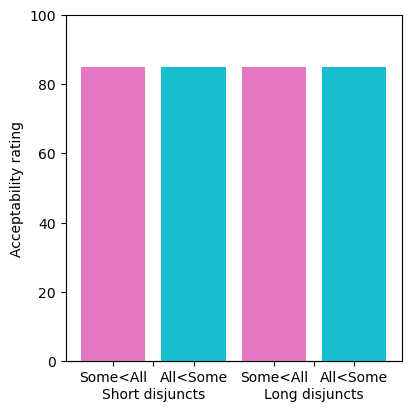
\includegraphics[width=\linewidth]{./images/pred-1a-noonly.png}
		\caption[]{Predicted ratings (Experiment $1$) for bare scalar HDs (\ref{ex7:shdr}) and (\ref{ex7:shdl}).}
	\end{subfigure}
	\hfill
	\begin{subfigure}[t]{.32\linewidth}
		\centering
		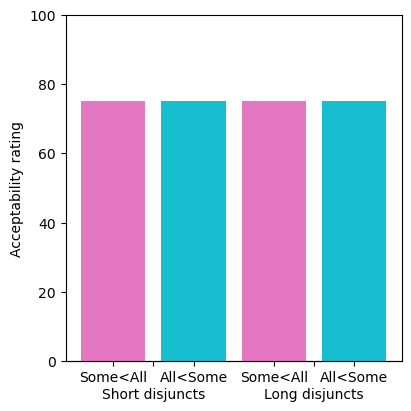
\includegraphics[width=\linewidth]{./images/pred-1a-only.png}
		\caption[]{Predicted ratings (Experiment $1$) for \textit{only}-marked HDs (\ref{ex7:shdor}) and (\ref{ex7:shdlo}).}
	\end{subfigure}
	\hfill
	\begin{subfigure}[t]{.32\linewidth}
		\centering
		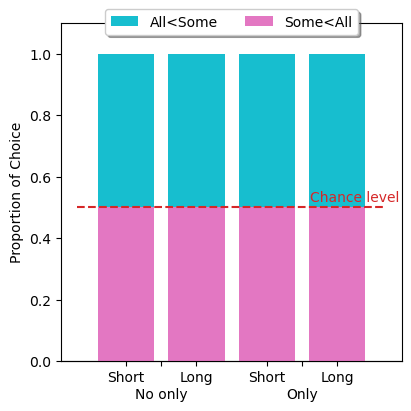
\includegraphics[width=\linewidth]{./images/pred-1a-pref.png}
		\caption[]{Predicted ordering preferences (Experiment $2$) for bare and \textit{only}-marked scalar HDs.}
	\end{subfigure}
	\caption[]{Predictions of Hypothesis 1A: covert, local exhaustification across the board, regardless of disjunct ordering.}\label{fig7:predictions-exh-atb}
\end{figure} 

In case B, covert exhaustification is possible, and incrementally constrained, for instance assuming the \textit{exh}-\textsc{Economy} constraint in (\ref{ex7:economy}). Under that view, \textit{exh} should be active in the weaker disjunct of bare scalar HDs, only when this disjunct precedes the stronger one. This predicts that \textit{exh} should be able to rescue (\ref{ex7:shdr-ws}) and (\ref{ex7:shdl-ws}), but not (\ref{ex7:shdr-sw}) or (\ref{ex7:shdl-sw}). Assuming \textit{exh}-\textsc{Economy} (or any equivalent constraint) should not apply to overt exhaustifiers, \textit{only}-marked HDs should all be quite felicitous, though (\ref{ex7:shdor-ws}) and (\ref{ex7:shdlo-ws}) may be slightly more degraded, due to being seemingly more complex than their (predicted felicitous) bare counterparts. This is summarized in (\ref{ex7:hyp-incr}), and graphically schematized by the plots in Figure \ref{fig7:predictions-exh-incr}.

\begin{exe}
	\ex {\textbf{\textsc{Hypothesis 1.B.}} if covert and local exhaustification is real and incrementally constrained, we may expect an interaction between \texttt{only} and \texttt{ordering}. Specifically, focusing on bare HDs, we expect an effect of \texttt{ordering} favoring \textit{some} $<$ \textit{all} orders. Focusing on \textit{only}-marked HDs, we expect a (potentially small) effect of \texttt{ordering} favoring \textit{all} $<$ \textit{some} orders. No effect of \texttt{size} is expected.}\label{ex7:hyp-incr}
\end{exe}

\begin{figure}[H]
	\centering
	\begin{subfigure}[t]{.32\linewidth}
		\centering
		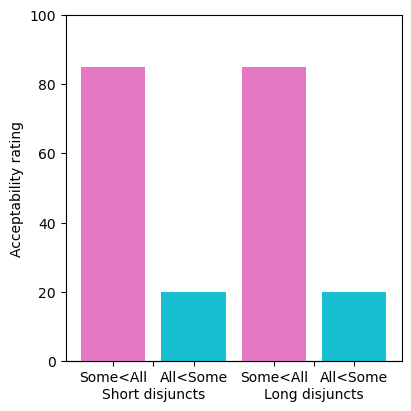
\includegraphics[width=\linewidth]{./images/pred-1b-noonly.png}
		\caption[]{Predicted ratings (Experiment $1$) for bare scalar HDs (\ref{ex7:shdr}) and (\ref{ex7:shdl}).}
	\end{subfigure}
	\hfill
	\begin{subfigure}[t]{.32\linewidth}
		\centering
		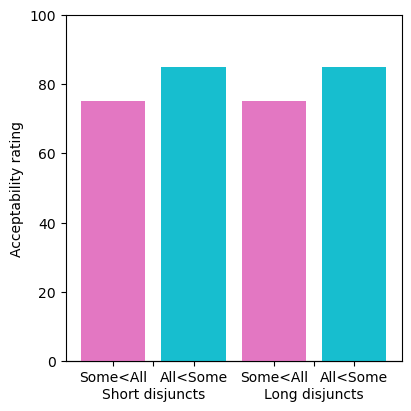
\includegraphics[width=\linewidth]{./images/pred-1b-only.png}
		\caption[]{Predicted ratings (Experiment $1$) for \textit{only}-marked HDs (\ref{ex7:shdor}) and (\ref{ex7:shdlo}).}
	\end{subfigure}
	\hfill
	\begin{subfigure}[t]{.32\linewidth}
		\centering
		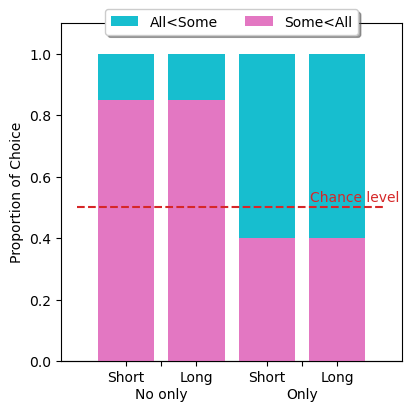
\includegraphics[width=\linewidth]{./images/pred-1b-pref.png}
		\caption[]{Predicted ordering preferences (Experiment $2$) for bare and \textit{only}-marked scalar HDs.}
	\end{subfigure}
	\caption[]{Predictions of Hypothesis 1B: covert, local, incremental exhaustification.}\label{fig7:predictions-exh-incr}
\end{figure} 


The second main hypothesis, is inspired by \textcite{Benor2006}'s findings in the domain of conjunction, and takes that the ``disjunctive binomial'' \textit{some or all} is preferred to \textit{all or some} for reasons independent of pragmatics. This hypothesis does not reject \citeauthor{Hurford1974}'s Constraint (or any specific implementation thereof), so disjunctions featuring entailing disjuncts, should in principle be deemed deviant. Rather, we understand it as being active on top of \citeauthor{Hurford1974}'s Constraint, so that it can sometimes obviate it by ``boosting'' the felicity of certain collocations, like \textit{some or all}. Under that view, (\ref{ex7:shdr-ws}) should be rescued from infelicity, since it features the favored binomial \textit{some or all}, while (\ref{ex7:shdr-sw}) should be degraded, since it features the disfavored binomial \textit{all or some}. However, such an asymmetry is not expected if the disjuncts are made ``longer'' and as such, feature additional, arbitrary linguistic material between the components of the target binomials. This implies that both ordering of the ``long'' bare scalar HDs in (\ref{ex7:shdl-ws}) and (\ref{ex7:shdl-sw}) should be degraded, due to unrescuable violations of \citeauthor{Hurford1974}'s Constraint. All \textit{only}-marked scalar HDs should be quite felicitous regardless of the occurrence of the target binomials, simply because \textit{only} rescues these sentence from a violation of \citeauthor{Hurford1974}'s Constraint. (\ref{ex7:shdor-ws}) however, may be slightly more degraded due to being seemingly more complex than its (felicitous) counterpart without \textit{only}.\footnote{This is debatable and depends on what kind of parse one wants to assign to (\ref{ex7:shdr-ws}) under that particular hypothesis. If \textit{some or all} is seen as one ``frozen'' quantifier, (\ref{ex7:shdor-ws}) and (\ref{ex7:shdr-ws}) may end being incomparable in terms of complexity.} This is summarized in (\ref{ex7:hyp-freq}), and graphically schematized by the plots in Figure \ref{fig7:predictions-freq}.
\begin{exe}
	\ex {\textbf{\textsc{Hypothesis 2.}} if ordering asymmetries in scalar HDs are only driven by preferences between binomials independent of pragmatics, we expect a three-way interaction between \texttt{only}, \texttt{ordering} and \texttt{size}. Specifically, focusing on ``long'' HDs, we expect an effect of \texttt{only} favoring \textit{only}-marked HDs, but no effect \texttt{ordering}. Focusing on ``short'' HDs, an interaction between \texttt{only} and \texttt{ordering} is expected.}\label{ex7:hyp-freq}
\end{exe}
\begin{figure}[H]
	\centering
	\begin{subfigure}[t]{.32\linewidth}
		\centering
		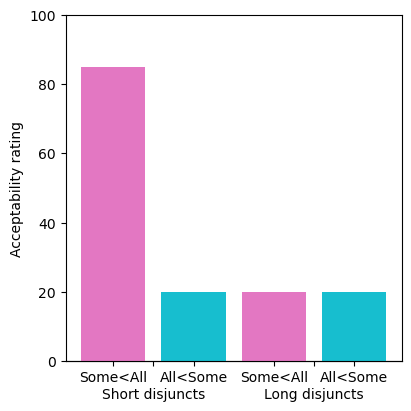
\includegraphics[width=\linewidth]{./images/pred-2-noonly.png}
		\caption[]{Predicted ratings (Experiment $1$) for bare scalar HDs (\ref{ex7:shdr}) and (\ref{ex7:shdl}).}
	\end{subfigure}
	\hfill
	\begin{subfigure}[t]{.32\linewidth}
		\centering
		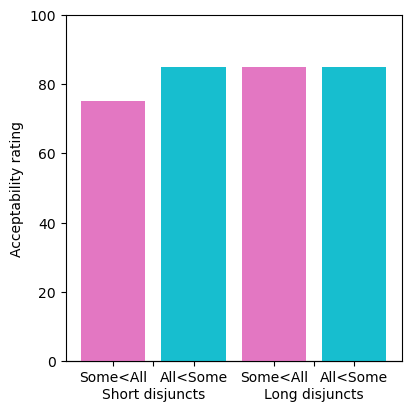
\includegraphics[width=\linewidth]{./images/pred-2-only.png}
		\caption[]{Predicted ratings (Experiment $1$) for \textit{only}-marked HDs (\ref{ex7:shdor}) and (\ref{ex7:shdlo}).}
	\end{subfigure}
	\hfill
	\begin{subfigure}[t]{.32\linewidth}
		\centering
		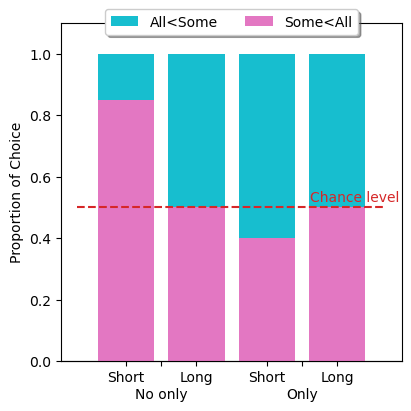
\includegraphics[width=\linewidth]{./images/pred-2-pref.png}
		\caption[]{Predicted ordering preferences (Experiment $2$) for bare and \textit{only}-marked scalar HDs.}
	\end{subfigure}
	\caption[]{Predictions of Hypothesis 2: no \textit{exh}, specific ``disjunctive binomials'' escape \citeauthor{Hurford1974}'s Constraint.}\label{fig7:predictions-freq}
\end{figure} 

We previously pointed out that Hypotheses 1 and 2 are not mutually exclusive. What would be expected if these hypotheses were both true at the same time? The are two subcases: either Hypotheses 1.A and 2 hold, or Hypotheses 1.B and 2 hold. In the former case, \textit{exh} can rescue all bare scalar HDs (Hypothesis 1.A), but those which display the \textit{all or some} binomial should be independently disfavored (Hypothesis 2), Given this, we expect the bare scalar HDs in (\ref{ex7:shdr-ws}) to be felicitous, because Hypotheses 1.A and 2 agree on this case. We also expect ``long'' bare scalar HDs to be felicitous, because Hypothesis 1.A allows these sentences to be rescued by \textit{exh}. As for the ``short'' bare scalar HD (\ref{ex7:shdr-sw}), Hypotheses 1.A and 2 make contradictory predictions: Hypothesis 1.A allows \textit{exh} to rescue this sentence, while Hypothesis 2 predicts its \textit{all or some} binomial to lead to infelicity. As a result, we expect this particular sentence to be rated lower than its other bare variants. Consequently, all \textit{only}-marked HDs should be quite felicitous, though (\ref{ex7:shdor-sw}) may be rated slightly higher, since its bare counterpart is expected to be degraded. 

\begin{exe}
	\ex {\textbf{\textsc{Hypothesis 1.A+2.}} under a mix of Hypotheses 1.A and 2, we expect a three-way interaction between \texttt{only}, \texttt{ordering}, and \texttt{size}. Focusing on ``long'' HDs, an effect of \texttt{only}, but no effect of \texttt{ordering} is expected. Focusing on ``short'' HDs, an interaction between \texttt{only} and \texttt{ordering} is expected.}\label{ex7:hyp-atb-freq}
\end{exe}

The effect structure predicted in (\ref{ex7:hyp-atb-freq}) is the same as the one predicted under Hypothesis 2 only (see (\ref{ex7:hyp-freq})); the main difference being that the felicity of ``long'' bare scalar HDs is boosted by the possibility of \textit{exh}. This is graphically schematized by the plots in Figure \ref{fig7:predictions-exh-atb-freq}.


\begin{figure}[H]
	\centering
	\begin{subfigure}[t]{.3\linewidth}
		\centering
		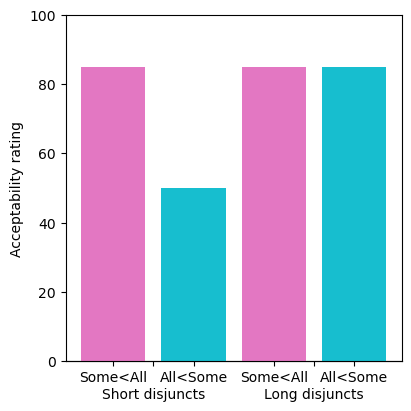
\includegraphics[width=\linewidth]{./images/pred-1a+2-noonly.png}
		\caption[]{Predicted ratings (Experiment $1$) for bare scalar HDs (\ref{ex7:shdr}) and (\ref{ex7:shdl}).}
	\end{subfigure}
	\hfill
	\begin{subfigure}[t]{.3\linewidth}
		\centering
		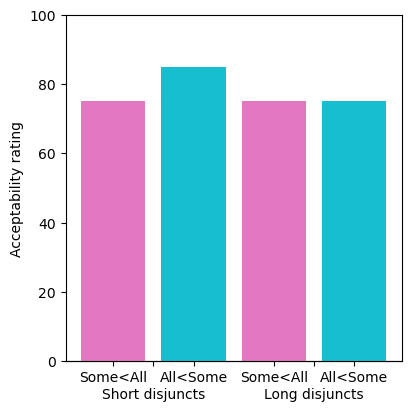
\includegraphics[width=\linewidth]{./images/pred-1a+2-only.png}
		\caption[]{Predicted ratings (Experiment $1$) for \textit{only}-marked HDs (\ref{ex7:shdor}) and (\ref{ex7:shdlo}).}
	\end{subfigure}
	\hfill
	\begin{subfigure}[t]{.3\linewidth}
		\centering
		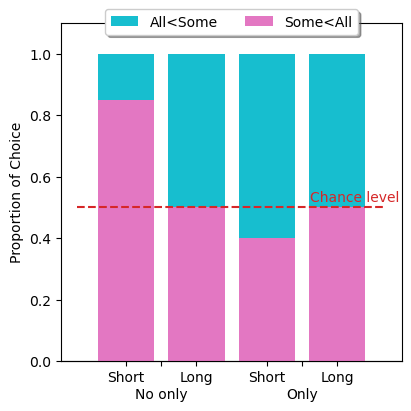
\includegraphics[width=\linewidth]{./images/pred-2-pref.png}
		\caption[]{Predicted ordering preferences (Experiment $2$) for bare and \textit{only}-marked HDs.}
	\end{subfigure}
	\caption[]{Predictions of Hypotheses 1A+2: covert, local exhaustification across the board and specific ``disjunctive binomials'' escape \citeauthor{Hurford1974}'s Constraint.}\label{fig7:predictions-exh-atb-freq}
\end{figure} 

In case Hypotheses 1.B and 2 hold together, \textit{exh} can only rescue bare scalar HDs whose first disjunct is the weaker one (Hypothesis 1.B), additionally, HDs featuring the binomial \textit{all or some}, should be disfavored (Hypothesis 2). Given this, we expect the bare scalar HDs in (\ref{ex7:shdr-ws}) and (\ref{ex7:shdl-ws}) to be felicitous, because both sentences can be rescued by incremental \textit{exh} according to Hypothesis 1.B, without contradicting Hypothesis 2. The bare scalar HDs in (\ref{ex7:shdr-sw}) and (\ref{ex7:shdl-sw}) on the other hand, are predicted independently by both hypotheses to be infelicitous. Consequently, we expect all \textit{only}-marked HDs to be quite felicitous, though (\ref{ex7:shdr-ws}) and (\ref{ex7:shdl-ws}) may be slightly more degraded, by competition with their felicitous bare counterparts. In brief, under a mix of Hypotheses 1.B and 2, we expect the same pattern as under Hypothesis 1.B alone; see (\ref{ex7:hyp-incr-freq}).

\begin{exe}
	\ex {\textbf{\textsc{Hypothesis 1.B+2.}} if covert and local exhaustification is real and incrementally constrained, we may expect an interaction between \texttt{only} and \texttt{ordering}. Specifically, focusing on bare HDs, we expect an effect of \texttt{ordering} favoring \textit{some} $<$ \textit{all} orders. Focusing on \textit{only}-marked HDs, we expect a potentially small effect of \texttt{ordering} favoring \textit{all} $<$ \textit{some} orders. No effect of \texttt{size} is expected.}\label{ex7:hyp-incr-freq}
\end{exe}

This is graphically schematized by the plots in Figure \ref{fig7:predictions-exh-incr-freq} below.
\begin{figure}[H]
	\centering
	\begin{subfigure}[t]{.3\linewidth}
		\centering
		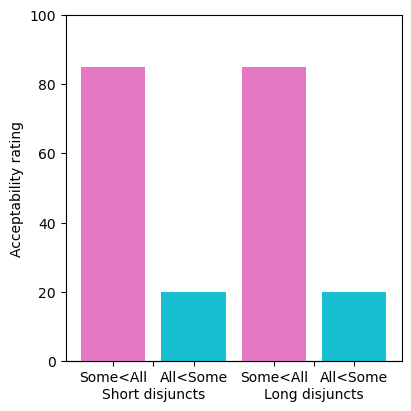
\includegraphics[width=\linewidth]{./images/pred-1b+2-noonly.png}
		\caption[]{Predicted ratings (Experiment $1$) for bare scalar HDs (\ref{ex7:shdr}) and (\ref{ex7:shdl}).}
	\end{subfigure}
	\hfill
	\begin{subfigure}[t]{.3\linewidth}
		\centering
		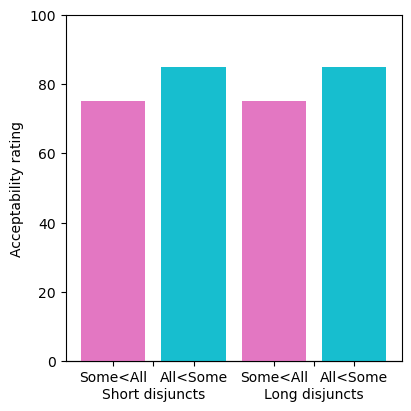
\includegraphics[width=\linewidth]{./images/pred-1b+2-only.png}
		\caption[]{Predicted ratings (Experiment $1$) for \textit{only}-marked HDs (\ref{ex7:shdor}) and (\ref{ex7:shdlo}).}
	\end{subfigure}
	\hfill
	\begin{subfigure}[t]{.3\linewidth}
		\centering
		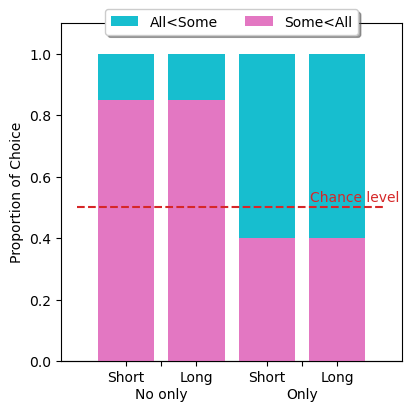
\includegraphics[width=\linewidth]{./images/pred-1b-pref.png}
		\caption[]{Predicted ordering preferences (Experiment $2$) for bare and \textit{only}-marked HDs.}
	\end{subfigure}
	\caption[]{Predictions of Hypotheses 1B+2: covert, local, incremental exhaustification and specific ``disjunctive binomials'' escape \citeauthor{Hurford1974}'s Constraint.}\label{fig7:predictions-exh-incr-freq}
\end{figure} 



Table \ref{tab7:pred-summary} summarizes the predictions of Hypotheses 1 and/or 2. In particular, it outlines the ``meta''-prediction that, if \textit{exh} is present and incremental (Hypothesis 1.B), then the predictions are not affected by the (in)validity the extra-pragmatic Hypothesis 2. Put differently, the predictions of Hypothesis 1.B alone, and of a mix of 1.B and 2, are the same. If \textit{exh} is present and \textit{not} incremental however, the predictions may follow two possible patterns. Therefore, the sentences tested are well-suited to adjudicate whether pragmatic mechanisms like covert, local exhaustification take place in scalar HDs and whether they are incrementally determined, but does not really allow us to determine unequivocally whether extra-pragmatic factors play a role in such structures.

\begin{table}[H]
	\begin{tabular}{|c|l|}
		\hline
		\small
		Hypothesis & Prediction                                                                                                                                                                                                               \\ \hline
		1.A        & Small negative effect of \texttt{only}                                                                                                                                                                                            \\ \hline
		1.B        & \begin{tabular}[c]{@{}l@{}}$2$-way interaction between \texttt{only} and \texttt{ordering}\\ \hspace*{3mm}- Bare case: \textit{some} $<$ \textit{all} preferred over \textit{all} $<$ \textit{some} \\ \hspace*{3mm}- \textit{Only}-marked case:\textit{all} $<$ \textit{only some} slightly preferred over \textit{only some} $<$ \textit{all}\end{tabular}                   \\ \hline
		2          & \begin{tabular}[c]{@{}l@{}}$3$-way interaction between \texttt{only}, \texttt{ordering} and \texttt{size}\\ \hspace*{3mm}- ``Short disjuncts'': same pattern as 1.B\\ \hspace*{3mm}- ``Long disjuncts'': positive effect of \texttt{only}\end{tabular}                 \\ \hline
		1.A+2      & \begin{tabular}[c]{@{}l@{}}$3$-way interaction between \texttt{only}, \texttt{ordering} and \texttt{size}\\ \hspace*{3mm}- ``Short disjuncts'': same kind of interaction as 1.B\\ \hspace*{3mm}- ``Long disjuncts'': small negative effect of \texttt{only} as in 1.A\end{tabular} \\ \hline
		1.B+2      & $2$-way interaction between \texttt{only} and \texttt{ordering}, as in 1.B                                                                                                                                                                \\ \hline
	\end{tabular}
	\caption[]{Summary of the hypotheses.}\label{tab7:pred-summary}
\end{table}


\subsection{Experiment 1} 
\subsubsection{Participants}
A sample of $161$ participants after all exclusions was recruited on Prolific.\footnote{The sample size before exclusions was $246$. The target sample size was determined based on a simulation-based power analysis, which indicated that a sample size of $160$ participants would provide approximately $80\%$ power to detect the critical two-way interaction between \texttt{only} and \texttt{ordering} ($\alpha=.05$). Simulations were conducted using the \texttt{simr} package in R \parencite{Green2016}, based on a generalized mixed-effect model fit to pilot data. The preregistration aimed at an initial recruitment of $200$ participants; $46$ additional participant were recruited after that threshold was reached, in order to reach the target sample size of $160$ after all exclusions. This was all specified in the preregistration.} Participants were paid \$5.25 for taking part in the study. Participants were excluded based on three main criteria. First, non-native speakers of English were excluded. Participant were asked about their native language at the beginning and at the end of the survey. Second, participants could be excluded based on their performance on practice items and fillers. Failure at all $4$ practice items (despite feedback), would result in exclusion. Failure at more than $4$ filler items (out of $16$), would also result in exclusion. Success and failure for practice and fillers items were defined as follows. If the item was expected to be felicitous, a rating of $75/100$ or more was considered a success, and a rating below $75/100$, a failure. If the item was expected to be odd, a rating of $25/100$ or less was considered a success, and a rating above $25/100$, a failure. Positive or negative feedback was given to the participants according to these thresholds, for all practice items, and for infelicitous fillers. Third, participants whose responses were to homogeneous across target items were also excluded. Responses were judged too homogeneous if the \textit{set} made of their distinct values had cardinality less than $4$, i.e. participants answered all $16$ target trials using at most $3$ different scores.\footnote{This was motivated by pilot analyses, which revealed that a non-negligible portion of the participants was almost exclusively using an extreme value or midpoint of the scale. The above criterion successfully excluded that category of participants in the pilots.}  %Figure \ref{fig7:exp1-nontargets} shows the distribution of sentence ratings for practice and filler items, after exclusions.


\subsubsection{Materials, design and procedures}
We assessed the felicity of sentences of the form (\ref{ex7:shdr}), (\ref{ex7:shdor}), (\ref{ex7:shdl}), and (\ref{ex7:shdlo}), manipulating three factors in  a $2\times2\times2$ design: \texttt{only}, \texttt{ordering}, and \texttt{size}. \texttt{ordering} and \texttt{size} were manipulated within-subject, while \texttt{only} was manipulated between-subject.\footnote{The rationale behind this choice is the following: the presence of \textit{only} is expected to make its covert counterpart, \textit{exh}, very salient, and therefore, as soon as sentences featuring \textit{only}, like those in (\ref{ex7:shdor}) and (\ref{ex7:shdlo}) are presented to participants, these participants become be more likely to use, or not use, \textit{exh} in sentences like (\ref{ex7:shdr}) and  (\ref{ex7:shdl}). Said differently, if \textit{only} were within-subject, and participants were thus exposed to both bare scalar HDs and \textit{only}-marked HDs, judgments produced for the former would be inevitably influenced by judgments produced for the latter. Manipulating both \texttt{ordering} and \texttt{size} within-subject does not lead to the same kind of concern. I thank Athulya and Nadine Bade for pointing out this caveat to me.}


Felicity was assessed through a sentence rating task.\footnote{This task was preceded by a self-paced reading task used for exploratory analyses.} Participants were randomly assigned to a group (\texttt{only} or \texttt{no-only}) when entering the survey. In each trial, participants were presented with a short scenario, involving three named individuals,\footnote{Names were randomly chosen when designing the items. They were balanced in terms of gender, and picked to be sufficiently distinct from each other (different initial, at most $3$ letters in common).} that we will call A, B, and C here. Each scenario was constructed as follows. C is expected by A and B to do a certain action involving a specific set of objects. C is then made unavailable, causing to A to ask B about C's action. In the case of target trial, B answers to A a disjunctive sentence of the from (\ref{ex7:shd}) or (\ref{ex7:shdl}) (for the \texttt{no-only} group), or, (\ref{ex7:shdo}) or (\ref{ex7:shdl}) (for the \texttt{only} group). This target sentence is preceded by a statement of uncertainty of the form \textit{I'm not sure but...}, to justify the use of a disjunction. This is exemplified in Figure \ref{fig7:exp1-screen-target}, whereby A, B and C are Carolyn, Denise and Noah respectively.

\begin{figure}[H]
	\centering
	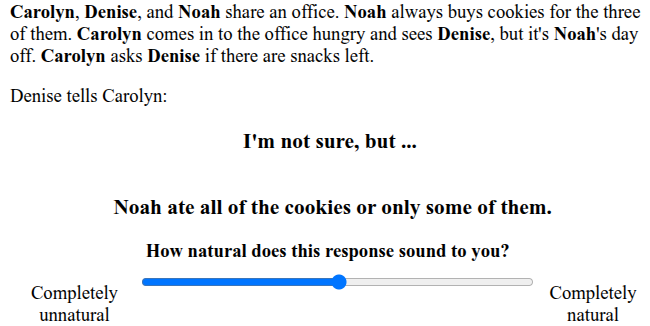
\includegraphics[width=.5\linewidth]{./images/exp1-screen-target.png}
	\caption[]{Sentence rating task (Experiment $1$). A target item from the \texttt{only} group.}\label{fig7:exp1-screen-target}
\end{figure}

In the case of filler trials, scenarios were similar, except B answers to A quantified sentences of the form (\ref{ex7:good-fillers}) or (\ref{ex7:bad-fillers}). (\ref{ex7:good-fillers}) were felicitous fillers, corresponding to simple quantified sentences devoid of a disjunctive operator. (\ref{ex7:bad-fillers}) were infelicitous fillers, corresponding to sharply redundant sentences involving the same two quantified disjuncts. (In)felicitous fillers were not preceded by a statement of uncertainty, as shown in Figure \ref{fig7:exp1-screen-fillers}.

\begin{exe}
	\ex \label{ex7:good-fillers}
	\begin{xlist}
		\ex[] {Jo read some of the books.}\label{ex7:good-filler-some}
		\ex[] {Jo read all of the books.}\label{ex7:good-filler-all}
	\end{xlist}
	\ex \label{ex7:bad-fillers}
	\begin{xlist}
		\ex[] {Jo read some or some of the books.}\label{ex7:bad-filler-some}
		\ex[] {Jo read all or all of the books.}\label{ex7:bad-filler-all}
	\end{xlist}
	
\end{exe}

\begin{figure}[H]
	\centering
	\begin{subfigure}[b]{.45\linewidth}
		\centering
		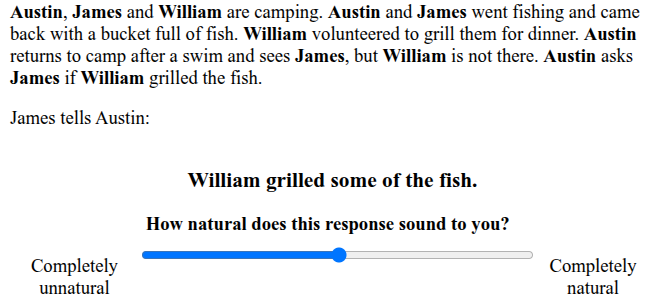
\includegraphics[width=\linewidth]{./images/exp1-screen-filler-good.png}
		\caption[]{A felicitous filler of the form (\ref{ex7:good-filler-some}).}
	\end{subfigure}
	\hfill
	\begin{subfigure}[b]{.45\linewidth}
		\centering
		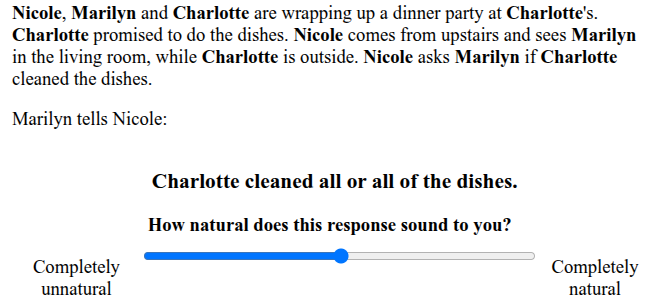
\includegraphics[width=\linewidth]{./images/exp1-screen-filler-bad.png}
		\caption[]{An infelicitous filler of the form (\ref{ex7:bad-filler-all}).}
	\end{subfigure}

	\caption[]{Sentence rating task (Experiment $1$). Filler items (shared by both groups).}\label{fig7:exp1-screen-fillers}
\end{figure}

Practice items followed the same general structure. In all cases, participants were asked to rate how natural the sentence was to them, using an unlabeled Likert scale ranging from $0$ to $100$. Participants received feedback during practice and after infelicitous fillers. Practice items, feedback messages, along with fillers and target items are described in more detail in Appendix \ref{sec7:exp1-practice-feedback}.\\

Target and filler items were organized as follows. Each participant was exposed to a total of $4$ blocks, each block containing $8$ trials ($4$ target trials and $4$ fillers). So there were $32$ test trials in total. In each block, the $4$ target trials were designed to represent all combinations of \texttt{ordering} ($2$ levels) and \texttt{size} ($2$ levels). Target trials and scenarios followed a Latin Square design, such that each group (\texttt{only}/\texttt{no-only}), was subdivided into $4$ subgroups. Across these $4$ subgroups, the Latin Square design ensured that each \texttt{ordering}-\texttt{size} combination got paired with a given scenario only once, and each particular scenario got paired with each \texttt{ordering}-\texttt{size} combination only once. Fillers followed the structure of the sentences in (\ref{ex7:good-fillers}) and (\ref{ex7:bad-fillers}). They were randomly interspersed between the target trials of each block, in such a way that (i) each block contained exactly $4$ fillers, one of each type; (ii) how the fillers got randomly inserted changed between block $1$, $2$, $3$, and $4$; (iii) how the fillers got randomly inserted for a given block (e.g. block $1$), did not change across subgroups. The full design is available for consultation on \href{https://osf.io/fn9p4}{OSF}.



%\begin{figure}[H]
%	\centering
%	\begin{subfigure}[b]{.45\linewidth}
%		\centering
%		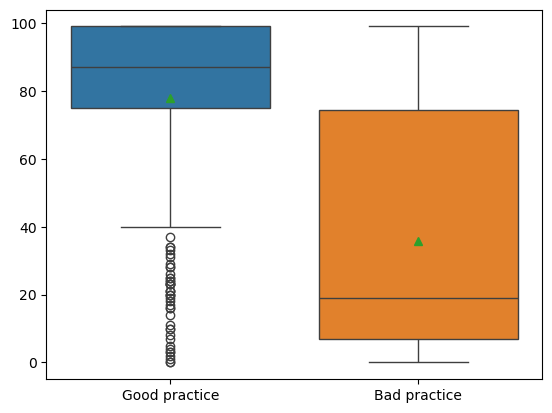
\includegraphics[width=\linewidth]{./images/exp1-practice.png}
%		\caption{Practice}
%	\end{subfigure}
%	\hfill
%	\begin{subfigure}[b]{.45\linewidth}
%		\centering
%		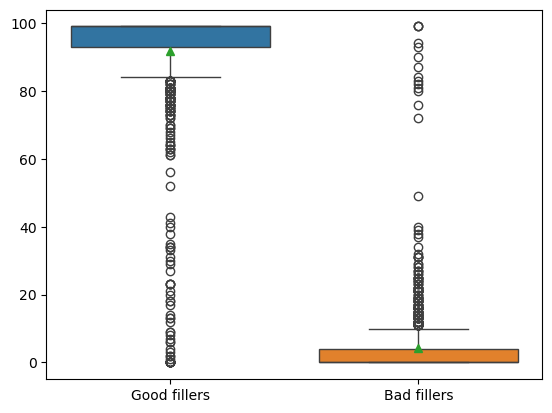
\includegraphics[width=\linewidth]{./images/exp1-fillers.png}
%		\caption{Fillers}
%	\end{subfigure}
%	\caption{Ratings for non-target items (after exclusions).}\label{fig7:exp1-nontargets}
%\end{figure}

\subsubsection{Results}
We analyzed the ratings (between $0$ and $100$) assigned by the participants to the target sentences. Ratings were modeled using a mixed effect linear regression \parencite{Bates2015,Kuznetsova2017}. The goal was to evaluate if the ratings assigned to sentences was dependent on an interaction between \texttt{only} and \texttt{ordering}. Factors were encoded according to Table \ref{tab7:factor-coding} and then sum-coded. 

\begin{table}[H]
	\centering
	\begin{tabular}{|r|r|r|ll|}
		\hline
		\texttt{size} & \texttt{only} & \texttt{ordering} & \multicolumn{2}{l|}{example sentence} \\ \hline
		0    & 0        & 0    & \multicolumn{1}{l}{} (\ref{ex7:shd-sw})  & Jo read all or some of the books.   \\ \hline
		0    & 0        & 1    & \multicolumn{1}{l}{}  (\ref{ex7:shd-ws}) & Jo read some or all of the books.  \\ \hline
		0    & 1        & 0    & \multicolumn{1}{l}{} (\ref{ex7:shdo-sw})  & Jo read all or only some of the books.  \\ \hline
		0    & 1        & 1    & \multicolumn{1}{l}{} (\ref{ex7:shdo-ws})  &  Jo read only some or all of the books.  \\ \hline
		1    & 0        & 0    & \multicolumn{1}{l}{} (\ref{ex7:shdl-sw})  &   Jo read all of the books or some of them. \\ \hline
		1    & 0        & 1    & \multicolumn{1}{l}{} (\ref{ex7:shdl-ws})  &  Jo read some of the books or all of them. \\ \hline
		1    & 1        & 0    & \multicolumn{1}{l}{} (\ref{ex7:shdlo-sw})  &  Jo read all of the books or only some of them.  \\ \hline
		1    & 1        & 1    & \multicolumn{1}{l}{} (\ref{ex7:shdlo-ws})  &  Jo read only some of the books or all of them.  \\ \hline
	\end{tabular}
	\caption{Coding of the three factors \texttt{size} ($0$=short disjuncts, $1$=long disjuncts), \texttt{only} ($0$=no \textit{only}, $1$=\textit{only}) and \texttt{ordering} ($0$=\textit{all} $<$ \textit{some}, $1$=\textit{some} $<$ \textit{all}).}\label{tab7:factor-coding}
\end{table}

 We included the maximum random effect structure supported by the data, in the form of an intercept by scenario \texttt{(1$|$scenario)}, as well as a random slope for \texttt{size} within \texttt{participant} \texttt{(size$|$participant)}. The complete syntax of the model was then $\texttt{rating} \sim \texttt{only}*\texttt{ordering} + (1|\texttt{scenario}) + (\texttt{size}|\texttt{participant})$.\\

Significance was assessed using Type III Wald $\chi^2$ tests with the \texttt{car} package in R \parencite{Fox2019}. A significant negative interaction was detected between \texttt{ordering} and \texttt{only} interaction ($\chi^2 = 7.03$; $p<.05$). This interaction was disfavoring instances of \textit{only some or all}, i.e. (\ref{ex7:shdo-ws}) and (\ref{ex7:shdlo-ws}). No significant main effects of \texttt{ordering} or \texttt{only} were detected.\\

The existence of a significant negative interaction between \texttt{ordering} and \texttt{only} goes against Hypothesis 1.A, but does not by itself allow to tease apart the other possible hypotheses, which all predict that \textit{only some or all} should be dispreferred by competition with the felicitous \textit{some or all}; and that \textit{all or only some} is not subject to the same kind of competition. Additionally, this interpretation of the interaction crucially hinges on the existence of a main effect of \texttt{ordering}, and \texttt{only}. But such effects were not detected.

The fact that \texttt{ordering} did not have a significant effect on the ratings of target sentences appears more in line with Hypothesis 1.A. The fact that \texttt{only} did not have a significant effect on the ratings either also appears more compatible with Hypothesis 1.A. The absence of these main effects is corroborated by the plots in Figure \ref{fig7:exp1-targets}, which do not show clear evidence of the expected differences in felicity. This makes the interaction between \texttt{ordering} and \texttt{only} difficult to interpret: such an interaction would make sense if any hypothesis different from Hypothesis 1.A were true; but the very absence of main effects, supports Hypothesis 1.A.


\begin{figure}[H]
	\centering
	\begin{subfigure}[b]{.45\linewidth}
		\centering
		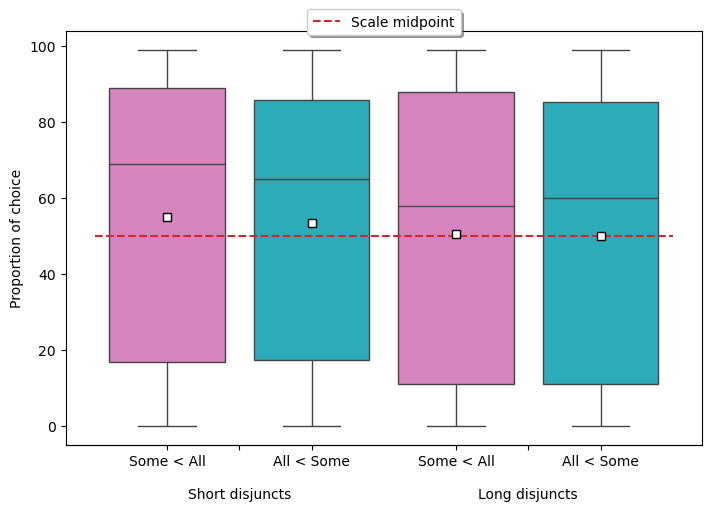
\includegraphics[width=\linewidth]{./images/exp1-target-noonly.png}
		\caption{\texttt{no-only} group.}
	\end{subfigure}
	\hfill
	\begin{subfigure}[b]{.45\linewidth}
		\centering
		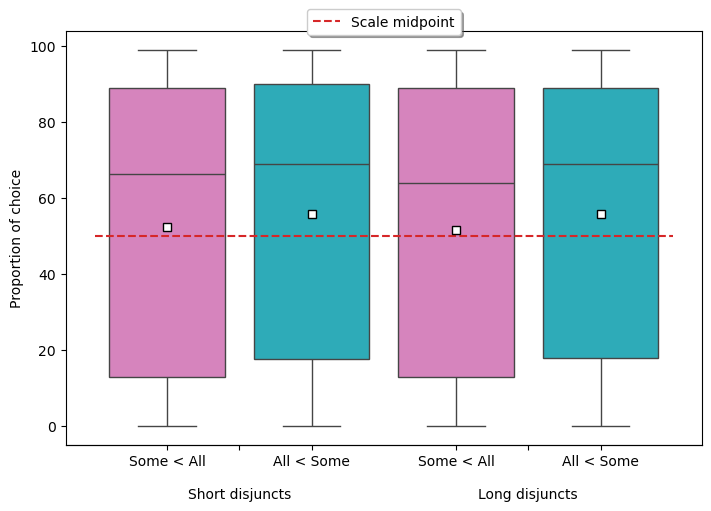
\includegraphics[width=\linewidth]{./images/exp1-target-only.png}
		\caption{\texttt{only} group.}
	\end{subfigure}
	\caption{Ratings for target items. White squares correspond to mean ratings.}\label{fig7:exp1-targets}
\end{figure}


An analysis of the participants individuals responses revealed that many participant restricted their ratings of the target sentences to a specific area of the scale: either above $50$ or below $50$, which made the distributions of sentence ratings overall bimodal. More crucially perhaps, this may indicate that participants were not reflecting about fine-grained differences between the target sentences, but instead were trying to coarsely assign each target sentence to a ``roughly good'' or ``roughly bad'' area of the scale. To neutralize this caveat, Experiment 2 adopts a perhaps simpler and more direct paradigm, using a binary selection task (for relative comparisons between sentences) instead of a Likert scale (for absolute ratings).

% todo ADD SWARMPLOTS / PARTICIPANT CLUSTERING

\subsection{Experiment 2} 


\subsubsection{Participants}
A sample of $200$ participants after all exclusions ($100$ per group, $25$ per subgroup) was recruited.\footnote{Sample size before exclusions was $200$, as well. Sample sizes pre- and post-exclusions were based on Experiment $1$.} Exclusion criteria were similar to Experiment $1$: non-native speakers of English were excluded; participants who failed at all $5$ practice items and/or at more than $4$ filler items (out of $16$), despite feedback, were excluded. This did not actually give rise to exclusions. Unlike Experiment $1$, Experiment $2$ did not have a ``homogeneity'' exclusion criterion. Instead, there were item-level exclusions based on reaction times:\footnote{I thank Kate Kinnaird for suggesting this.} trials in which participants were too fast or too slow to submit a definitive selection were discarded. $36$ (out of $7400$) trials were excluded due to short reaction times. This was including $18$ targets trials. The lower threshold was set to $1500$ millisecond between the display of the choices and the submission of a preference; it was determined empirically when testing the experiment. Additionally, $42$ trials (including $14$ targets trials) were excluded due to long reaction times. The upper threshold was set to approximately $222$ seconds, which corresponds to the mean reaction time over all trials, plus $3$ standard deviations. Both the lower and the upper threshold were defined in the preregistration.

\subsubsection{Materials, design and procedures}

For each pair of sentences in (\ref{ex7:shd}), (\ref{ex7:shdo}), (\ref{ex7:shdl}), and (\ref{ex7:shdlo}), we assessed which \texttt{ordering} was \textit{preferred} -- a binary choice. A choice favoring the \textit{some} $<$ \textit{all} \texttt{ordering} over the \textit{all} $<$ \textit{some} \texttt{ordering}, was coded as $1$, and a choice favoring the \textit{all} $<$ \textit{some} \texttt{ordering} over the \textit{some} $<$ \textit{all} \texttt{ordering}, was coded as $0$. $2$ factors were manipulated in  a $2\times2$ design: \texttt{only}, and \texttt{size}. These factors were coded just like in Experiment $1$ -- see Table \ref{tab7:factor-coding}. Similarly to Experiment $1$, \texttt{size} was manipulated within-subject, while \texttt{only} was manipulated between-subject.\\

Sentences and scenarios were the same as in Experiment 1.\footnote{Some practice items were modified, and one practice item was added. Names were changed. See Appendix.} The only difference in terms of design, was that, in each trial, two critical sentences were presented instead of one. Participants had to choose, between the two proposed sentences, which ones sounds the most natural. A sentence could be selected by clicking on it; participants could change their selection any number of times, before clicking on the ``Submit'' button, displayed as soon as a initial selection was made. Screenshots of the trials are given in Figures \ref{fig7:exp2-screen-target} and \ref{fig7:exp2-screen-fillers}.

\begin{figure}[H]
	\centering
	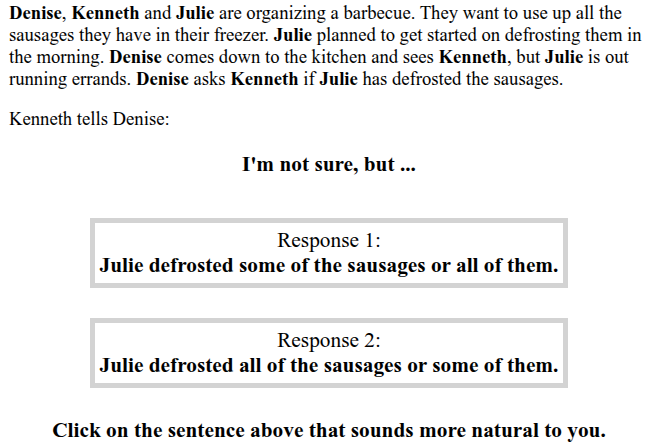
\includegraphics[width=.5\linewidth]{./images/exp2-screen-target.png}
	\caption[]{Sentence comparison task: target item (\texttt{no-only} group).}\label{fig7:exp2-screen-target}
\end{figure}

\begin{figure}[H]
	\centering
	\begin{subfigure}[b]{.45\linewidth}
		\centering
		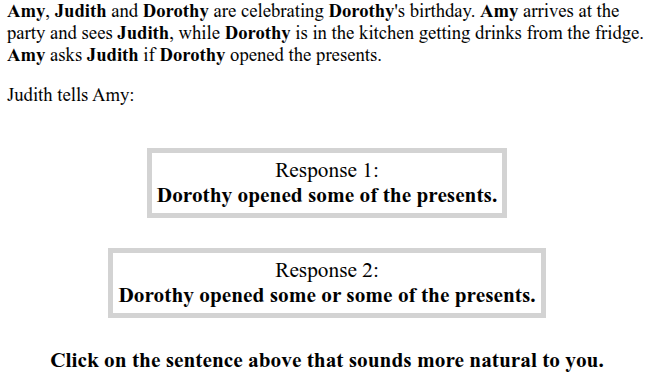
\includegraphics[width=\linewidth]{./images/exp2-screen-filler-some.png}
		\caption[]{Pairs of fillers of the form (\ref{ex7:good-filler-some})-(\ref{ex7:bad-filler-some}).}
	\end{subfigure}
	\hfill
	\begin{subfigure}[b]{.45\linewidth}
		\centering
		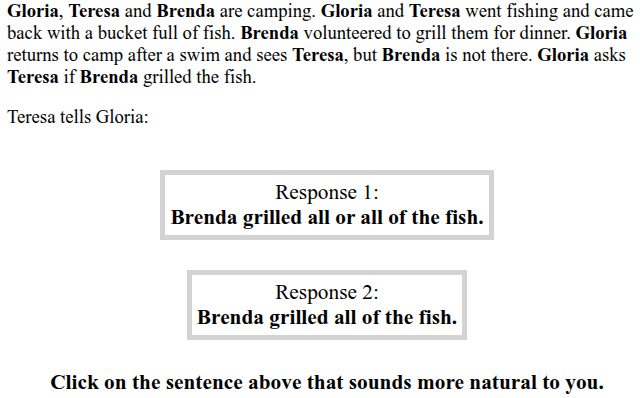
\includegraphics[width=\linewidth]{./images/exp2-screen-filler-all.png}
		\caption[]{Pairs of fillers of the form (\ref{ex7:bad-filler-all})-(\ref{ex7:good-filler-all}).}
	\end{subfigure}
	
	\caption[]{Sentence comparison task: filler items (both groups).}\label{fig7:exp2-screen-fillers}
\end{figure}


The organization of the trials varied minimally from Experiment $1$. Specifically, each trial of Experiment $1$ was modified in the following way to fit the task of Experiment $2$: the critical sentence from Experiment $1$ was treated as the first/top sentence (labeled ``Response $1$'') on screen, and its swapped-disjunct counterpart\footnote{In the case of fillers, (\ref{ex7:good-filler-some}) and (\ref{ex7:bad-filler-some}) were mutual counterparts, an so were (\ref{ex7:good-filler-all}) and (\ref{ex7:bad-filler-all}).} was added as the second/bottom sentence on screen (labeled ``Response $2$''). In other words, target trials displayed the a. and b. examples of the pairs in (\ref{ex7:shd}), (\ref{ex7:shdo}), (\ref{ex7:shdl}), and (\ref{ex7:shdlo}) side by side, for comparison. The critical pairs presented were thus only differing in terms of the \texttt{ordering} factor, leaving all other factors fixed. Since \texttt{ordering} was controlled in Experiment $1$, the modification of the display performed to construct Experiment $2$, ensured that Experiment $2$ was controlled in terms of side bias.  The full design is available for consultation on \href{https://osf.io/kn692}{OSF}.



\subsubsection{Results}

Our dependent variable, \texttt{choice}, was set to $1$ if the \textit{some} $<$ \textit{all} \texttt{ordering} was preferred over the \textit{all} $<$ \textit{some} \texttt{ordering}; and to $0$ otherwise. In case there is no preference between the two possible \texttt{orderings} of the disjuncts, the proportion of \texttt{choice} is expected to be at $50\%$. A high proportion of choice, indicates a preference for the \textit{some} $<$ \textit{all} \texttt{ordering}.\\

Figure \ref{fig7:exp2-targets} shows the proportion of \texttt{choice} for the target trials. It can be seen that the \textit{some} $<$ \textit{all} ordering is clearly preferred (in around $80\%$ of the cases) in the \texttt{no-only} group, regardless of disjunct \texttt{size}.\footnote{Fitting intercept-only models for each subgroup confirmed this. } This appears consistent with the introspective judgments in (\ref{ex7:shd}) and (\ref{ex7:shdl}), and Hypothesis 1.B(+2). Moreover, the \textit{some} $<$ \textit{all} ordering is no longer preferred -- in fact, the opposite ordering is slightly preferred -- in the \texttt{only} group.\footnote{Fitting intercept-only models for each subgroup returned a non significant negative estimate in the case of short disjuncts, and significantly negative estimate in the case of long disjuncts.} with what seems to be a small effect of disjunct \texttt{size}, increasing the preference for \textit{all} $<$ \textit{some} orderings under the long disjunct condition. Though these preference measurements do not indicate felicity \textit{per se}, they again appear consistent with the introspective judgments in (\ref{ex7:shdo}) and (\ref{ex7:shdlo}), and Hypothesis 1.B, according to which \textit{all} $<$ \textit{only some} should be slightly preferred over \textit{only some} $<$ \textit{all} due to competition with the corresponding bare scalar HDs.


%\begin{subfigure}[b]{.45\linewidth}
%	\centering
%	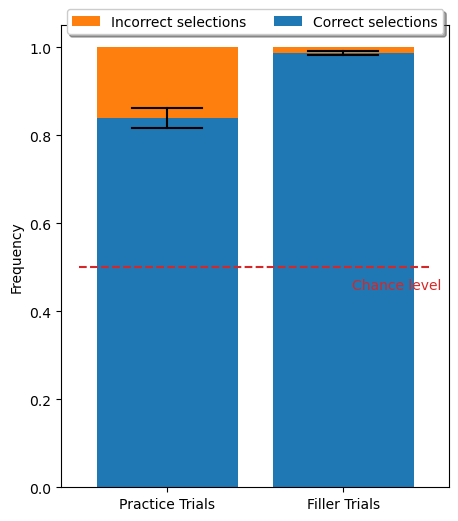
\includegraphics[height=6cm]{./images/exp2-practice-fillers.png}
%	\caption{Non-target items (practice and fillers).}\label{fig7:exp2-nontargets}
%\end{subfigure}

\begin{figure}[H]

		\centering
		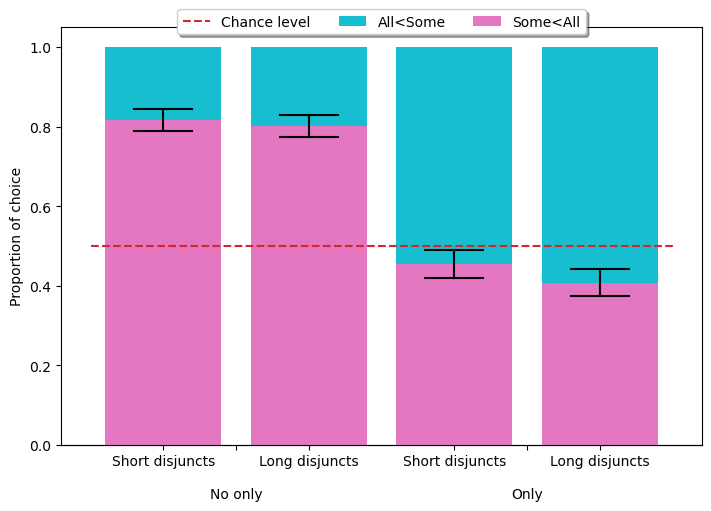
\includegraphics[width=.6\linewidth]{./images/exp2-targets.png}
		\caption{Target items (both groups).}\label{fig7:exp2-targets}
	\caption{Results of Experiment $2$ after exclusions. Error bars are $95\%$ confidence intervals.}
\end{figure}

To corroborate the trends observed in the above plots, \texttt{ordering} preferences were modeled using a mixed effect logistic regression. The goal was to confirm that the preference for the \textit{some} $<$ \textit{all} \texttt{ordering} over the \textit{all} $<$ \textit{some} \texttt{ordering} was dependent on the presence of \textit{only} -- as strongly suggested by the plots. Factors were sum-coded. We included the maximum random effect structure supported by the data, in the form of an intercept by participant (\texttt{(1$|$participant)}).\footnote{The number of optimization iterations had to be increased for the models to converge, using the option \texttt{glmerControl(optimizer = "bobyqa", optCtrl = list(maxfun = 100000))}.} The complete syntax of the model was then $\texttt{choice} \sim \texttt{only}*\texttt{size} + (1|\texttt{participant})$.\\ %should i try to add sie as slope?


Significance was assessed using Type III Wald $\chi^2$ tests with the \texttt{car} package in R \parencite{Fox2019}. 
A significant negative main effect of \texttt{only} was detected ($\chi^2 = 90.8$; $p<.05$), decreasing the preference for \textit{some} $<$ \textit{all} over \textit{all} $<$ \textit{some}, in the presence of \textit{only}.
A significant negative main effect of \texttt{size} was also detected ($\chi^2 = 5.2$; $p<.05$), decreasing the preference for \textit{some} $<$ \textit{all} over \textit{all} $<$ \textit{some}, with long as opposed to short disjuncts.\footnote{Exploratory analyses showed that this effect was driven by the \texttt{only} group -- as suggested by the plots. Fitting a model with only \texttt{size} as factor in the \texttt{no-only} group did not yield a significant main effect, while it did in the \texttt{only} group.}
Interestingly, no interaction was detected between \texttt{ordering} and \texttt{only} in this Experiment.


The main effect of \texttt{only} is in line, is again in line with Hypothesis 1.B(+2), or Hypothesis (1.A)+2. However, the existence of an effect of \texttt{size} driven by the \texttt{only} group, goes strongly against Hypothesis (1.A)+2, which predicts \texttt{size} to negatively affect the \textit{some} $<$ \textit{all} preference in the \texttt{no-only} group, and positively affect it in the \texttt{only} group. Therefore, the overall pattern rather supports Hypothesis 1.B(+2). The only unexpected effect is that of \texttt{size} in the the \texttt{no-only} group: Hypothesis 1.B(+2) does not predict such an effect.\\

Experiment $2$ strongly Hypothesis 1.B, according to which bare scalar HDs are asymmetrically rescued by a covert, local, and incremental exhaustification operator. This Experiment however, did not provide any absolute measurement of felicity or oddness, so could not help us determine if the overt exhaustifier \textit{only} equally \textit{rescues} scalar HDs. The data from Experiment $1$ however, were showing a trend in this direction.

\subsection{Interim Summary}
In this first part of the Chapter, we have introduced bare and \textit{only}-marked scalar HDs, along with an existing theoretical approach to the two-way asymmetry such structures were argued to display. We then presented two Experiments testing the significance of this asymmetry. Experiment $1$ was rather inconclusive, which we suggested may be attributed to the degree of precision the participants felt expected to provide in their ratings of the target sentences. Experiment $2$, which was built around a more direct paradigm, resulted in more interpretable data, supporting the empirical picture described in the theoretical literature. With this in mind, we proceed to propose a new account of bare and \textit{only}-marked scalar HDs. The analysis will draw from independently motivated constraints, that we will rephrase in an incremental implicit QuD framework.



\section{A novel account account of the asymmetries in scalar Hurford Disjunctions}\label{sec7:asym-account}

In this Section, we present a novel account of the oddness asymmetry displayed by bare scalar HDs, and the lack thereof in \textit{only}-marked HDs. We will refer to their short disjunct variants, repeated in (\ref{ex7:shd}) and (\ref{ex7:shdo}) below.

\begin{exe}
	\exr{ex7:shd}{Bare scalar HDs}
	\begin{xlist}
		\ex[] {Jo read some or all of the books. \hfill \s{} $\vee$ \splus}
		\ex[??] {Jo read all or some of the books. \hfill \splus{} $\vee$ \s}
	\end{xlist}
	\exr{ex7:shdo}{\textit{Only}-marked HDs}
	\begin{xlist}
		\ex[?] {Jo read only some or all of the books. \hfill $O(\s)\vee\splus$}
		\ex[] {Jo read all or only some of the books. \hfill $\splus\vee O(\s)$}
	\end{xlist}
\end{exe}

Our analysis will recycle independently motivated claims on overt and covert exhaustifiers, and constraints on question answering. The core intuition is the following: covertly exhaustifying \textit{some} in the second disjunct of a bare scalar HD like (\ref{ex7:shd-sw}) trivializes the incremental question raised by the first disjunct; while overtly exhaustifying \textit{some} using \textit{only}m as in (\ref{ex7:shdo-sw}), does not. %This intuition will be shown to extend outside of HDs, for instance, to the domain of Sobel Sequences.
We will proceed in three steps. First, we will clarify what the Qtrees for scalemate expressions involving \textit{some} and \textit{all} are predicted to be in our framework. We will also spell out what kind of Qtree can be incrementally inferred from the disjunction of \textit{some} and \textit{all}. Second, we will define how overt and covert exhaustification operators (\textit{only}, \textit{exh}) affect Qtrees, based on how they divide up the work between presupposition and assertion. Third and lastly, we will adapt an existing constraint on felicitous question answering to the current framework, and show how it can actually capture the data at stake. In the rest of this Section, we will sometimes use \textit{some} and \textit{all} as shorthands for propositions/LFs differing only in terms of these two scalemates. This will be used to talk about the two disjuncts of bare scalar HDs, for instance.

\subsection{Qtree evoked by scalemate expressions}

Here, we show that parallel LFs involving two different scalemates, e.g. \textit{some} and \textit{all}, may evoke structurally similar Qtrees in our framework. This contrasts with entailing non-scalemates, e.g. \textit{Italy} and \textit{Noto}, which, we argued, evoke Qtrees conveying different degrees of specificity. This difference between scalemates and non-scalemates was already discussed at an intuitive level by \textcite{Westera2018}, among others. The fact that \textit{some} and \textit{all} convey the same degree of specificity, is supported by the question-answer pair in (\ref{ex7:scalar-qa-some-all}), and extends to other pairs of scalar items, e.g. $\langle$\textit{sometimes}, \textit{always}$\rangle$ (\ref{ex7:scalar-qa-sometimes-always}) and $\langle$\textit{warm}, \textit{hot}$\rangle$ (\ref{ex7:scalar-qa-warm-hot}).

\begin{exe}
	\ex\label{ex7:scalar-qa}
	\begin{xlist}
		\ex {Al: How many of the books did Jo read?\\
			Ed: Jo read $\lbrace$ all / some $\rbrace$ of the books.}\label{ex7:scalar-qa-some-all}
		\ex {Al: How often does Jo read books?\\
			Ed: Jo read $\lbrace$ always / sometimes $\rbrace$ reads books.}\label{ex7:scalar-qa-sometimes-always}
		\ex {Al: How hot is it today?\\
			Ed: Today is $\lbrace$ hot / warm $\rbrace$.}\label{ex7:scalar-qa-warm-hot}
	\end{xlist}
\end{exe}

Of course, entailing non-scalemate alternatives can sometimes answer the same overt question, too.  For instance, both \textit{Noto} and \textit{Italy} can answer a \textit{where}-question -- see (\ref{ex7:non-scalar-qa1}). So the datapoints in (\ref{ex7:scalar-qa}) are not in and of themselves sufficient to justify a contrast between scalemates and entailing non-scalemates in terms of conveyed specificity.

\begin{exe}
	\ex {Al: Where did Jo grow up?\\
		Ed: Jo grew up in $\lbrace$ Noto / Italy $\rbrace$.}\label{ex7:non-scalar-qa1}
\end{exe}

In Chapter \ref{chap:accommodating-quds}, we however observed that \textit{where}-questions tend to be coerced in terms of their specificity. A \textit{where}-question, may underlyingly be a \textit{which city}-question, or a \textit{which country}-question, depending on what the context imposes. Focusing on these two possible precisifications of a \textit{where}-question, we noticed back in Chapter \ref{chap:accommodating-quds}, that \textit{Noto} could only answer a \textit{which city}-question, and \textit{Italy}, a \textit{which country}-question. This is shown in (\ref{ex7:non-scalar-qa2}). This implies that the finest-grained questions that entailing non-scalemates can felicitously answer, appear to be distinct.

\begin{exe}
	\ex \label{ex7:non-scalar-qa2}
	\begin{xlist}
		\ex {Al: In which city did Jo grow up?\\
			Ed: Jo grew up in $\lbrace$ Noto / \#Italy $\rbrace$.}\label{ex7:non-scalar-qa-city}
		\ex {Al: In which country did Jo grow up?\\
			Ed: Jo grew up in $\lbrace$ \#Noto / Italy $\rbrace$.}\label{ex7:non-scalar-qa-country}
	\end{xlist}
\end{exe}

The crucial difference between scalemates and non-scalemates is thus that the finest-grained question that one of the scalemates answers, is also the finest-grained question that the other scalemate can answer. In the case of $\langle$\textit{some}, \textit{all}$\rangle$, the \textit{how many}-question in (\ref{ex7:scalar-qa-some-all}) above, is the finest-grained \textit{some} can answer, and is also  the finest-grained question \textit{all} can answer. So \textit{some} and \textit{all} share the same maximal degree of specificity. Entailing non-scalemates do not verify this property: the finest-grained question \textit{Italy} can answer, is a \textit{which country?} question, while the finest-grained question \textit{Noto} can answer, is a \textit{which city?} question, as shown in (\ref{ex7:non-scalar-qa2}). So \textit{Italy} and \textit{Noto} do \textit{not} share the same maximal degree of specificity.\\


In our framework, this difference is actually captured out by the broad claim that any simplex LF should evoke  ``\textit{wh}'' Qtrees whose leaves match that LF's degree of specificity. In the case of \textit{Italy} and \textit{Noto} for instance, we discussed how ``\textit{wh}'' Qtrees evoked by \textit{Noto} were refinements of ``\textit{wh}'' Qtrees evoked by \textit{Italy}. To better understand how scalemates and entailing non-scalemates are predicted to differ with respect to their evoked Qtrees, we must come back to what ``specificity'' means, and in particular to how sets of same-granularity alternatives were defined back in Chapter \ref{chap:accommodating-quds}. This Chapter defined same-granularity alternatives as sets of propositions related by the same-granularity relation in (\ref{ex2:granularity}). 

\begin{exe}
	\exr{ex2:granularity} {\textsc{\textbf{Same granularity relation}} ($\sim_g$). Let $p$ and $q$ be two propositions belonging to the same set of propositional alternatives. If $p=q$, then $p \sim_g q$. If not, let $H$ be the Hasse diagram induced by $\vDash$ on the set of propositional alternatives to $p$ and $q$. If for all common ancestor $r$ of both $p$ and $q$ in $H$ and for all common descendant $r'$ of both $p$ and $q$ in $H$, the paths from $r$ to $p$ and $r$ to $q$ have same length, and the paths from $p$ to $t'$ and $q$ to $r'$ have same length, then $p \sim_g q$.}
\end{exe}

When determining if two alternatives have same granularity, the logical relation between these two alternatives is not directly relevant; what is relevant, is the relation that these two alternatives entertain with common ancestors and common descendants -- if any. By definition, common ancestors are propositions that entail both alternatives under consideration; common descendants are proposition entailed by both alternatives. More specifically the same-granularity relation is conditioned by a \textit{universal} statement ranging over common ancestors and descendants. Because universal quantifiection over an empty domain, is vacuously holds, this implies that alternatives that are not both entailed by another alternative and do not both entail another alternative (i.e. have no common ancestor/descendant), are automatically considered to be of same granularity. So, alternatives that do not have a common ancestors and do not have common descendants in their Hasse diagram, are same-granularity.

This directly applies to \textit{some}- and \textit{all}-alternatives. Such alternatives give rise to the Hasse diagram for $\vDash$ in Figure \ref{fig7:entailment-graph-scalar1}. In this diagram, \textit{all} and \textit{some} do not have any common ancestor (because nothing entails \textit{all}), and do not have any common descendant (because noting is entailed by \textit{some}). So, as per the universal condition in (\ref{ex2:granularity}) \textit{all} and \textit{some} should be considered same-granularity alternatives based on this diagram.

\begin{figure}[H]
	\centering
	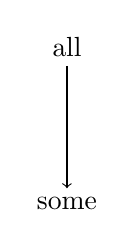
\begin{tikzpicture}
		\node[] at(0, 0) (A) {all};
		\node[] at(0, -2) (B) {some};
		\draw[->] (A) -- (B);
	\end{tikzpicture}
	\caption[]{Directed graph induced by $\vDash$ on $\lbrace \textit{all}, \textit{some}.\rbrace$}\label{fig7:entailment-graph-scalar1}
\end{figure}


The fact that \textit{all} and \textit{some} have same granularity has direct consequences regarding the Qtrees evoked by the simplex sentences involving such quantifiers. Indeed, the layers of ``\textit{wh}'' Qtrees correspond to the Hamblin partition of the CS induced by same-granularity alternatives.

In the case of sentences involving \textit{some} or \textit{all}, the set of same-granularity alternatives is always the same: it is made of the \textit{some}- and \textit{all}-alternatives to the sentence. The partition induced on the CS by such alternatives, therefore splits the CS into \textit{none}-, \textit{some but not all}-, and \textit{all}-worlds. As a result, ``\textit{wh}'' Qtrees evoked by simplex LFs involving \textit{all} or \textit{some}, will always have their leaves partition the CS into \textit{none}- (abbreviated $\neg\exists$), \textit{some but not all}- (abbreviated $\exists\wedge\neg\forall$), and \textit{all}-worlds (abbreviated $\forall$). If no other scalemate is relevant (our focus here),
%\footnote{Appendix \ref{sec7:ded} will explore the predictions of our framework when scalemates of intermediate strength like \textit{most} are considered. In that case, (\ref{ex7:qtree-simplex-def}\ref{pt7:simplex-qtree-tiered}) becomes relevant, and a general update of the ``recipe'' in (\ref{ex7:qtree-simplex-def}) is in fact needed.}
then no alternative coarser-grained than \textit{some} and/or \textit{all} is available, and the resulting Qtrees do not display intermediate layers, i.e. have depth $1$. This gives rise to the Qtrees for $S_{s}$ = \textit{Jo read some of the books} in Figure \ref{fig7:qtrees-some}, and for $S_{s^+}$ = \textit{Jo read all of the books} in Figure \ref{fig7:qtrees-all}. 

\begin{figure}[H]
	\centering
	\begin{subfigure}[b]{.45\linewidth}
		\centering
		\begin{forest}
			[CS[$\neg\exists$][\fbox{$\exists$}]]
		\end{forest}
		\caption[]{``Polar''.}\label{fig7:qtree-some-polar}
	\end{subfigure}
	\hfill
	\begin{subfigure}[b]{.45\linewidth}
		\centering
		\begin{forest}
			[CS[$\neg\exists$][\fbox{$\exists\wedge\neg\forall$}][\fbox{$\forall$}]]
		\end{forest}
		\caption[]{``\textit{Wh}''.}\label{fig7:qtree-some-wh}
	\end{subfigure}
	\caption[]{Qtrees evoked by $S_{\s}$ = \textit{Jo read some of the books}. }\label{fig7:qtrees-some}
\end{figure}


\begin{figure}[H]
	\centering
	\begin{subfigure}[b]{.45\linewidth}
		\centering
		\begin{forest}
			[CS[$\neg\forall$][\fbox{$\forall$}]]
		\end{forest}
		\caption[]{``Polar''.}\label{fig7:qtree-all-polar}
	\end{subfigure}
	\hfill
	\begin{subfigure}[b]{.45\linewidth}
		\centering
		\begin{forest}
			[CS[$\neg\exists$][$\exists\wedge\neg\forall$][\fbox{$\forall$}]]
		\end{forest}
		\caption[]{``\textit{Wh}''.}\label{fig7:qtree-all-wh}
	\end{subfigure}
	\caption[]{Qtrees evoked by $S_{\splus}$ = \textit{Jo read all of the books}. }\label{fig7:qtrees-all}
\end{figure}

Crucially, the two ``\textit{wh}'' Qtrees in these Figures are structurally identical. This differs from the \textit{Noto} vs. \textit{Italy} case, in which ``\textit{wh}'' Qtrees evoked by \textit{Noto} are finer-grained than (and \textit{a fortiori} structurally different from) ``\textit{wh}'' Qtrees evoked by \textit{Italy}. Further disjoining the Qtrees in Figures \ref{fig7:qtrees-some} and \ref{fig7:qtrees-all}, yields only one well-formed output, shown in Figure \ref{fig7:qtree-shd}, which corresponds to the union of Figures \ref{fig7:qtree-some-wh} and \ref{fig7:qtree-all-wh}, i.e. the two structurally identical ``\textit{wh}'' Qtrees we just talked about. One can  easily verify that other possible unions of Qtrees from Figures \ref{fig7:qtrees-some} and \ref{fig7:qtrees-all}, do not yield proper partitions of the CS at the leaf level.

\begin{figure}[H]
	\centering
	\begin{forest}
		[CS[$\neg\exists$][\fbox{$\exists\wedge\neg\forall$}][\fbox{$\forall$}]]
	\end{forest}
	\caption[]{Qtree for (\ref{ex7:shd-ws}) or (\ref{ex7:shd-sw}), obtained from Tree \ref{fig7:qtrees-some} $\vee$ Tree \ref{fig7:qtrees-all}.}\label{fig7:qtree-shd}
\end{figure}

This Qtree is identical to the Qtree in Figure \ref{fig7:qtrees-some} used to form it. Therefore, the two bare scalar HDs in (\ref{ex7:shd}) are so far predicted to be odd due to a violation of \textsc{Q-Non-Redundancy}. To avoid such a violation in the case of (\ref{ex7:shd-ws}), at least one of the two input Qtrees must be altered in such a way that the union between the altered Qtree and some Qtree evoked by the other disjunct, is well-formed, and not odd (in particular, not \textsc{Q-Redundant}). The key, non \textsc{Q-Redundant} Qtree structure we will be after from now on, takes the form of Figure \ref{fig7:qtree-desideratum}. Note that this Qtree can be obtained by ``plugging'' a Qtree for \textit{some}, into the \textit{not all} leaf of a ``polar'' Qtree for \textit{all}.

\begin{figure}[H]
	\centering
	\begin{tabular}{ccccc}
		\begin{forest}
			[CS[$\neg\forall$[$\neg\exists$][\fbox{$\exists\wedge\neg\forall$}]][\fbox{$\forall$}]]
		\end{forest}
		&
		=
		&
		\begin{forest}
			[CS[$\neg\forall$][\fbox{$\forall$}]]
		\end{forest}
		&
		$\cup$
		&
		\begin{forest}
			[{CS$\cap\neg\forall$} [$\neg\exists$][\fbox{$\exists\wedge\neg\forall$}]]
		\end{forest}
	\end{tabular}
	\caption{A reasonable depth-$2$ Qtree for scalar HDs that cannot be \textsc{Q-Redundant}, i.e. a desideratum to predict felicity.}\label{fig7:qtree-desideratum}
\end{figure}

We will see that this desired Qtree, will be derivable in certain cases, in particular in bare and \textit{only}-marked scalar HDs in which \textit{some} occurs in the second disjunct ((\ref{ex7:shd-ws}) and (\ref{ex7:shdo-sw})). This will be demonstrated by assuming that exhaustifiers like \textit{exh} and \textit{only}, affect Qtrees in ways consistent with reasonable assumptions about their core semantics, but also constrained by external, and general, pragmatic constraints. The next Section reviews and motivates these core semantic assumptions and pragmatic constraints.

\subsection{Basic assumptions about (c)overt exhaustifiers}\label{sec7:exh-presupp-assumptions}

So far, we have entertained the rough assumption that \textit{exh} and \textit{only} lead to the same kind of inference. For instance, \textit{exh some} and \textit{only some}, both seem to imply \textit{not all}. And we have so far implicitly assumed that this kind of inference was active at the assertive level with both \textit{exh} and \textit{only}.

There is however a lot of evidence that the inferences triggered by \textit{exh} and \textit{only} are not drawn at the same level. Starting with \textit{only}, a prominent view is that \textit{only p} presupposes its prejacent and asserts the negation of non-weaker alternatives \parencite{Horn1972,Horn1996,Rooth1985,Rooth1992,Roberts2006,Alxatib2013}.\footnote{For different or more elaborate approaches, see e.g. \textcite{Atlas1993,Horn2002,Roberts2011,Crnic2024}.} This is supported by the \textit{Hey, wait a minute!} test, which highlights backgrounded material in a conversation \parencite{vonFintel2004,Shannon1976}. (\ref{ex7:only-hwam}) exemplifies this in the case of \textit{only some}. 

\begin{exe}
	\ex {Al: Jo read only some of the books.\\
		Ed: Hey wait a minute! I did not know Jo read some!
	}\label{ex7:only-hwam}
\end{exe}

The presuppositional status of \textit{only}'s prejacent is also supported by the observation that, if \textit{only p} gets embedded under negation, the inference that $p$ holds is still there. This is exemplified by (\ref{ex7:only-neg}) in the case of \textit{only some}.

\begin{exe}
	\ex {It's not true Jo read only some of the books.\\
		$\leadsto$ Jo read some of the books.
	}\label{ex7:only-neg}
\end{exe}


The second claim that we build on here, is that the covert counterpart of \textit{only} is also its mirror image, in terms of how it divides the work between presupposition and assertion \parencite{Bassi2021,DelPinal2024}. This operator, called \textit{pex} for \textit{presuppositional exh}, is therefore assumed to assert its prejacent and to presuppose the negation of Innocently Excludable alternatives to the prejacent. Testing the validity of this claim in unembedded contexts using the \textit{Hey, wait a minute!} test, or negation, is challenging, because \textit{exh}/\textit{pex} is \textit{a priori} optional in such environments. The presuppositional approach to \textit{exh} is however motivated by inferences arising from exhaustification embedded in specific environments (\textit{some} under \textit{some}, among others) -- that we will not cover here. Additionally, the fact that the inference resulting from \textit{pex p} does not ``feel'' presuppositional, has been attributed to the process of \textit{accommodation}, which amounts to the following. When a presupposition is not met in a given CS, it can be adopted ``on the fly'' and as such shrinks the Context Set just like a regular assertion would do \parencite{Stalnaker1974,Stalnaker2002,vonFintel2008}. A definition of presupposition accommodation is given in (\ref{ex7:presupp-accommodation}). We will soon elaborate on this definition to define the action of \textit{pex p} and \textit{only p} have on Qtrees.

\begin{exe}
	\ex {\textbf{\textsc{Presupposition Accommodation}}. Let $\mathcal{C}$ be a conversation and $CS(\mathcal{C})$ its associated Context Set. Let $A_p$ be an assertion presupposing $p$. If $p$ is not entailed by $CS(\mathcal{C})$, i.e. $CS(\mathcal{C}) \cap \neg p \neq \emptyset$, then $p$ may be accommodated on $CS(\mathcal{C})$, by producing a new Context Set $C' = CS(\mathcal{C})\cap p$, which can be subsequently updated with $A$.}\label{ex7:presupp-accommodation}
\end{exe}
	
Given this, the entries we assume for \textit{only} and \textit{pex} are given in (\ref{ex7:only-entry}) and (\ref{ex7:pex-entry}) respectively. In these entries, presuppositions are underlined.

\begin{exe}
	\ex \label{ex7:pex-only-entries}
	\begin{xlist}
		\ex {$\llbracket$ only $\rrbracket$ = $\lambda p. \ \lambda Q. \ \underline{p}. \ \bigwedge_{p' \in IE(Q, p)} \neg p'$ }\label{ex7:only-entry}
		\ex {$\llbracket$ pex $\rrbracket$ = $\lambda p. \ \lambda Q. \ \underline{\bigwedge_{p' \in IE(Q, p)} \neg p'}. \ p$ }\label{ex7:pex-entry}
	\end{xlist}
\end{exe}

In the specific case of $\langle$\textit{some}, \textit{all}$\rangle$ scalemates, if the prejacent $p$ corresponds to \textit{some}, and its set of relevant alternatives $Q$ corresponds to $\lbrace \textit{some}, \textit{all} \rbrace$, then $\bigwedge_{p' \in IE(Q, p)} \neg p'$ simply corresponds to \textit{not all}. Applying \textit{only} and \textit{pex} to \textit{Jo read some of the books} then gives rise to the meanings in (\ref{ex7:only-some-entry}) and (\ref{ex7:pex-some-entry}) respectively. In brief, the two entries given in (\ref{ex7:pex-only-entries}) predict that \textit{only some} presupposes \textit{some} and asserts \textit{not all}, while \textit{pex some} presupposes \textit{not all} and asserts \textit{some}.
\begin{exe}
	\ex \label{ex7:pex-only-some}
	\begin{xlist}
		\ex {$\llbracket$ Jo read only some of the books $\rrbracket$ = \underline{$\lambda w. \ $ Jo read some of the books in $w$}.\\
			\phantom{$\llbracket$ Jo read only some of the books $\rrbracket$ =} $\lambda w. \ $ Jo did not read all of the booksin $w$}\label{ex7:only-some-entry}
		\ex {$\llbracket$ Jo read pex some of the books $\rrbracket$ = \underline{$\lambda w. \ $ Jo did not read all of the books in $w$}.\\
			\phantom{$\llbracket$ Jo read pex some of the books $\rrbracket$ =} $\lambda w. \ $ Jo red some of the books in $w$}\label{ex7:pex-some-entry}
	\end{xlist}
\end{exe}

If the presupposition of (\ref{ex7:only-some-entry}) were not met, accommodation would lead to intersect the CS with the proposition that \textit{Jo read some of the books}. If the presupposition of (\ref{ex7:pex-some-entry}) were not met, accommodation would lead to intersect the CS with the proposition that \textit{Jo did not read all of the books}.\\


Before moving on, let us review one argument in favor of that view of overt and covert exhaustifiers. This will also be the occasion to introduce a key constraint we will exploit in the following Sections. \textcite{Heim2015} first noticed in lecture notes that overt questions cannot be fully addressed by accommodated presuppositions. This was further formalized by \textcite{Doron2024} in the form of a Post-Accommodation Informativity (henceforth \textbf{PAI}) Constraint. This constraint, given in (\ref{ex7:post-acc-info}), states that, when considering a question-answer pair whereby the answer presupposes $p$, the shrinkage of the partitioned Context Set (corresponding to the question) produced by the accommodation of $p$, should not completely trivialize the question, i.e. should leave space for the assertive component of the answer to rule out at least one remaining cell.

\begin{exe}
	\ex {\textbf{\textsc{Post-Accommodation Informativity (PAI).} } Let $A_p$ be an assertion carrying a presupposition $p$, and let $Q$ be the QuD. Then, $A_p$ must remain informative w.r.t. $Q$ \textit{after} $p$ gets accommodated. Informativity is understood as \textsc{\citeauthor{Roberts2012}'s Relevance}, i.e. as the capacity to rule out at least one cell.}\label{ex7:post-acc-info}
\end{exe}

Let us now briefly review how this applies to question-answer pairs involving scalar expressions. First, assume a QuD about \textit{all}, vs. \textit{not all}, as in (\ref{ex7:q-all-not-all}). It is reasonable to assume that this overt QuD partitions the CS into \textit{all}- and \textit{not all}-worlds. Answering this QuD with \textit{all}, \textit{not all}, or \textit{only some}, is fine; while answering with \textit{some}, or its focused counterpart \textit{SOME}, is degraded. Let us unpack these observations.

\begin{exe}
	\ex {Did Jo do all of the readings, or not all of them?}\label{ex7:q-all-not-all}
	\begin{xlist}
		\ex[] {Jo did all of them.}
		\ex[] {Jo did not do all of them. \hfill (P: Jo did some of them.)}
		\ex[\#] {Jo did some of them. \hfill (P: Jo did not do all of them.)}
		\ex[\#] {Jo did SOME of them. \hfill P: Jo did not do all of them.}
		\ex[] {Jo did only some of them. \hfill P: Jo did some of them.}
	\end{xlist}
\end{exe}

The felicity of the \textit{all}-answer in (\ref{ex7:q-all-not-all}) is unsurprising given PAI and more generally what we know about \textsc{Relevance}: bare \textit{all} does not presuppose anything, and additionally rules out the \textit{not all} cell of the QuD, so is \textsc{\citeauthor{Roberts2012}-Relevant} post-accommodation -- satisfying PAI.

The felicity of the \textit{not all}-answer is also quite easy to explain: the reverse \textit{some} implicature associated with \textit{not all} may not be drawn at all, and since \textit{not all} rules out the \textit{all} cell of the QuD, it is \textsc{\citeauthor{Roberts2012}-Relevant}.

Now turning to the case of \textit{SOME}: focus was previously assumed to activate alternatives and in turn force implicatures \parencite{Rooth1992,Chierchia2011}. Under the \textit{pex}-view, such implicatures are presuppositional, which means that a focused \textit{SOME}-answer is expected to force the accommodation of \textit{not all} \parencite{Bassi2021}. Accommodating this presupposition on the \textit{all} vs. \textit{not all} QuD, reduces this QuD to only one cell: the \textit{all}-cell. The assertion carried by \textit{SOME} (\textit{some}) is then unable to rule out any remaining cell, and, as per PAI, the \textit{SOME}-answer is correctly predicted to be degraded. 

This kind of reasoning extends to the unfocused \textit{some}-answer in the following way: either \textit{some} does not carry any presupposition, in which case \textit{some} is simply \textsc{\citeauthor{Roberts2012}-Irrelevant}, due to being compatible with both the \textit{all} and the \textit{not all} cells of the QuD. Or, \textit{some} carries a \textit{not all} presupposition, and violates PAI just like \textit{SOME} does. 

Lastly, the felicity of the \textit{only some}-answer, is captured by PAI as well. This is because \textit{only some} carries \textit{some} as presupposition. Accommodating this presupposition on the \textit{all} vs. \textit{not all} QuD, produces a ``shrunk'' \textit{all} vs. \textit{some but not all} QuD. And since the assertion conveyed by \textit{only some}, namely \textit{not all}, rules out the \textit{all}-cell of this updated QuD, \textit{only some} is \textsc{\citeauthor{Roberts2012}-Relevant} post-accommodation -- satisfying PAI.\\


Secondly, the same line of reasoning mainly applies, supposing the overt QuD is about \textit{some} vs. \textit{none}, as in (\ref{ex7:q-some-none}). It is reasonable to assume that this overt QuD partitions the CS into \textit{some}- and \textit{none}-worlds. Answering this QuD with \textit{all}, \textit{not all}, \textit{SOME} or \textit{only some}, is degraded or at least off; while answering with \textit{some}, is fine. Let us unpack these observations.

\begin{exe}
	\ex {Did Jo do some of the readings, or none of them?}\label{ex7:q-some-none}
	\begin{xlist}
		\ex[??] {Jo did all of them.}
		\ex[??] {Jo did not do all of them. \hfill (P: Jo did some of them.)}
		\ex[] {Jo did some of them. \hfill (P: Jo did not do all of them.)}
		\ex[\#] {Jo did SOME of them. \hfill P: Jo did not do all of them.}
		\ex[\#] {Jo did only some of them. \hfill P: Jo did some of them.}
	\end{xlist}
\end{exe}

Starting with the \textit{all}-answer, oddness does not come from a violation of PAI, but rather from overinformativity: on top of ruling out the \textit{none}-cell of the QuD, \textit{all} strictly entails the \textit{some}-cell. In other words, the \textit{all}-answer, though \textsc{\citeauthor{Roberts2012}-Relevant}, is not \textsc{\citeauthor*{Lewis1988}-Relevant}.\\

The \textit{only some}-answer on the other hand, happens to violate PAI in the following way: \textit{only some} is expected to accommodate \textit{some}. Accommodating this presupposition on the \textit{some} vs. \textit{none} QuD, reduces this QuD to only one cell: the \textit{some}-cell. The assertion carried by \textit{only some}, namely \textit{not all}, is then unable to rule out any remaining cell, and, as per PAI, the \textit{only some}-answer is correctly predicted to be degraded.

This extends to the \textit{not all}-answer: if \textit{not all} does not carry any presupposition, it is simply \textsc{\citeauthor{Roberts2012}-Irrelevant}, due to being compatible with both the \textit{some} and the \textit{none} cells of the QuD. If \textit{not all} carries a \textit{some} presupposition (traditionally called ``reverse/indirect'' implicature), then, \textit{not all} violates PAI just like \textit{only some} does.

Lastly, the felicity of the \textit{some}-answer in (\ref{ex7:q-some-none}) is relatively unsurprising: bare \textit{some} may not presuppose anything, in which case it rules out the \textit{none} cell of the QuD, so is \textsc{\citeauthor{Roberts2012}-Relevant} post-accommodation. And even if \textit{some} \textit{did} presuppose \textit{not all}, accommodating this presupposition on the \textit{some} vs. \textit{none} QuD, would produce a ``shrunk'' \textit{some but not all} vs. \textit{none} QuD. And since the assertion carried by \textit{some}, correctly rules out the \textit{none}-cell of this updated QuD; \textit{some} would in any case be \textsc{\citeauthor{Roberts2012}-Relevant} post-accommodation, satisfying PAI.\footnote{Why focused \textit{SOME} is degraded in (\ref{ex7:q-some-none}) remains a bit unclear.}\\

We have just seen that PAI, combined with the assumption that overt and covert exhaustifiers are mirror images when it comes to their presuppositions and assertions, explains why a \textit{whether all}-question is incompatible with a \textit{some}-answer and compatible with an \textit{only some}-answer -- see (\ref{ex7:q-all-not-all}). This pattern should look familiar: it appears reminiscent of what happens in bare and \textit{only}-marked scalar HDs in which \textit{all} is the first disjunct, and \textit{(only) some} is the second disjunct. Assuming the first disjunct evokes an ``\textit{all}''-question and the second disjunct provides an ``\textit{(only) some}''-answer, PAI has the potential to explain the asymmetry in bare scalar HDs, and the rescuing effect of \textit{only}.

To clarify this intuition, we proceed to derive the effect of \textit{exh} and \textit{only} on Qtrees, building their assumed semantic entries, and furthermore adapt PAI to the incremental Qtree framework.


\subsection{Effect of presuppositions on Qtrees}

We now argue that the difference between \textit{pex} and \textit{only} in terms of how they divide presupposition and assertion, has consequences beyond truth and definedness conditions. Namely, we submit that \textit{pex} and \textit{only} differentially interact with Qtrees, in ways consistent with how their presuppositions would be standardly accommodated.

Taking inspiration from the theory of Local Contexts \parencite{Schlenker2009}, we submit that presuppositions interact with Qtrees in systematic ways -- characterized by both \textit{locality} and \textit{incrementality}. Here is a very schematic interpretation of the theory of Local Context we take inspiration from. Very broadly, at each point of the processing of a sentence, some material, that we will call \textbf{current material} is being evaluated against a function of \textbf{past material}. For instance, under an asymmetric view of disjunction, the first disjunct is typically evaluated against no past material; while the second disjunct is typically evaluated against a past material dependent on the first disjunct. This is schematized in (\ref{ex7:disj-incr}), whereby the $|$-notation implies that a constituent (to the left of $|$) is evaluated given extra information (to the right of $|$).

\begin{exe}
	\ex \label{ex7:disj-incr}
	\begin{xlist}
		\ex {\textbf{Current material or} ...}
		\ex {{Past material or} (\textbf{Current material}$|$$f$({Past material}))
		}
	\end{xlist}
\end{exe}

Specifically, whenever the current material triggers a presupposition, this presupposition gets evaluated against a Local Context Set inferred from the past material. In the case of disjunction, the asymmetric processing assumption predicts that the first disjunct is evaluated against the global CS, while the second disjunct is evaluated against a local CS intersected with the negation of the first disjunct.

\begin{exe}
	\ex \label{ex7:disj-incr-lc}
	\begin{xlist}
		\ex {(\textbf{Current material}$|$CS) \textbf{or} ...}
		\ex {{Past material or} (\textbf{Current material}$|$CS$\cap\neg${Past material})
		}
	\end{xlist}
\end{exe}

This explains why a sentence like (\ref{ex:presupp-local}), does not globally presuppose that \textit{Jo is French}, despite the fact that it is presupposed by the second disjunct \textit{Al know that Jo is French}. This presupposition gets locally satisfied at the level of the second disjunct (current material), after the first disjunct (past material) is processed. Indeed, processing the first disjunct creates a Local Context Set that entails the negation of \textit{Jo is not French}, i.e. that \textit{Jo is French}.

\begin{exe}
	\ex {Either Jo is not French, or Al know that Jo is French.}\label{ex:presupp-local}
\end{exe}


We extend this view to Qtrees: when processing a sentence, ``incremental'' Qtrees can be inferred from the past material. These  ``incremental'' Qtrees can be seen as analog to a Local Context Set. This is (very roughly) schematized in (\ref{ex7:disj-incr-qtree}).

\begin{exe}
	\ex \label{ex7:disj-incr-qtree}
	\begin{xlist}
		\ex {(\textbf{Current material}) \textbf{or} ...}
		\ex {{Past material or} (\textbf{Current material}$|$Qtrees({Past material}))
		}
	\end{xlist}
\end{exe}

Here is a more detailed description of the process we propose. First, the felicity of the current material gets evaluated against the possible ``incremental'' Qtrees. We will define this evaluation step as a variant of PAI, which means that it will assign a crucial role to the presupposition -- if any -- carried by the current material. It will also be phrased in a way that will allow us to rule out certain Qtrees evoked by past material. If this evaluation step is successful for at least some Qtrees, then whatever presupposition is carried by the current material can be locally incorporated to the the Qtrees evoked by the current material. We will see that this  ``incorporation'' constitutes a generalization of what accommodation is normally assumed to do; additionally it will be heavily driven by how the incremental Qtree divides up the CS. After the presupposition is incorporated to the current material, the computation of Qtrees can proceed as usual, and is subject to all the constraints we introduced in previous Chapters. This view of the interaction between embedded presupposition and (incremental) Qtrees, is summarized in (\ref{ex7:qtree-presupp-interplay}).

\begin{exe}
	\ex {\textsc{\textbf{General interplay between Qtrees and presuppositions.}} Assume a sentence is incrementally processed, $X$ being the past material (a partial LF) and $Y$ the current material (a full LF). Let us assume that $Y$ involves a presupposition trigger, s.t. $\llbracket Y \rrbracket$ presupposes $p$. Two cases:
	\begin{itemize}
		\item If $X$ is empty, then $Y$ is ``out-of-the-blue'' and $p$ gets accommodated on $Y$'s Qtrees, prior to further Qtree computations.
		\item If $X$ is not empty, then $Y$ and its presupposition $p$ must be evaluated against the incremental Qtrees inferred from $X$. If this evaluation step is successful for a given incremental Qtree $T$, then $T$'s leaves compatible with $p$ are accommodated on $Y$'s Qtrees, prior to further Qtree computations.
	\end{itemize}}\label{ex7:qtree-presupp-interplay}
\end{exe}

The definition in (\ref{ex7:qtree-presupp-interplay}) appeals to three notions that the rest of this Section will clarify: the notion of presupposition accommodation on a Qtree, the notion of incremental Qtrees inferred from a partial LF, and the notion of evaluation against an incremental Qtree. The rest of this Section unpacks these definitions, relating them to standard views on presuppositions and their interaction with questions.

\subsubsection{Accommodation on Qtrees}

In the previous Section, (\ref{ex7:presupp-accommodation}) defined presupposition accommodation as the intersection between a presupposition and the CS. Given this standard definition, and that Qtrees can be seen as parses (or nested partitions) of the CS, accommodating a presupposition on a Qtree, naturally amounts to intersecting the entire Qtree, with the presupposition. This is exactly what tree-node intersection achieves. This is restated in (\ref{ex7:qtree-accommodation}).

\begin{exe}
	\ex {\textbf{\textsc{Presupposition Accommodation on Qtrees}}. Let $p$ be a presupposition and $T$ a Qtree. Accommodating $p$ on $T$ amounts to computing $T\cap p$, where $\cap$ designates the tree-node intersection operation defined in (\ref{ex2:nodewise-inter}).}\label{ex7:qtree-accommodation}
\end{exe}

In brief, (\ref{ex7:qtree-accommodation}) maintains the idea that assertions evoke Qtrees (structure, and verifying nodes), but adds to this that (locally) accommodated presuppositions further intersect Qtrees evoked by assertions. In that sense, presuppositions do not evoke ways to parse the CS, but instead give directions on how to restrict it.\\


Let us now see which Qtrees result from the accommodation of \textit{not all}, and \textit{some}, on Qtrees evoked by \textit{all}. Why we choose to exemplify these precise operations, will be made clear in the next Sections, but at that point let us note that \textit{all} corresponds to the presuppositionless disjunct of scalar HDs, while \textit{not all} and \textit{some} correspond to the presuppositions carried by \textit{pex some} and \textit{only some}, respectively. Qtrees evoked by \textit{all} are repeated in Figure \ref{fig7:qtrees-all-r}.

\begin{figure}[H]
	\centering
	\begin{subfigure}[b]{.45\linewidth}
		\centering
		\begin{forest}
			[CS[$\neg\forall$][\fbox{$\forall$}]]
		\end{forest}
		\caption[]{``Polar''.}\label{fig7:qtree-all-polar-r}
	\end{subfigure}
	\hfill
	\begin{subfigure}[b]{.45\linewidth}
		\centering
		\begin{forest}
			[CS[$\neg\exists$][$\exists\wedge\neg\forall$][\fbox{$\forall$}]]
		\end{forest}
		\caption[]{``\textit{Wh}''.}\label{fig7:qtree-all-wh-r}
	\end{subfigure}
	\caption[]{Qtrees evoked by $S_{\splus}$ = \textit{Jo read all of the books}. }\label{fig7:qtrees-all-r}
\end{figure}

Intersecting these Qtrees with \textit{not all}, leads to the two ``shrunk'' Qtrees in Figure \ref{fig7:qtrees-all-inter-notall}. Intersection with \textit{not all} caused the input Qtree in Figure \ref{fig7:qtree-all-polar-r} to lose a leaf and be reduced to a single root. Intersection with \textit{not all} caused the input Qtree in Figure \ref{fig7:qtree-all-wh-r} to lose a leaf as well.

\begin{figure}[H]
	\centering
	\begin{subfigure}[b]{.45\linewidth}
		\centering
		\begin{forest}
			[{CS$\cap\neg\forall$}]
		\end{forest}
		\caption[]{Tree \ref{fig7:qtree-all-polar-r} $\cap\neg\forall$}\label{fig7:qtree-all-polar-inter-notall}
	\end{subfigure}
	\hfill
	\begin{subfigure}[b]{.45\linewidth}
		\centering
		\begin{forest}
			[{CS$\cap\neg\forall$}[$\neg\exists$][$\exists\wedge\neg\forall$]]
		\end{forest}
		\caption[]{Tree \ref{fig7:qtree-all-wh-r} $\cap\neg\forall$.}\label{fig7:qtree-all-wh-inter-notall}
	\end{subfigure}
	\caption[]{Accommodating \textit{not all} on Qtrees evoked by $S_{\splus}$ = \textit{Jo read all of the books}. }\label{fig7:qtrees-all-inter-notall}
\end{figure}

Intersecting the Qtrees evoked by \textit{all}, with \textit{some}, leads to only one ``shrunk'' Qtree, given in Figure \ref{fig7:qtrees-all-inter-some}. In other words, intersection with \textit{some} collapses the two Qtrees evoked by \textit{all} in Figure \ref{fig7:qtrees-all-r}, into one single output with two leaves.

\begin{figure}[H]
	\centering
		\begin{forest}
			[{CS$\cap\exists$}[$\exists\wedge\neg\forall$][\fbox{$\forall$}]]
		\end{forest}
		\caption[]{Tree \ref{fig7:qtree-all-polar-r} / \ref{fig7:qtree-all-wh-r} $\cap\exists$}\label{fig7:qtree-all-polar-inter-some}
	\caption[]{Accommodating \textit{some} on Qtrees evoked by $S_{\splus}$ = \textit{Jo read all of the books}. }\label{fig7:qtrees-all-inter-some}
\end{figure}

The next Section further motivates these moves, by arguing that the presuppositions of \textit{pex some} (\textit{not all}) or \textit{only some} (\textit{some}) locally drawn in scalar HDs, are constrained by the Qtree evoked by past material (and vice versa).




%
%
%applies to \textit{pex some} and \textit{only some}. We know that \textit{pex some} presupposes \textit{not all} and asserts \textit{some}. So \textit{not all} gets to be locally accommodated on the Qtrees evoked by \textit{some}. This implies that the Qtrees evoked by \textit{some} given in Figure \ref{fig7:qtrees-some}, get intersected with \textit{not all}-worlds. This operation collapses the two possible inputs from Figure \ref{fig7:qtrees-some}, into just one output, given in Figure \ref{fig7:qtree-some-polar-inter-notall}.\footnote{Given that tree-node intersection is constrained by \textsc{Incremental Q-Relevance}, we should in principle verify that the output Qtree in Figure \ref{fig7:qtree-some-inter-notall} can be formed \textit{via} a \textsc{Relevant} derivation as per (\ref{ex6:incremental-q-relevance}). It can be shown that this is the case.} 
%
%\begin{figure}[H]
%	\centering
%	\begin{forest}
%		[CS$\cap\neg\forall$[$\neg\exists$][\fbox{$\exists\wedge\neg\forall$}]]
%	\end{forest}
%	\caption[]{Tree \ref{fig7:qtree-some-wh} $\cap$ \textit{not all}.}\label{fig7:qtree-some-inter-notall}
%\end{figure}
%
%
%
%
%
%(\ref{ex7:qtree-accommodation-2}) is yet still insufficient to predict the felicity of \textit{only}-marked HDs like those in (\ref{ex7:shdo}). Let us see how far we can go with this principle, and what its failure teaches us. We know that \textit{only some} presupposes \textit{some} and asserts \textit{not all}. So \textit{some} gets to be locally accommodated on the Qtrees evoked by \textit{not all}. This implies that the Qtrees evoked by \textit{not all}, given in Figure \ref{fig7:qtrees-not-all}, get intersected with \textit{some}-worlds.
%
%\begin{figure}[H]
%	\centering
%	\begin{subfigure}[b]{.45\linewidth}
%		\centering
%		\begin{forest}
%			[CS[\fbox{$\neg\forall$}][{$\forall$}]]
%		\end{forest}
%		\caption[]{``Polar''.}\label{fig7:qtree-not-all-polar}
%	\end{subfigure}
%	\hfill
%	\begin{subfigure}[b]{.45\linewidth}
%		\centering
%		\begin{forest}
%			[CS[\fbox{$\neg\exists$}][\fbox{$\exists\wedge\neg\forall$}][{$\forall$}]]
%		\end{forest}
%		\caption[]{``\textit{Wh}''.}\label{fig7:qtree-not-all-wh}
%	\end{subfigure}
%	\caption[]{Qtrees evoked by $\neg S_{\splus}$ = \textit{Jo did not read all of the books}. }\label{fig7:qtrees-not-all}
%\end{figure}
%
%This operation collapses the two possible inputs from Figure \ref{fig7:qtrees-not-all}, into just one output, given in Figure \ref{fig7:qtree-not-all-inter-some}. Given that tree-node intersection is constrained by \textsc{Incremental Q-Relevance}, we must again verify that the output Qtree in Figure \ref{fig7:qtree-not-all-inter-some} can be formed \textit{via} a \textsc{Relevant} derivation as per \ref{ex6:incremental-q-relevance}. Considering the ``\textit{wh}'' Qtree for \textit{not all} (in Figure \ref{fig7:qtree-not-all-wh}) as input, the tree-node intersection with \textit{some} performed to produce Figure \ref{fig7:qtree-not-all-inter-some} is indeed \textsc{Relevant}, because it rules out one leaf of the original Qtree (the \textit{none}-leaf), and retains at least one leaf (in fact, two leaves, the \textit{all} and the \textit{some but not all} leaves). Therefore, there is a way to generate the Qtree in Figure \ref{fig7:qtree-not-all-inter-some} that does not violate \textsc{Incremental Q-Relevance}, and this Qtree is well-formed. Note that this reasoning is completely symmetric to the one we conducted in the case of \textit{pex some}.
%
%\begin{figure}[H]
%	\centering
%	\begin{forest}
%		[CS$\cap \exists$[\fbox{$\exists\wedge\neg\forall$}][{$\forall$}]]
%	\end{forest}
%	\caption[]{Tree \ref{fig7:qtree-not-all-polar} / \ref{fig7:qtree-not-all-wh} $\cap$ \textit{some}.}\label{fig7:qtree-not-all-inter-some}
%\end{figure}
%
%The Qtree in Figure \ref{fig7:qtree-not-all-inter-some} can then get disjoined with Qtrees evoked by the stronger disjunct, namely \textit{all}, but this is where a problem arises: disjoinining the the post-accommodation Qtree in Figure \ref{fig7:qtree-not-all-inter-some}, with a Qtree for \textit{all}, never gives rise to a well-formed output, essentially because the root of the Qtree in Figure \ref{fig7:qtree-not-all-inter-some}, denotes a set of \textit{some}-worlds, and this root strictly overlaps with the nodes of the Qtrees evoked by \textit{all}.
%
%\begin{figure}[H]
%	\centering
%	\begin{subfigure}[b]{.45\linewidth}
%		\centering
%		\begin{tikzpicture}
%			\node[] at(0, 0) (some) {$\exists$};
%			\node[] at(1, 0) (cs) {CS};
%			\node[] at(-.5, -1) (sbna) {$\exists\wedge\neg\forall$};
%			\node[] at(.5, -1) (all) {$\forall$};
%			\node[] at(1.5, -1) (notall) {$\neg\forall$};
%			\draw[-] (some) -- (sbna);
%			\draw[-] (some) -- (all);
%			\draw[-] (cs) -- (all);
%			\draw[-] (cs) -- (notall);
%		\end{tikzpicture}
%		\caption[]{Tree \ref{fig7:qtree-all-polar} $\vee$ Tree \ref{fig7:qtree-not-all-inter-some}.}
%	\end{subfigure}
%	\hfill
%	\begin{subfigure}[b]{.45\linewidth}
%		\centering
%		\begin{tikzpicture}
%			\node[] at(0, 0) (some) {$\exists$};
%			\node[] at(1, 0) (cs) {CS};
%			\node[] at(.5, -1) (all) {$\forall$};
%			\node[] at(-.5, -1) (sbna) {$\exists\wedge\neg\forall$};
%			\node[] at(1.5, -1) (none) {$\neg\exists$};
%			\draw[-] (some) -- (sbna);
%			\draw[-] (some) -- (all);
%			\draw[-] (cs) -- (sbna);
%			\draw[-] (cs) -- (none);
%			\draw[-] (cs) -- (all);
%		\end{tikzpicture}
%		\caption[]{Tree \ref{fig7:qtree-all-wh} $\vee$ Tree \ref{fig7:qtree-not-all-inter-some}.}
%	\end{subfigure}
%	\caption[]{Ill-formed Qtrees so far derived for the felicitous \textit{only}-marked HDs in (\ref{ex7:shdo}).}\label{fig7:qtree-shdo}
%\end{figure}

\subsubsection{Incremental Qtrees}

The general definition of the interplay between Qtrees and presuppositions in (\ref{ex7:qtree-presupp-interplay}), stated that current material (including its presuppositions), had to be ``evaluated'' against ``incremental'' Qtrees inferred from past material. Incremental Qtrees inferred from a partial LF, can be understood as Qtrees with underspecified nodes, and whose specified structure can be inferred from past material along with the compositional rules of Qtree derivation defined in Chapter \ref{chap:accommodating-quds}. We will not provide a completely general, inductive definition of such incremental Qtrees, and will instead focus on cases in which the past material is the first disjunct of a disjunction.

It turns out that computing the Qtrees evoked by the first disjunct of a disjunction already provides a lot of information about what the Qtree evoked by the entire disjunction should look like. This is essentially because computing the Qtree of a disjunction amounts to computing all the unions of the Qtrees evoked by the disjuncts. This guarantees that a disjunctive Qtree constitues a refinement ($\simeq$ superset) of the two Qtrees used to form it. So, if the first disjunct of a disjunction evokes a Qtree $T$, one can be sure that the entire disjunctive Qtree will be some refinement of $T$. But there is uncertainty about which leaves of $T$, if any, will be further subdivided. Therefore, in a disjunction, the incremental Qtree computed after processing the first disjunct, is an \textit{arbitrary} refinement of some Qtree evoked by the first disjunct.

Given this, incremental Qtrees  derived after processing \textit{all} as first disjunct, are given in Figure \ref{fig7:sqtrees-all}. In this Figure, the triangles labeled with a question-mark signal underspecification: the root of these triangles may, or may not be further subdivided into more nodes, depending on what the second disjunct will turn out to be. We will assume that \textit{all} and \textit{none} leaves are already maximally informative, and cannot be further partitioned without completely shifting the QuD -- that is why such leaves do not feature ``triangles''. 

%Likewise, incremental Qtrees  derived after processing \textit{some} as first disjunct, are given in Figure \ref{fig7:sqtrees-some}.
\begin{figure}[H]
	\centering
	\begin{subfigure}[b]{.45\linewidth}
		\centering
		\begin{forest}
			[CS[$\neg\forall$[?,roof]][\fbox{$\forall$}]]
		\end{forest}
		\caption[]{``Polar''.}\label{fig7:sqtree-all-polar}
	\end{subfigure}
	\hfill
	\begin{subfigure}[b]{.45\linewidth}
		\centering
		\begin{forest}
			[CS[$\neg\exists$][$\exists\wedge\neg\forall$[?,roof]][\fbox{$\forall$}]]
		\end{forest}
		\caption[]{``\textit{Wh}''.}\label{fig7:sqtree-all-wh}
	\end{subfigure}
	\caption[]{Incremental Qtrees evoked by $S_{\splus} \vee ...$ = \textit{Jo read all of the books or ...}. }\label{fig7:sqtrees-all}
\end{figure}
%\begin{figure}[H]
%	\centering
%	\begin{subfigure}[b]{.45\linewidth}
%		\centering
%		\begin{forest}
%			[CS[$\neg\exists$][\fbox{$\exists$}[?, roof]]]
%		\end{forest}
%		\caption[]{``Polar''.}\label{fig7:sqtree-some-polar}
%	\end{subfigure}
%	\hfill
%	\begin{subfigure}[b]{.45\linewidth}
%		\centering
%		\begin{forest}
%			[CS[$\neg\exists$][\fbox{$\exists\wedge\neg\forall$}[?,roof]][\fbox{$\forall$}]]
%		\end{forest}
%		\caption[]{``\textit{Wh}''.}\label{fig7:sqtree-some-wh}
%	\end{subfigure}
%	\caption[]{Incremental Qtrees evoked by $S_{\s} \vee ...$ = \textit{Jo read some of the books or ...}. }\label{fig7:sqtrees-some}
%\end{figure}

It now becomes possible to combine presupposition accommodation, as defined in (\ref{ex7:qtree-accommodation}), with \textit{incremental} Qtrees. In particular, it is possible to accommodate \textit{not all} and \textit{some}, on incremental Qtrees inferred from \textit{all or...}. This is done in Figures \ref{fig7:sqtrees-all-inter-notall} and \ref{fig7:sqtrees-all-inter-some} respectively. Note that these Figures are the same as Figures \ref{fig7:qtrees-all-inter-notall} and \ref{fig7:qtrees-all-inter-some}, \textit{modulo} the underspecification ``triangles''.

\begin{figure}[H]
	\centering
	\begin{subfigure}[b]{.45\linewidth}
		\centering
		\begin{forest}
			[{CS$\cap\neg\forall$}[?,roof]]
		\end{forest}
		\caption[]{Tree \ref{fig7:sqtree-all-polar} $\cap\neg\forall$.\\ \textbf{Will be shown to be IPAI-violating}.}\label{fig7:sqtree-all-polar-inter-notall}
	\end{subfigure}
	\hfill
	\begin{subfigure}[b]{.45\linewidth}
		\centering
		\begin{forest}
			[{CS$\cap\neg\forall$}[$\neg\exists$][$\exists\wedge\neg\forall$[?, roof]]]
		\end{forest}
		\caption[]{Tree \ref{fig7:sqtree-all-wh} $\cap\neg\forall$.\\ \textbf{Will be shown to be IPAI-compliant}.}\label{fig7:sqtree-all-wh-inter-notall}
	\end{subfigure}
	\caption[]{Accommodating \textit{not all} on incremental Qtrees evoked by $S_{\splus} \vee ...$ = \textit{Jo read all of the books or ...}. }\label{fig7:sqtrees-all-inter-notall}
\end{figure}

\begin{figure}[H]
	\centering
	\begin{forest}
		[{CS$\cap\exists$}[$\exists\wedge\neg\forall$[?,roof]][\fbox{$\forall$}]]
	\end{forest}
	\caption[]{(Tree \ref{fig7:sqtree-all-polar} / \ref{fig7:sqtree-all-wh}) $\cap\exists$. \textbf{Will be shown to be IPAI-compliant}.}\label{fig7:sqtree-all-polar-inter-some}
	\caption[]{Accommodating \textit{some} on incremental Qtrees evoked by $S_{\splus} \vee ...$ = \textit{Jo read all of the books or ...}. }\label{fig7:sqtrees-all-inter-some}
\end{figure}

We will now see how these Qtrees are in fact constrained by the assertions of \textit{pex some} and \textit{only some}, \textit{via} an adaptation of PAI, dubbed \textbf{Incremental PAI}. This constraint will eventually contribute to explaining the difference between bare scalar HDs and \textit{only}-marked HDs.

\subsubsection{Presupposition evaluation against incremental Qtrees}

We now define the concept of evaluation against an incremental Qtree. In Section \ref{sec7:exh-presupp-assumptions}, we  already mentioned that a presupposition carried by the answer to an overt QuD may be accommodated against the partitioned Context Set produced by that QuD. We additionally introduced an independently motivated constraint on this kind of accommodation, in the form of PAI, in (\ref{ex7:post-acc-info}). Roughly, PAI says that accommodation should not trivialize an overt QuD, i.e. allow the assertion conveyed by the answer to rule out a cell in the ``shrunk'', post-accommodation QuD.\\

We now adapt this principle to incremental, implicit QuDs. This gives rise to the ``incremental'' variant of PAI (henceforth \textbf{IPAI}) given in (\ref{ex7:incr-post-acc-info}). This constraint states that, if the presupposition carried by current material trivializes an incremental Qtree inferred from past material, then, this Qtree should no longer be considered for further computations. A Qtree is trivialized by accommodation, if the assertion conveyed by the current material cannot rule out any leaf of that Qtree after accommodation.

\begin{exe}
	\ex {\textbf{\textsc{Incremental Post-Accommodation Informativity (IPAI).} } Let $Y$ be the current material (a full LF) under evaluation. If there is no past material, then IPAI is trivially satisfied. If some past material $X$ is available, let $T$ be an incremental Qtree inferred from $X$. Let us assume that $Y$ involves a presupposition trigger, s.t. $\llbracket Y \rrbracket$ presupposes $p$. Evaluating $Y$ against $T$, amounts to:
		\begin{enumerate}[(i)]
			\item\label{pt7:accommodation} Intersecting $T$ and $p$ \textit{via} tree-node intersection, forming $T\cap p$.\footnote{Note that this imposes that $p$ be in a certain sense \textsc{Relevant} to $T$, as per the \textsc{Incremental Q-Relevance} principle proposed in Chapter \ref{chap:hurford-sentences}.}
			\item\label{pt7:informativity} Checking if at least one leaf of $T \cap p$, is incompatible with (i.e. ruled out by) $Y$'s assertion. \item If the previous test, fails, then $T$ should not be considered for further Qtree computations.
		\end{enumerate}
	If $Y$ does not involve a presupposition trigger, then evaluating $Y$ against $T$, simply amounts to checking if at least one leaf of $T$, is incompatible with (i.e. ruled out by) $Y$'s assertion. If this fails, then $T$ should not be considered for further Qtree computations.\footnote{The same would follow from (\ref{pt7:accommodation}) and (\ref{pt7:informativity})if presuppositionless LFs were taken to carry a contextual tautology as presupposition.}
	}\label{ex7:incr-post-acc-info}
\end{exe}

One important thing to note is that IPAI, unlike PAI, does not deem the current material infelicitous if its presupposition trivializes an incremental Qtree. This partly comes from the fact that there may be multiple possible incremental Qtrees against which the current material can be evaluated. Put differently, IPAI is a constraint on \textit{pairs} formed by incremental Qtrees, and current material; if it is violated on a given pair, IPAI will deem the \textit{Qtree} deviant, and not the current material \textit{per se}. However, we will see that this more subtle move (which is reminiscent of the move we made when we defined \textsc{Q-Non-Redundancy} in Chapter \ref{chap:redundancy}), can sometimes result in global infelicity, if it deems deviant Qtrees that are critical to a felicitous derivation.\\

 
Let us now see how (\ref{ex7:incr-post-acc-info}) applies to bare and \textit{only}-marked scalar HDs. We start with the more complex and interesting cases, in which the presupposition trigger \textit{pex}/\textit{only} occurs in the second disjunct, i.e. (\ref{ex7:shd-sw}) and (\ref{ex7:shdo-sw}), repeated below. Note that \textit{pex} can be assumed to be \textit{needed} in (\ref{ex7:shd-sw}) because we have already seen that this sentence is \textsc{Q-Redundant} without \textit{pex}.

\begin{exe}
	\exr{ex7:shd-sw}[??] {Jo read all or some of the books. \hfill \splus{} $\vee$ \s}
	\exr{ex7:shdo-sw}[] {Jo read all or only some of the books. \hfill $\splus\vee O(\s)$}
\end{exe}

A lot of preliminary work has been done to check IPAI on these structures. Let us first consider (\ref{ex7:shd-sw}). In this sentence, the second disjunct, \textit{pex some}, presupposes \textit{not all} and asserts \textit{some}. To check IPAI, we must evaluate if accommodating \textit{not all} on the incremental Qtrees inferred from \textit{all or ...} (first disjunct), trivializes these Qtrees. We have already computed the intersection between incremental Qtrees for \textit{all or...} and \textit{not all}, in Figure \ref{fig7:sqtrees-all-inter-notall}. What remains to be done, is to check if the assertion of \textit{pex some}, namely \textit{some}, rules out a leaf in such Qtrees. This is not the case in Qtree \ref{fig7:sqtree-all-polar-inter-notall}, simply because the leaves of this Qtree are underspecified, so it is impossible to know if a leaf is ruled out or not. This is the case in Qtree \ref{fig7:sqtree-all-wh-inter-notall}: \textit{some} definitely rules out the \textit{none} leaf. Therefore, the only IPAI-compliant incremental Qtree in the case of (\ref{ex7:shd-sw}), is the one inferred from the  first disjunct's ``\textit{wh}'' Qtree. We will later see that, even if this Qtree satisfies IPAI, disjoining it with a Qtree evoked by the second disjunct, incurs a violation of \textsc{Q-Non-Redundancy}.

We now turn to (\ref{ex7:shdo-sw}). In this sentence, the second disjunct, \textit{only some}, presupposes \textit{some} and asserts \textit{not all}. To check IPAI, we must evaluate if accommodating \textit{some} on the incremental Qtrees inferred from \textit{all or ...} (first disjunct), trivializes these Qtrees. We have already computed the intersection between incremental Qtrees for \textit{all or...} and \textit{some}, in Figure \ref{fig7:sqtrees-all-inter-some}. What remains to be done, is to check if the assertion of \textit{only some}, namely \textit{not all}, rules out a leaf in this Qtrees. This is the case: \textit{not all} definitely rules out the \textit{all} leaf. Therefore, the Qtree in Figure \ref{fig7:sqtrees-all-inter-some}, inferred from the first disjunct's ``\textit{wh}'' Qtree, is IPAI-compliant in the case of (\ref{ex7:shdo-sw}). We will later see that, on top of satisfying IPAI, this Qtree does \textit{not} incur a violation of \textsc{Q-Non-Redundancy} when disjoined with a Qtree evoked by the second disjunct. This will effectively predict the felicity of  (\ref{ex7:shdo-sw}).\\

We now briefly cover scalar HDs in which the presupposition trigger \textit{pex}/\textit{only} occurs in the first disjunct, i.e. (\ref{ex7:shd-ws}) and (\ref{ex7:shdo-ws}), repeated below. Again, \textit{pex} can be assumed to be \textit{needed} in (\ref{ex7:shd-ws}), to rescue this structure from \textsc{Q-Non-Redundancy}.

\begin{exe}
	\exr{ex7:shd-ws}[\#] {Jo read some or all of the books. \hfill $\s\vee\splus$}
	\exr{ex7:shdo-ws}[] {Jo read only some or all of the books. \hfill $O(\s)\vee\splus$}
\end{exe}

In these sentences, the presuppositional disjunct \textit{pex some} or \textit{only some}, is ``out-of-the-blue'' and so is not targeted by IPAI -- see (\ref{ex7:incr-post-acc-info}). According to the general definition in (\ref{ex7:qtree-presupp-interplay}), the presupposition of the first disjunct is directly accommodated on this this disjunct's Qtrees. Starting with (\ref{ex7:shd-ws}), once the first disjunct is processed, \textit{not all} is accommodated on Qtrees evoked by \textit{some}. This is done in Figure \ref{fig7:qtree-some-inter-notall}. The second disjunct, \textit{all}, can then be evaluated against the incrementalized version of this Qtree, in Figure \ref{fig7:sqtree-some-inter-notall}. Because \textit{all} is presupositionless, it is enough to check that \textit{all} rules out a leaf in Qtree \ref{fig7:sqtree-some-inter-notall}. This is the case: \textit{all} is definitely incompatible with \textit{some but not all}, and any leaf this node might have. In sum, IPAI does not rule out any Qtree in (\ref{ex7:shd-ws}).

\begin{figure}[H]
	\centering
	\begin{subfigure}[b]{.45\linewidth}
		\centering
		\begin{forest}
			[CS$\cap\neg\forall$[$\neg\exists$][\fbox{$\exists\wedge\neg\forall$}]]
		\end{forest}
		\caption[]{Accommodating \textit{not all} on Qtrees evoked by $S_{\s}$ = \textit{Jo read some of the books}.}\label{fig7:qtree-some-inter-notall}
	\end{subfigure}
	\hfill
	\begin{subfigure}[b]{.45\linewidth}
		\centering
		\begin{forest}
			[CS$\cap\neg\forall$[$\neg\exists$][\fbox{$\exists\wedge\neg\forall$}[?,roof]]]
		\end{forest}
		\caption[]{Incremental Qtree evoked by $pex (S_{\s}) \vee ...$ = \textit{Jo read pex some of the books or ...}. \textbf{IPAI-compliant}. }\label{fig7:sqtree-some-inter-notall}
	\end{subfigure}
\end{figure}

Now turning to (\ref{ex7:shdo-ws}), once the first disjunct is processed, \textit{some} is  accommodated on Qtrees evoked by \textit{not all}. This is done in Figure \ref{fig7:qtree-notall-inter-some}. The second disjunct, \textit{all}, can then be evaluated against the incrementalized version of this Qtree, in Figure \ref{fig7:sqtree-notall-inter-some}. It is again enough to check that \textit{all} rules out a leaf in Qtree \ref{fig7:sqtree-some-inter-notall}. This is the case: \textit{all} is definitely incompatible with \textit{some but not all}, and any leaf this node might have. In sum, IPAI does not rule out any Qtree in (\ref{ex7:shdo-ws}) either.

\begin{figure}[H]
	\centering
	\begin{subfigure}[b]{.45\linewidth}
		\centering
		\begin{forest}
			[{CS$\cap\exists$}[\fbox{$\exists\wedge\neg\forall$}][{$\forall$}]]
		\end{forest}
		\caption[]{Accommodating \textit{some} on Qtrees evoked by $\neg S_{\splus}$ = \textit{Jo did not read some of the books}. }\label{fig7:qtree-notall-inter-some}
	\end{subfigure}
	\hfill
	\begin{subfigure}[b]{.45\linewidth}
		\centering
		\begin{forest}
			[{CS$\cap\exists$}[\fbox{$\exists\wedge\neg\forall$}[?,roof]][{$\forall$}]]
		\end{forest}
		\caption[]{Incremental Qtree evoked by $only (S_{\s}) \vee ...$ = \textit{Jo read only some of the books or ...}. \textbf{IPAI-compliant}. }\label{fig7:sqtree-notall-inter-some}
	\end{subfigure}
\end{figure}

We have just introduced an incremental version of PAI, IPAI, constraining the interaction between incremental Qtrees (inferred from past material) and current material. We have seen that IPAI crucially rules out the ``polar'' Qtree evoked by the first disjunct in the infelicitous bare scalar HD (\ref{ex7:shd-sw}), because this Qtree gets trivialized by the \textit{not all} presupposition carried by the second disjunct (\textit{pex some}). We will soon see that this Qtree would have been crucial to make this sentence escape \textsc{Q-Non-Redundancy}. In that sense, IPAI will contribute to capturing the asymmetry in scalar HDs.


\subsection{Qtree-driven accommodation}
So far, we have identified accommodation with tree-node intersection, and spelled out how assertions and their potential presuppositions are evaluated against incremental Qtrees -- sometimes resulting in the exclusion of Qtrees (the IPAI-violating ones) from further derivations.

(\ref{ex7:qtree-presupp-interplay}) stated that any incremental Qtree $T$ verifying IPAI, would in turn drive the accommodation of presuppositions on Qtrees evoked by \textit{current material}. Specifically, it was assumed that the leaves of $T$ compatible with the presupposition $p$, may be accommodated on the Qtrees evoked by current material prior to further derivation. We will now see that this Qtree-driven accommodation operation, may eventually enable the desired derivation initially spelled out in Figure \ref{fig7:qtree-desideratum}, i.e. will produce Qtrees for entire scalar HDs satisfying \textsc{Q-Non-Redundancy}. This will be the case for \textit{only}-marked scalar HDs like (\ref{ex7:shd-sw}), but crucially not for bare scalar HDs like (\ref{ex7:shdo-sw}).\\

In the case of the \textit{only}-marked scalar HD (\ref{ex7:shdo-sw}), we saw that any incremental Qtree inferred from the first disjunct (\textit{all}) was satisfying IPAI when the second disjunct (\textit{only some}) was evaluated against it. Since we are looking for just one successful Qtree derivation for (\ref{ex7:shdo-sw}), let us specifically consider the polar Qtree evoked by \textit{all} for the first disjunct, repeated in Figure \ref{fig7:qtree-all-polar-rrr}. Since it satisfies IPAI, this Qtree can be assumed to drive accommodation in the Qtrees evoked by the second disjunct of (\ref{ex7:shdo-sw}). This amounts to the following: the leaves of the Qtree in Figure \ref{fig7:qtree-all-polar-rrr}, that are compatible with the second disjunct's presupposition, namely \textit{some}, get accommodated on the second disjunct's Qtrees. In Figure \ref{fig7:qtree-all-polar-rrr}, both leaves are compatible with \textit{some}. Therefore, either \textit{all} or \textit{not all} can be accommodated on the Qtrees evoked by the second disjunct, \textit{only some}. This is done for in Figure \ref{fig7:qtree-osome-inter-notall}, assuming the accommodated presupposition is \textit{not all}. Crucially, this operation makes the Qtrees in Figures \ref{fig7:qtree-all-polar-rrr} and \ref{fig7:qtree-osome-inter-notall} disjoinable, and on top of this, their disjunction, shown in Figure \ref{fig7:qtree-shdo-sw}, satisfies \textsc{Q-Non-Redundancy}.\footnote{This can be shown easily: this Qtree has depth $2$, and all the Qtrees we derived seen so far for the simplifications \textit{some}, \textit{only some}, or \textit{all}, had depth $1$.} This derivation is exactly the one we initially flagged as a desideratum in Figure \ref{fig7:qtree-desideratum}


\begin{figure}[H]
	\begin{subfigure}[b]{.3\linewidth}
		\centering
		\begin{forest}
			[CS[$\neg\forall$][\fbox{$\forall$}]]
		\end{forest}
		\caption[]{``Polar'' Qtree evoked by $S_{\splus}$ = \textit{Jo read all of the books}.}\label{fig7:qtree-all-polar-rrr}
	\end{subfigure}
	\hfill
	\begin{subfigure}[b]{.3\linewidth}
		\centering
		\begin{forest}
			[{CS$\cap\neg\forall$}[$\neg\forall$][\fbox{$\exists\wedge\neg\forall$}]]
		\end{forest}
		\caption[]{Accommodating \textit{not all} on the ``\textit{wh}'' Qtree evoked by $only(S_{\s})$ = \textit{Jo read only some of the books}.}\label{fig7:qtree-osome-inter-notall}
	\end{subfigure}
	\hfill
	\begin{subfigure}[b]{.3\linewidth}
		\centering
		\begin{forest}
			[CS[$\neg\forall$[$\neg\exists$][\fbox{$\exists\wedge\neg\forall$}]][\fbox{$\forall$}]]
			\draw[color=black, dashed](-.45,-2.3) circle (1.2);	
			\draw[color=black, dashed](.1,-.7) circle (1.2);
			\node[fill=white] at(1.4, -.2) {Tree \ref{fig7:qtree-all-polar-rrr}};
			\node[fill=white] at(-1.8, -2) {Tree \ref{fig7:qtree-osome-inter-notall}};
		\end{forest}
		\caption[]{A possible Qtree for the \textit{only}-marked scalar HDs in (\ref{ex7:shdo-sw}).}\label{fig7:qtree-shdo-sw}
	\end{subfigure}
\end{figure}

We have just shown that \textit{only}-marked scalar HDs in which \textit{some} is in the second disjunct, are felicitous, due to the successful interplay between the second disjunct's presupposition (\textit{some}) and the first disjunct's Qtrees.\\

Thanks to IPAI, this reasoning does not extend to infelicitous bare scalar HDs like (\ref{ex7:shd-sw}). In such sentences, we saw that the incremental Qtree inferred from the first disjunct (\textit{all}) was satisfying IPAI, only if of the ``\textit{wh}''-kind. So let us now consider the ``\textit{wh}'' Qtree evoked by \textit{all} for the first disjunct, repeated in Figure \ref{fig7:qtree-all-wh-rr}. Since it satisfies IPAI, this Qtree can be assumed to drive accommodation in the Qtrees evoked by the second disjunct of (\ref{ex7:shd-sw}). This amounts to the following: the leaves of the Qtree in Figure \ref{fig7:qtree-all-wh-rr}, that are compatible with the second disjunct's presupposition, namely \textit{not all}, get accommodated on the second disjunct's Qtrees. In Figure \ref{fig7:qtree-all-wh-rr}, the \textit{none} and the \textit{some but not all} leaves, are compatible with \textit{not all}. Therefore, \textit{none} and the \textit{some but not all} can be accommodated on the Qtrees evoked by the second disjunct, \textit{pex some}. This is done for in Figures \ref{fig7:qtree-psome-inter-none} and \ref{fig7:qtree-psome-inter-sbna} respectively, and results in single roots regardless of which presupposition gets accommodated.


\begin{figure}[H]
	\begin{subfigure}[b]{.3\linewidth}
		\centering
		\begin{forest}
			[CS[$\neg\exists$][$\exists\wedge\neg\forall$][\fbox{$\forall$}]]
		\end{forest}
		\caption[]{``Wh'' Qtree evoked by $S_{\splus}$ = \textit{Jo read all of the books}.}\label{fig7:qtree-all-wh-rr}
	\end{subfigure}
	\hfill
	\begin{subfigure}[b]{.3\linewidth}
		\centering
		\begin{forest}
			[{CS$\cap\neg\exists$}]
		\end{forest}
		\caption[]{Accommodating \textit{none} on any Qtree evoked by $S_{\s}$ = \textit{Jo read pex some of the books}.}\label{fig7:qtree-psome-inter-none}
	\end{subfigure}
	\begin{subfigure}[b]{.3\linewidth}
		\centering
		\begin{forest}
			[\fbox{CS$\cap\exists\wedge\neg\forall$}]
		\end{forest}
		\caption[]{Accommodating \textit{some but not all} on any Qtree evoked by $S_{\s}$ = \textit{Jo read pex some of the books}.}\label{fig7:qtree-psome-inter-sbna}
	\end{subfigure}
\end{figure}

These operations are in a sense too drastic, and ``fine-grained'': although they make the Qtree in Figure \ref{fig7:qtree-all-wh-rr} disjoinable with those in Figures \ref{fig7:qtree-psome-inter-none} or \ref{fig7:qtree-psome-inter-sbna}), the resulting disjunctions, shown in Figure \ref{fig7:qtree-shdo-sw}, violate \textsc{Q-Non-Redundancy}, because the resulting Qtree evoked by either \textit{some}, or \textit{all}.

\begin{figure}[H]
	\centering
	\hfill
	\begin{subfigure}[b]{.45\linewidth}
		\centering
		\begin{forest}
			[CS[$\neg\exists$][{$\exists\wedge\neg\forall$}][\fbox{$\forall$}]]
		\end{forest}
		\caption[]{Tree \ref{fig7:qtree-all-wh-rr} $\vee$ Tree \ref{fig7:qtree-psome-inter-none}.\\Same as a Qtree evoked by \textit{all}. }\label{fig7:qtree-shd-sw1}
	\end{subfigure}
	\hfill
	\begin{subfigure}[b]{.45\linewidth}
		\centering
		\begin{forest}
			[CS[$\neg\exists$][\fbox{$\exists\wedge\neg\forall$}][\fbox{$\forall$}]]
		\end{forest}
		\caption[]{Tree \ref{fig7:qtree-all-wh-rr} $\vee$ Tree \ref{fig7:qtree-psome-inter-sbna}.\\Same as a Qtree evoked by \textit{some}.}\label{fig7:qtree-shd-sw2}
	\end{subfigure}
	\caption[]{Possible Qtrees for the bare scalar HDs in (\ref{ex7:shd-sw}).\\\textbf{Both violate \textsc{Q-Non-Redundancy}}.}\label{fig7:qtree-shd-sw}
\end{figure}

We have just shown that bare scalar HDs in which \textit{some} is in the second disjunct, are infelicitous, because the only Qtree such HDs evoked are \textsc{Q-Redundant}. This is due to the fact that IPAI ruled out the only Qtree evoked by the first disjunct which could have been non redundantly disjoined with a Qtree for the second disjunct (post-accommodation). \\

%
%TODO: discuss the some-first examples
%discuss the fact that IPAI is purely left to right, while the Qtree-driven accommodation process may not be -- deriving the ? for only some or all.
%Discuss indirect implicatures and similarities (or absence thereof) between only some and not all.


\section{Conclusion}
In this Section, we investigated scalar Hurford Disjunctions, with and without the overt exhaustifier \textit{only}. We first showed experimental evidence supporting the existence of a contrast between bare scalar HDs in which \textit{some} is in the first disjunct (preferred), and those in which \textit{some} is in the second disjunct (dispreferred). We also confirmed that the counterparts of these sentences involving \textit{only} are characterized by a slight preference in the opposite direction. We then proposed a new approach to these data, assigning a central role to the interplay between incremental Qtrees and local presuppositions and assertions. Specifically, we argued, based on an independently motivated constraint on question-answer pairs, that the presupposition carried by the second disjunct of a disjunction, should not trivialize the incremental Qtree inferrable from the first disjunct. A conspiration between this constraint, and \textsc{Q-Non-Redundancy}, allowed us to capture most of the data at stake. The remaining recalcitrant datapoint, of te form \textit{only some or all}, was further discussed in a light of a subtle division of labor between incremental and symmetric processing when it comes to ``evaluating'' vs. ``accommodating'' local presuppositions. Evaluation was claimed to be robustly left-to-right, while accommodation may sometimes be driven by following material.


\section{Appendix: practice items, feedback, fillers and targets for Experiment 1}\label{sec7:exp1-practice-feedback}

There were $4$ practice items in Experiment $1$: $2$ featuring felicitous target sentences, and $2$ featuring odd ones. The $2$ felicitous items are listed in (\ref{ex7:practice-exp1-felicitous}) the $2$ infelicitous ones are listed in (\ref{ex7:practice-exp1-odd}). Items were randomized for each participant.

\begin{exe}
	\ex \label{ex7:practice-exp1-felicitous}
	\begin{xlist}
		\ex {\textbf{Gabriel}, \textbf{Denise} and \textbf{Judith} are roommates and are watching a movie together. While \textbf{Judith} is getting something in the kitchen, \textbf{Gabriel} and \textbf{Denise} hear a loud noise. \textbf{Gabriel} asks \textbf{Denise} what Judith has broken.\\
			Denise tells Gabriel:\\
			\textbf{I'm not sure, but ...}\\
			\textbf{Judith broke a plate or a glass.}}
		\ex{\textbf{Jacqueline}, \textbf{Charles} and \textbf{Amber} are at work talking about what they did last weekend. \textbf{Amber} mentions she just adopted a pet at a local shelter, but before she could give details, she receives a call from her manager and leaves. \textbf{Jacqueline} asks \textbf{Charles} what kind of pet \textbf{Amber} could have adopted.\\
			Charles tells Jacqueline:\\
			\textbf{I'm not sure, but ...}\\
			\textbf{Amber adopted a cat or a rabbit.}}
	\end{xlist}
	\ex \label{ex7:practice-exp1-odd}
	\begin{xlist}
		\ex {\textbf{Joe}, \textbf{Rebecca} and \textbf{Martha} have been hanging out at a local bar. \textbf{Martha} had to leave early, and forgot to pay. \textbf{Joe} is trying to figure out how to split the check, but struggles to remember who ordered what. \textbf{Joe} asks \textbf{Rebecca} what \textbf{Martha} ordered.\\
			Rebecca tells Joe:\\
			\textbf{I'm not sure, but ...}\\
			\textbf{Martha ordered a beer or a drink.}}
		\ex {\textbf{Alexis}, \textbf{Michelle} and \textbf{Julie} are planning to play frisbee together. \textbf{Alexis} and \textbf{Michelle} are waiting for \textbf{Julie} in the park, and see \textbf{Julie} exiting the nearby library. \textbf{Alexis} asks \textbf{Michelle} what \textbf{Julie} was doing at the library.\\
			Michelle tells Alexis:\\
			\textbf{I'm not sure, but ...}\\
			\textbf{Julie borrowed a book or a novel.}}
	\end{xlist}
\end{exe}

During the practice phase, and when exposed to infelicitous filler items (see (\ref{ex7:bad-fillers})), participants received feedback. Feedback depended on the participants answers in the following way. If the sentence was expected to be felicitous and the participant assigned it a score of $75/100$ or more, positive feedback (\ref{ex7:pos-feedback-exp1}) was displayed after submission. If the score was instead less than $75/100$, negative feedback (\ref{ex7:neg-feedback-exp1}) was displayed after submission. If the sentence was expected to be odd and the participant assigned it a score of $25/100$ or less, positive feedback (\ref{ex7:pos-feedback-exp1}) was displayed after submission. If the score was instead more than $25/100$, negative feedback (\ref{ex7:neg-feedback-exp1}) was displayed after submission. These thresholds were also used to determine the participants' performance on practice and filler items (both odd and felicitous ones).

\begin{exe}
	\ex\label{ex7:feedback-exp1}
	\begin{xlist}
		\ex {\textcolor{green}{This is CORRECT. Saying \texttt{target-sentence} sounds weird, because it seems to convey the same piece of information twice.}}\label{ex7:pos-feedback-exp1}
		\ex {\textcolor{red}{This is INCORRECT. Saying \texttt{target sentence}, because it conveys two different and plausible pieces of information.}}\label{ex7:neg-feedback-exp1}
	\end{xlist}
\end{exe}


(\ref{ex7:good-fillers-exp1}), (\ref{ex7:bad-fillers-exp1}), (\ref{ex7:target-ws-exp1}) and (\ref{ex7:target-sw-exp1}) below list all the filler and target items used for one of the four possible subgroups in Experiment $1$. The other subgroups were characterized by the same scenarios, except target scenarios were matched with different \texttt{ordering}-\texttt{size} treatments (following a Latin square design). The \texttt{only} and \texttt{no-only} groups/subgroups were only differing in the presence of \textit{only} in critical sentences.
 
\begin{exe}
	\ex{Felicitous fillers of the form (\ref{ex7:good-fillers}).}\label{ex7:good-fillers-exp1}
	\begin{xlist}
		\ex {\textbf{Harold}, \textbf{Kelly} and \textbf{Elizabeth} are members of a local theater company. They are scheduled to rehearse today. \textbf{Harold} meets \textbf{Kelly} at the theater entrance, but \textbf{Elizabeth}, who has the keys to the different rooms of the building, hasn't arrived yet. \textbf{Harold} asks \textbf{Kelly} if \textbf{Elizabeth} forgot the keys.\\
		Kelly tells Harold:\\
		\textbf{Elizabeth forgot some of the keys.}}
		\ex {\textbf{Anna}, \textbf{Gregory} and \textbf{Caleb} are celebrating \textbf{Caleb}'s birthday. \textbf{Anna} arrives at the party and sees \textbf{Gregory}, while \textbf{Caleb} is in the kitchen getting drinks from the fridge. \textbf{Anna} asks \textbf{Gregory} if \textbf{Caleb} opened the presents.\\
			Gregory tells Anna:\\
			\textbf{Caleb opened some of the presents.}}
		\ex {\textbf{Bradley}, \textbf{Virginia} and \textbf{Alan} are cleaning up after a dinner party. \textbf{Virginia} comes in while \textbf{Bradley} is sweeping the floor. \textbf{Alan}, who was scrubbing pans, is outside on the phone. \textbf{Bradley} asks \textbf{Virginia} if \textbf{Alan} scrubbed the pans.\\
			Virginia tells Bradley:\\
			\textbf{Alan scrubbed some of the pans.}}
		\ex{\textbf{Jason}, \textbf{Christine} and \textbf{Ronald} are in highschool, and have a trigonometry exam coming up in two days. \textbf{Jason} and \textbf{Christine} are at the library learning the relevant theorems together. \textbf{Jason} is worried about \textbf{Ronald}, and asks \textbf{Christine} (who was studying with \textbf{Ronald} earlier), if \textbf{Ronald} learned the theorems, too.\\
			Christine tells Jason:\\
			\textbf{Ronald learned some of the theorems.}}
		\ex {\textbf{Jordan}, \textbf{Kayla} and \textbf{George} work at a consulting firm. \textbf{George} is organizing an important meeting with all the administrators. \textbf{Jordan} arrives late at the office, and sees \textbf{Kayla}. \textbf{Jordan} asks \textbf{Kayla} if \textbf{George} has gathered the administrators for the meeting.\\
			Kayla tells Jordan:\\
			\textbf{George gathered all of the administrators.}}
		\ex {\textbf{Margaret}, \textbf{Emma} and \textbf{Bryan} decided to go to the movies. \textbf{Bryan} promised to bring their favorite snacks. \textbf{Margaret} arrives in the theater and sees \textbf{Emma}, while \textbf{Bryan} is in the bathroom. \textbf{Margaret} asks \textbf{Emma} if \textbf{Bryan} brought the snacks.\\
			Emma tells Margaret:\\
			\textbf{Bryan brought all of the snacks.}}
		\ex {\textbf{Jonathan}, \textbf{Rachel} and \textbf{Donna} are organizing a barbecue. They want to use up all the sausages they have in their freezer. \textbf{Donna} planned to get started on defrosting them in the morning. \textbf{Jonathan} comes down to the kitchen and sees \textbf{Rachel}, but \textbf{Donna} is out running errands. \textbf{Jonathan} asks \textbf{Rachel} if \textbf{Donna} has defrosted the sausages.\\
			Rachel tells Jonathan:\\
			\textbf{Donna defrosted all of the sausages.}}
		\ex {\textbf{Keith}, \textbf{Mary}, and \textbf{Evelyn} have agreed to do their taxes together. \textbf{Keith} and \textbf{Mary} are waiting for \textbf{Evelyn}, who is supposed to receive the tax documents in the mail. Two weeks before the deadline, \textbf{Keith} asks \textbf{Mary} if \textbf{Evelyn} received the documents.\\
			Mary tells Keith:\\
			\textbf{Evelyn received all of the documents.}}
	\end{xlist}
\end{exe}

\begin{exe}
	\ex{Infelicitous fillers of the form (\ref{ex7:bad-fillers}).}\label{ex7:bad-fillers-exp1}
	\begin{xlist}
		\ex {\textbf{Wayne}, \textbf{Michael} and \textbf{Gloria} are professors. It's admission season and they are looking over student applications. \textbf{Wayne} shows up while \textbf{Gloria} is on her day off. \textbf{Wayne} asks \textbf{Michael} if \textbf{Gloria} read the applications.\\
			Michael tells Wayne:\\
			\textbf{Gloria read some, or some of the applications.}}
		\ex {\textbf{Brittany}, \textbf{Kevin} and \textbf{Sarah} are holding a yard sale. \textbf{Sarah} wants to get rid of her childhood toys. When \textbf{Brittany} arrived \textbf{Sarah} had left to grab lunch, but \textbf{Kevin} was there. \textbf{Brittany} asks \textbf{Kevin} if \textbf{Sarah} sold the toys.\\
			Kevin tells Brittany:\\
			\textbf{Sarah sold some, or some of the toys.}}
		\ex {\textbf{Nathan}, \textbf{Elijah} and \textbf{Dennis} are teaching assistants for a chemistry course. They have been grading final exams all week. \textbf{Nathan} comes to class and sees \textbf{Elijah}, but \textbf{Dennis} is running late. \textbf{Nathan} asks \textbf{Elijah} if \textbf{Dennis} graded his share of the exams.\\
			Elijah tells Nathan:\\
			\textbf{Dennis graded some, or some of the exams.}}
		\ex {\textbf{Lori}, \textbf{Victoria} and \textbf{Amanda} are competing in a tennis tournament. \textbf{Lori} just finished playing and finds \textbf{Victoria} at the break. \textbf{Amanda} is nowhere to be found. \textbf{Lori} asks \textbf{Victoria} if \textbf{Amanda} won her matches.\\
			Victoria tells Lori:\\
			\textbf{Amanda won some, or some of the matches.}}
		\ex {\textbf{Frank}, \textbf{Joseph} and \textbf{Nicole} are high school teachers. This year, they are teaching a new media arts course. \textbf{Nicole} volunteers to conduct a survey to see if the students are enjoying the class. \textbf{Frank} and \textbf{Joseph} meet in the teacher's lounge, but \textbf{Nicole} is out sick. \textbf{Frank} asks \textbf{Joseph} if \textbf{Nicole} has surveyed the students.\\
			Joseph tells Frank:\\
			\textbf{Nicole surveyed all, or all of the students.}}
		\ex {\textbf{Megan}, \textbf{Dylan} and \textbf{Patricia} are welcoming new interns at their company. \textbf{Patricia} is supposed to greet them. \textbf{Megan} comes in while \textbf{Patricia} is out to get coffee but \textbf{Dylan} is there. \textbf{Megan} asks \textbf{Dylan} if \textbf{Patricia} met the interns.\\
			Dylan tells Megan:\\
			\textbf{Patricia met all, or all of the interns.}}
		\ex {\textbf{Joyce}, \textbf{Austin}, and \textbf{Brenda} are roommates and just rescued a cat from the streets. \textbf{Brenda} volunteered to call local shelters, while \textbf{Austin} takes care of the cat during the day. \textbf{Joyce} comes back from work and sees \textbf{Austin} while \textbf{Brenda} is in her room. \textbf{Joyce} asks \textbf{Austin} if \textbf{Brenda} called the shelters.\\
			Austin tells Joyce:\\
			\textbf{Brenda called all, or all of the shelters.}}
		\ex {\textbf{Arthur}, \textbf{Justin} and \textbf{Isabella} have returned from the grocery store. \textbf{Isabella} volunteered to carry the bags in, while \textbf{Arthur} goes in the house. Later, \textbf{Arthur} sees \textbf{Justin} in the living room; \textbf{Isabella} is nowhere to be found. \textbf{Arthur} asks \textbf{Justin} whether \textbf{Isabella} carried the bags.\\
			Justin tells Arthur:\\
			\textbf{Isabella carried all, or all of the bags.}}
	\end{xlist}
\end{exe}



\begin{exe}
	\ex{Target items following the \texttt{ordering} \textit{(only) some} $<$ \textit{all}. The presence of \textit{only} in the critical sentence depends on the participant's group (\texttt{only} or \texttt{no-only}). Half of the items feature ``short'' disjuncts, the other half, ``long'' disjuncts.}\label{ex7:target-ws-exp1}
	\begin{xlist}
		\ex {\textbf{Gerald}, \textbf{Stephanie} and \textbf{Laura} are invited to a big potluck. \textbf{Laura} said she would bring drinks. \textbf{Gerald} arrives at the potluck and sees beer, wine and juice on the table. \textbf{Laura} is out on the lawn talking on the phone. \textbf{Gerald} runs into \textbf{Stephanie}, and asks her if \textbf{Laura} brought the drinks.\\
			Stephanie tells Gerald:\\
			\textbf{I'm not sure, but ...}\\
			\textbf{Laura brought (only) some, or all of the drinks.}
		}
		\ex {\textbf{Melissa}, \textbf{Andrea} and \textbf{Timothy} are making a strawberry tart. \textbf{Timothy} is supposed to cut up the strawberries. \textbf{Melissa} has finished making the dough, but \textbf{Timothy} is out on the porch talking on the phone. \textbf{Melissa} asks \textbf{Andrea} if \textbf{Timothy} chopped the strawberries.\\
			Andrea tells Melissa:\\
			\textbf{I'm not sure, but ...}\\
			\textbf{Timothy chopped (only) some, or all of the strawberries.}}
		\ex{\textbf{Jennifer}, \textbf{Kimberly} and \textbf{Barbara} are roommates and agreed to divide chores evenly. \textbf{Barbara} is in charge of vacuuming the house. \textbf{Jennifer} comes home while \textbf{Barbara} is still at work, but \textbf{Kimberly} is here. \textbf{Jennifer} asks \textbf{Kimberly} if \textbf{Barbara} vacuumed the rooms.
			Kimberly tells Jennifer:\\
			\textbf{I'm not sure, but ...}\\
			\textbf{Barbara vacuumed (only) some, or all of the rooms.}}
		\ex {\textbf{Joshua}, \textbf{Shirley} and \textbf{Mark} work at a vintage shop. They received some damaged jackets, that \textbf{Mark} decided to mend. On \textbf{Mark}'s day off, \textbf{Joshua} arrives at the store and sees \textbf{Shirley}. \textbf{Joshua} asks \textbf{Shirley} if \textbf{Mark} has mended the jackets. \textbf{Shirley} tells \textbf{Joshua}:\\
			Shirley tells Joshua:\\
			\textbf{I'm not sure, but ...}\\
			\textbf{Mark mended (only) some, or all of the jackets.}}
		\ex {\textbf{Anthony}, \textbf{John} and \textbf{Charlotte} are going to a film festival. \textbf{Charlotte} was in charge of buying tickets for different showings. \textbf{Anthony} and \textbf{John} meet at the opening event. \textbf{Charlotte} is not here yet. \textbf{Anthony} asks \textbf{John} if \textbf{Charlotte} bought the tickets.\\
			John tells Anthony:\\
			\textbf{I'm not sure, but ...}\\
			\textbf{Charlotte bought (only) some of the tickets, or all of them.}}
		\ex{\textbf{Deborah}, \textbf{Roger} and \textbf{Juan} run a woodworking workshop. \textbf{Juan} was assigned a set of chairs to fix. \textbf{Deborah} comes in and sees \textbf{Roger}, but \textbf{Juan} is not around. \textbf{Deborah} asks \textbf{Roger} if \textbf{Juan} has fixed the chairs.\\
			Roger tells Deborah:\\
			\textbf{I'm not sure, but ...}\\
			\textbf{Juan fixed (only) some of the chairs, or all of them.}}
		\ex {\textbf{Beverly}, \textbf{Logan} and \textbf{Scott} work at a popular retail store. All of them have shifts this week, but \textbf{Scott} is not here today. \textbf{Beverly} and \textbf{Logan} pass each other in the breakroom. \textbf{Beverly} asks \textbf{Logan} if \textbf{Scott} missed his shifts.\\
			Logan tells Beverly:\\
			\textbf{I'm not sure, but ...}\\
			\textbf{Scott missed (only) some of the shifts, or all of them.}}
		\ex {\textbf{Nancy}, \textbf{Samantha} and \textbf{Angela} are camping. \textbf{Nancy} and \textbf{Samantha} went fishing and came back with a bucket full of fish. \textbf{Angela} volunteered to grill them for dinner. \textbf{Nancy} returns to camp after a swim and sees \textbf{Samantha}, but \textbf{Angela} is not there. \textbf{Nancy} asks \textbf{Samantha} if \textbf{Angela} grilled the fish.\\
			Samantha tells Nancy:\\
			\textbf{I'm not sure, but ...}\\
			\textbf{Angela grilled (only) some of the fish, or all of them.}}
	\end{xlist}
\end{exe}


\begin{exe}
	\ex{Target items following the \texttt{ordering} \textit{all} $<$ \textit{(only) some}. The presence of \textit{only} in the critical sentence depends on the participant's group (\texttt{only} or \texttt{no-only}). Half of the items feature ``short'' disjuncts, the other half, ``long'' disjuncts.}\label{ex7:target-sw-exp1}
	\begin{xlist}
		\ex {\textbf{Abigail}, \textbf{Madison} and \textbf{Gary} are wrapping up a dinner party at \textbf{Gary}'s. \textbf{Gary} promised to do the dishes. \textbf{Abigail} comes from upstairs and sees \textbf{Madison} in the living room, while \textbf{Gary} is outside. \textbf{Abigail} asks \textbf{Madison} if \textbf{Gary} cleaned the dishes.\\
			Madison tells Abigail:\\
			\textbf{I'm not sure, but ...}\\
			\textbf{Gary cleaned all, or (only) some of the dishes.}}
		\ex {\textbf{Roy}, \textbf{Tiffany}, and \textbf{Matthew} have decided to redesign \textbf{Tiffany}'s backyard. \textbf{Matthew} has bought flowers and volunteered to plant them. \textbf{Roy} arrives late and sees \textbf{Tiffany} in the frontyard. \textbf{Roy} asks \textbf{Tiffany} if \textbf{Matthew} planted the flowers.\\
			Tiffany tells Roy:\\
			\textbf{I'm not sure, but ...}\\
			\textbf{Matthew planted all, or (only)some of the flowers.}}
		\ex {\textbf{Alice}, \textbf{Raymond} and \textbf{Christian} are attending talks at a conference. \textbf{Alice} sees \textbf{Raymond} at the reception, but \textbf{Christian} was catching up with friends somewhere else. \textbf{Alice} asked \textbf{Raymond} if \textbf{Christian} attended the talks.\\
			Raymond tells Alice:\\
			\textbf{I'm not sure, but ...}\\
			\textbf{Christian attended all, or (only) some of the talks.}}
		\ex {\textbf{Janet}, \textbf{Tyler} and \textbf{Larry} work for a weekly newspaper. They have been writing articles all week for the Monday issue. On Friday, \textbf{Janet} meets \textbf{Tyler} in his office, but \textbf{Larry} is nowhere to be found. \textbf{Janet} asks \textbf{Tyler} if \textbf{Larry} wrote the articles.\\
			Tyler tells Janet:\\
			\textbf{I'm not sure, but ...}\\
			\textbf{Larry wrote all, or (only) some of the articles.}}
		\ex {\textbf{Mason}, \textbf{Grace}, and \textbf{Jesse} share an office. \textbf{Jesse} always buys cookies for the three of them. \textbf{Mason} comes in to the office hungry and sees \textbf{Grace}, but it's \textbf{Jesse}'s day off. \textbf{Mason} asks \textbf{Grace} if there are snacks left.\\
			Grace tells Mason:\\
			\textbf{I'm not sure, but ...}\\
			\textbf{Jesse ate all of the cookies, or (only) some of them.}}
		\ex {\textbf{Kenneth}, \textbf{Olivia} and \textbf{Doris} are musicians and regularly attend each other's shows. This week, \textbf{Doris}'s band is performing at the local bar and \textbf{Doris} is supposed to perform the songs from their new album. \textbf{Kenneth} arrives late to the show and spots \textbf{Olivia}, but \textbf{Doris} is now off-stage. \textbf{Kenneth} asks \textbf{Olivia} if \textbf{Doris} sang the songs.\\
			Olivia tells Kenneth:\\
			\textbf{I'm not sure, but ...}\\
			\textbf{Doris sang all of the songs, or (only) some of them.}}
		\ex {\textbf{Amy}, \textbf{Bruce} and \textbf{Carolyn} work together at a software startup. \textbf{Carolyn} is the startup's web designer. Yesterday, \textbf{Amy}, \textbf{Carolyn}'s manager, noticed there were several bugs on the startup's website, and asked \textbf{Carolyn} to fix them. While \textbf{Carolyn} is out to grab lunch, \textbf{Amy} shows up and asks \textbf{Bruce} (\textbf{Carolyn}'s coworker) if \textbf{Carolyn} solved the bugs.\\
			Bruce tells Amy:\\
			\textbf{I'm not sure, but ...}\\
			\textbf{Carolyn solved all of the bugs, or (only) some of them.}}
		\ex {\textbf{Teresa}, \textbf{Patrick} and \textbf{Sandra} are taking the same algebra class and had their midterm exam yesterday. \textbf{Sandra}, a close friend of \textbf{Patrick}'s, called in sick today. \textbf{Teresa} asks \textbf{Patrick} if \textbf{Sandra} managed to answer the exam questions.\\
			Patrick tells Teresa:\\
			\textbf{I'm not sure, but ...}\\
			\textbf{Sandra answered all of the questions, or (only) some of them.}}
	\end{xlist}
\end{exe}





%In (\ref{ex7:which-city}), a hedges like \textit{all I know is that...} allows to shift the question and be less informative than originally expected (\ref{ex7:which-city-aik}). Being more informative a
%
%\begin{exe}
%	\ex {In which city does Jo study?}\label{ex7:which-city}
%	\begin{xlist}
%		\ex[] {SALT35 will take place in Paris.}
%		\ex [\#] {SALT35 will take place in France.}
%		\ex [] {All I know is that SALT35 will take place in France.}\label{ex7:which-city-aik}
%	\end{xlist}
%	\ex {In which country does Jo study?}\label{ex7:which-country}
%	\begin{xlist}
%		\ex[] {SALT35 will take place in France.}
%		\ex [??] {SALT35 will take place in Paris.}
%		\ex [\#] {All I know is that SALT35 will take place in Paris.}
%	\end{xlist}
%	\ex {How many students passed the class?}\label{ex7:how-many}
%	\begin{xlist}
%		\ex[] {All passed.}
%		\ex [] {Some passed.}
%		\ex [] {All I know is that some passed.}
%	\end{xlist}
%\end{exe}


\section{The case of scalar Hurford Conditionals}\label{sec7:shc}

\subsection{Introducing scalar Hurford Conditionals}

Chapter \ref{chap:hurford-sentences} was dedicated to Hurford Conditionals (henceforth \textbf{HC}s, \parencite{Mandelkern2018}), repeated in (\ref{ex6:hc}) below.

\begin{exe}
	\exr{ex6:hc}
	\begin{xlist}
		\ex[\#] {If SuB29 will not take place in Noto, it will take place in Italy. \hfill $\neg \pplus\rightarrow \p$}
		\ex[] {If SuB29 will take place in Italy, it will not take place in Noto. \hfill $\p \rightarrow \neg \pplus$}
	\end{xlist}
\end{exe}

Such conditionals were shown to display a very challenging contrast, that our account could eventually capture, thanks to \textsc{Q-Relevance}. What happens then, when one replaces non-scalar items like \textit{Noto} and \textit{Italy}, with scalar items like \textit{all} and \textit{some}? 
Interestingly, we observe that the asymmetry in (\ref{ex6:hc}) in that case \textit{disappears}.\footnote{Some speakers I consulted reported that (\ref{ex7:shc-ws}) was hard to make sense of in English (it is fine in my French). We discuss this \textit{caveat} towards the end of this Chapter.} This is shown in (\ref{ex7:shc}). We call such structures \textbf{scalar HCs}.

%note: peter cannot make sense of the some then not all case...... which is weird bc this should be GOOD
%peter could make sense of the not all then some case... which is predicted to be bad without forcing exh.


\begin{exe}
	\ex\label{ex7:shc}
	\begin{xlist}
		\ex{If Jo hasn't read all of the books she has read some.\hfill $\neg$\splus{} $\rightarrow$ \s}\label{ex7:shc-sw}
		\ex{If Jo has read some of the books she hasn't read all.\hfill \s{} $\rightarrow$ $\neg$\splus}\label{ex7:shc-ws}
	\end{xlist}
\end{exe}


The absence of a contrast in scalar HCs, may at first blush seem expected; after all, we have just discussed how scalar HDs could  in certain cases escape infelicity thanks to covert, embedded exhaustification. But looking more closely at (\ref{ex7:shc}), the absence of a contrast is actually surprising. (\ref{ex7:shc-ws}) on the one hand, is expected to be fine because it is isomorphic with the felicitous non-scalar HC in (\ref{ex6:hc-ws}). The problematic case, is (\ref{ex7:shc-sw}): this sentence is isomorphic with the \textit{in}felicitous non-scalar HC in (\ref{ex6:hc-sw}), so should be predicted to be infelicitous with \textit{exh}. Additionally, (\ref{ex7:shc-sw}) is unlikely to be rescued by \textit{exh}, due to the weaker scalemate \textit{some} occurring in the consequent of the conditional. So (\ref{ex7:shc-sw}) should in fact be just as infelicitous as (\ref{ex6:hc-sw}). We will show that this rather high-level concerning observation is verified, when deriving the (combined) predictions of earlier approaches to HCs \parencite{Kalomoiros2024} and scalar HDs \parencite{Fox2018}. We will then show that this become a non-issue once we consider current approach based on conveyed granularity and \textsc{Q-Relevance}. The basic idea, is that scalar items like \textit{some} and \textit{all} may or may not be seen as same granularity alternatives, andas such can given rise a ternary branching Qtree splitting the CS into $\neg\exists$-, $\exists\wedge\neg\forall$-, and $\forall$-worlds this kind of partition, when evoked by the consequent of (\ref{ex7:shc-sw}) and (\ref{ex7:shc-ws}), will be shown to be fine-grained enough to satisfy \textsc{Incremental Q-Relevance}, for at least some antecedent Qtrees. Interestingly, under our view, the felicity of both (\ref{ex7:shc-sw}) and (\ref{ex7:shc-ws}) is completely independent of \textit{exh}, and curcially hinges on the definition of same-granularity alternatives introduced bak in Chapter \ref{chap:accommodating-quds}.

\subsection{Predictions of earlier approaches}
In this Section, we further justify the claim that a contrast between (\ref{ex7:shc-sw}) and (\ref{ex7:shc-ws}) is incorrectly predicted (in favor of (\ref{ex7:shc-ws})), according to earlier approaches to oddness in HCs \parencite{Kalomoiros2024} and incremental exhaustification \parencite{Fox2018}. First, because (\ref{ex7:shc-sw}) and (\ref{ex7:shc-ws}) are isomorphic with the non-scalar HCs in (\ref{ex6:hc}), it is easy to see that \textcite{Kalomoiros2024} predicts a contrast between (\ref{ex7:shc-sw}) and (\ref{ex7:shc-ws}) in favor of (\ref{ex7:shc-ws}), without \textit{exh}. The question is then whether \textit{exh} can be inserted in either (\ref{ex7:shc-sw}) or (\ref{ex7:shc-ws}) -- especially, in the so far infelicitous (\ref{ex7:shc-sw}).\\

When looking at (\ref{ex7:shc-sw}) or (\ref{ex7:shc-ws}), one has to keep in mind that \textit{exh} may be in principle be introduced at different places: above the negated stronger item (\textit{not all}), or above the weaker one (\textit{some}). In other words, \textit{exh} may be active in the antecedent of scalar HCs, in their consequent, or in both. The effect of \textit{exh} on weaker items like \textit{some}, is given in (\ref{ex7:exh-direct}), and on negated stronger items like \textit{not all}, in (\ref{ex7:exh-reverse}). For simplicity, we assume \textit{exh} contributes inplicatures at the asserted level; as a result, exhaustifying a weaker item like \textit{some}, leads to the same outcome as exhaustifying a negated stronger item, like \textit{not all} -- namely, \textit{some but not all}. The former type of implicature is sometimes called ``direct'' implicature. The latter type, is sometimes called ``indirect''.

\begin{exe}
	\ex{$\textit{exh}(\lbrace \s, \splus\rbrace, \s) = \s \wedge\neg\splus$\hfill ``Direct'' scalar implicature}\label{ex7:exh-direct}
	\ex{$\textit{exh}(\lbrace \neg\s, \neg\splus\rbrace, \neg\splus) = \neg\splus \wedge \neg(\neg\s) = \s\wedge\neg\splus$ \hfill ``Reverse'' scalar implicature}\label{ex7:exh-reverse}
\end{exe}

Based on these observations, (\ref{ex7:iw-hc-sw-ant-m}) shows that \textit{exh} is IW in the antecedent of (\ref{ex7:shc-sw}), assuming the conditional is material. (\ref{ex7:iw-hc-sw-cons-m}) in turn shows that \textit{exh} is IW in the consequent of (\ref{ex7:shc-sw}), again assuming the conditional is material. The Appendix contains proofs for strict conditionals.\footnote{We do not consider variably strict conditionals in this analysis, first because they makes the predictions more difficult to assess, and second because assuming variably strict conditionals would cause \textsc{Super-Redundancy} to mispredict the pattern of non-scalar HCs in (\ref{ex6:hc}).}

\begin{exe}
	\ex{\textit{exh}($\lbrace\neg\s, \neg\splus\rbrace$, $\neg$\splus) = $\s\wedge\neg\splus$ is IW in the antecedent of (\ref{ex7:shc-sw}).\\
		We have $S[\textit{exh}(\lbrace\neg\s, \neg\splus\rbrace, \neg\splus)] = \textit{exh}(\lbrace\neg\s, \neg\splus\rbrace, \neg\splus) \rightarrow \s$.\\
		And we have $S[\neg\splus] = \neg\splus \rightarrow \s$.\\
		Let $S'$ be a continuation of $S$ after \textit{exh}($\lbrace\neg\s, \neg\splus\rbrace$, $\neg$\splus). Then $S'[x]$ must have the form $x \rightarrow \r$, with $\r$ derived from the replacement of $\s$ in $S$.\\ $\textit{exh}(\lbrace\s, \splus\rbrace, \neg\splus)$ is globally weakening in $S'$:\\
		$S'[\textit{exh}(\lbrace\neg\s, \neg\splus\rbrace, \neg\splus)] = \textit{exh}(\lbrace\neg\s, \neg\splus\rbrace, \neg\splus) \rightarrow \r$\\
		\phantom{$S'[\textit{exh}(\lbrace\neg\s, \neg\splus\rbrace, \neg\splus)]$} $\equiv (\s\wedge\neg\splus) \rightarrow \r$\\
		\phantom{$S'[\textit{exh}(\lbrace\neg\s, \neg\splus\rbrace, \neg\splus)]$} $\equiv \neg(\s\wedge\neg\splus) \vee \r$\\
		\phantom{$S'[\textit{exh}(\lbrace\neg\s, \neg\splus\rbrace, \neg\splus)]$} $\equiv \neg(\s)\vee\splus \vee \r$\\
		\phantom{$S'[\textit{exh}(\lbrace\neg\s, \neg\splus\rbrace, \neg\splus)]$} $\Dashv \splus\vee \r \equiv \neg\splus \rightarrow \r = S'[\neg\splus]$\\
		Therefore, $\textit{exh}(\lbrace\s, \splus\rbrace, \neg\s)$ is incrementally weakening in $S$.}\label{ex7:iw-hc-sw-ant-m}
	\ex{\textit{exh}($\lbrace\s, \splus\rbrace$, \s) = $\s\wedge\neg\splus$ is IW in the consequent of (\ref{ex7:shc-sw}).\\
		We have $S[\textit{exh}(\lbrace\s, \splus\rbrace, \s)] = \neg\splus \rightarrow \textit{exh}(\lbrace\s, \splus\rbrace, \s)$, and $S[\s] = \neg\splus \rightarrow \s$. We know this because (\ref{ex7:iw-hc-sw-ant-m}) showed that the antecedent of (\ref{ex7:shc-sw}) cannot contain \textit{exh}.\\
		Let $S'$ be a continuation of $S$ after \textit{exh}($\lbrace\s, \splus\rbrace$, \s). Because $S'$ must result from the replacement of a constituent \textit{following} \textit{exh}($\lbrace\s, \splus\rbrace$, \s) in $S$, $S'$ can only be $S$. $\textit{exh}(\lbrace\s, \splus\rbrace, \s)$ is globally weakening in $S'=S$:\\
		$S'[\textit{exh}(\lbrace\s, \splus\rbrace, \s)] = \neg\splus \rightarrow \textit{exh}(\lbrace\s, \splus\rbrace, \s)$\\
		\phantom{$S'[\textit{exh}(\lbrace\s, \splus\rbrace, \s)]$}
		$\equiv \splus \vee \textit{exh}(\lbrace\s, \splus\rbrace, \s)$\\
		\phantom{$S'[\textit{exh}(\lbrace\s, \splus\rbrace, \s)]$} $\equiv \splus \vee (\s\wedge\neg\splus)$\\
		\phantom{$S'[\textit{exh}(\lbrace\s, \splus\rbrace, \s)]$} $\equiv \splus \vee\s$\\
		\phantom{$S'[\textit{exh}(\lbrace\s, \splus\rbrace, \s)]$} $\equiv \neg\splus \rightarrow\s$\\
		\phantom{$S'[\textit{exh}(\lbrace\s, \splus\rbrace, \s)]$} $\equiv S[\s]$\\
		Therefore, $\textit{exh}(\lbrace\s, \splus\rbrace, \s)$ is incrementally weakening in $S$}\label{ex7:iw-hc-sw-cons-m}
\end{exe}

This confirms that (\ref{ex7:shc-sw}) should not be rescued by \textit{exh}, and thus, is predicted \textsc{Super-Redundant}, just like (\ref{ex6:hc-sw}). The Appendix shows that \textit{exh} is also IW in the antecedent and consequent of (\ref{ex7:shc-ws}). This is less relevant, since (\ref{ex7:shc-ws}) is in any case is correctly predicted to be felicitous, just like (\ref{ex6:hc-ws}).\\


At this point, one might want to revise either \textsc{Super-Redundancy} or \textsc{Incremental Weakening}. For instance, one could make the assumption that \textsc{Incremental Weakening} is for some reason inactive in conditionals, and retain \textsc{Super-Redundancy}. This would correctly predict the two HCs in (\ref{ex7:shc}) to be felicitous, essentially because \textit{exh} would then be licensed in the consequent of (\ref{ex7:shc-sw}). (\ref{ex7:sr-wo-iw}) proves that this move rescues (\ref{ex7:shc-sw}) from \textsc{Super-Redundancy}.

\begin{exe}
	\ex\label{ex7:sr-wo-iw} {(\ref{ex7:shc-sw}) with \textit{exh} in the consequent is not SR.\\
		C = $\neg$ \splus. Take D = $\top$. $\neg$(\splus{} $\wedge$ $D$) $\rightarrow$ exh(\s) $\equiv$ \splus{} $\vee$ (\s{} $\wedge$ $\neg$\splus) $\equiv$ \s{} $\not\equiv$ exh(\s)\\
		C = exh(\s). Take D = $\bot$. $\neg$\splus{} $\rightarrow$ (exh(\s) $\wedge$ $D$) $\equiv$ $\neg$\splus{} $\rightarrow$ $\bot$ $\equiv$ \splus{} $\not\equiv$ $\neg$\splus}
\end{exe}

Apart from the fact that allowing \textit{exh} in the consequent of conditionals is at this point a mere stipulation, a possible argument against this view comes from ``Long-Distance'', non-scalar variants of (\ref{ex7:shc-sw}). In the Appendix in \ref{sec6:ldhc} at the end of Chapter \ref{chap:hurford-sentences}, we discussed two kinds of LDHDs derived from HDs by further disjoining the stronger disjunct with a proposition incompatible with the weaker one; and we observed that the infelicity of such LDHDs persists once the outer disjunction is changed into a conditional \textit{via} the \textit{or-to-if} tautology. The sentences at stake are repeated in (\ref{ex6:ldhc-pos-ws}) and (\ref{ex6:ldhc-neg-ws-simp}).


\begin{exe}
	\exr{ex6:ldhc-pos-ws}{Derived from (\ref{ex6:ldhd-pos}), using the simple (``weak'') disjunct as antecedent.\\
		\# If NELS55 won't take place in the US, it will take place in Connecticut or in Göttingen.
		\\ $\neg\p \rightarrow (\pplus\vee\r)$}
	\exr{ex6:ldhc-neg-ws-simp}{Derived from (\ref{ex6:ldhc-neg-ws}), \textit{via} double negation elimination.\\
	\# If NELS55 will take place in Connecticut, it won't take place in the US or will take place in New Haven.\\
	$\pplus\rightarrow(\neg \p \vee \r)$}
\end{exe}

In such conditionals, \textit{exh} cannot help, because no scalar item is involved. Therefore, one can only rely on \textsc{Super-Redundancy} to explain the infelicity of both (\ref{ex6:ldhc-pos-ws}) and (\ref{ex6:ldhc-neg-ws-simp}). But, if SR correctly rules out (\ref{ex6:ldhc-pos-ws}), it also incorrectly rules in (\ref{ex6:ldhc-neg-ws-simp}). This is problematic for the Hypothesis that SR is the only constraint at stake in conditionals. This suggests that our original problem in the scalar HC (\ref{ex7:shc-sw}) cannot be easily alleviated by maintaining SR and relaxing IW, since in environments where IW plays no role, such as in (\ref{ex6:ldhc-pos-ws}) and (\ref{ex6:ldhc-neg-ws-simp}), \textsc{Super Redundancy} alone makes unexpected predictions.


In this Section, we have shown that an approach to scalar HCs based on \textsc{Super-Redundancy} and \textsc{Incremental Weakening}, if it correctly predicts  (\ref{ex7:shc-ws}) to be felicitous, also incorrectly predicts  (\ref{ex7:shc-sw}) to be odd. Additionally, retaining \textsc{Super Redundancy} and relaxing \textsc{Incremental Weakening} in conditionals, leads to incorrect predictions in the domain of 	``Long-Distance'' HCs. The next Section explores the predictions of our approach to HCs, which relies on \textsc{Incremental Q-Relevance}.

\subsection{Capturing scalar HCs via Incremental Q-Relevance}
%also think about chap 3: p or p or q and scalar variants thereof. we want one involving a conditional, where exh is capital to ensure non SR.

Let us now turn to the Qtree framework. In particular let us assume that sentences evoke Qtrees matching their degree of granularity, and that the composition of Qtrees, is constrained by \textsc{Incremental Q-Relevance}. We will see that, under such assumptions, the scalar HCs in (\ref{ex7:shc}) can escape a violation of \textsc{Incremental Q-Relevance}, because their consequent can evoke a question of the form \textit{none, some but not all, or all?} that is fine-grained enough to ``fit'' a question introduced by their antecedent.\\



We can assess whether well-formed Qtrees for the scalar HCs in (\ref{ex7:shc}) can be derived. We start with (\ref{ex7:shc-sw}) = $\neg S_{s^+} \rightarrow S_s$, and consider the conditional Qtree derived from the ``polar'' antecedent Qtree in Figure \ref{fig7:qtree-not-all-polar} and the ``\textit{wh}'' consequent Qtree in Figure \ref{fig7:qtree-some-wh}. The resulting Qtree is given in Figure \ref{fig7:qtree-shc-sw-polar-wh}. Based on the rule for conditional Qtree formation, this Qtree was obtained by replacing the \textit{not all}-node of Figure \ref{fig7:qtree-not-all-polar} (verifying in the antecedent Qtree), with its intersection with Figure  \ref{fig7:qtree-some-wh}. Verifying nodes are inherited from the consequent Qtree, i.e. correspond to the leaves compatible with both \textit{some} and \textit{not all}. Is this Qtree well-formed. First, this Qtree flags a verifying node, so it does not violate the \textsc{Empty Labeling} constraint. Second, it got built through a ``relevant'' intersection operation, which rule in two two full leaves from the consequent Qtree, namely, the \textit{none} and \textit{some but not all} leaves; and additionally, rule out one full leaf, namely, the \textit{all} leaf. Therefore, the Qtree in Figure \ref{fig7:qtree-shc-sw-polar-wh} satisfied \textsc{Incremental Q-Relevance}. Lastly, this Qtree is different from all Qtrees evoked by simplifications of (\ref{ex7:shc-sw}). This is clear for the simplifications $S_s$, $S_{s^+}$ and $\neg S_{s^+}$, whose Qtrees, shown in Figures \ref{fig7:qtrees-some} to \ref{fig7:qtrees-not-all}, all have depth $1$ and not depth $2$. This also holds once we consider the Qtree evoked by the simplification $S_{s^+} \rightarrow S_s$, whose depth $2$ Qtree, further refines the \textit{all}-node, instead of the \textit{not all}-node. Thus, the Qtree in Figure \ref{fig7:qtree-shc-sw-polar-wh} satisfies \textsc{Q-Redundancy}, and is completely well-formed. This is enough to predict  (\ref{ex7:shc-sw}) to be felicitous.
 
\begin{figure}[H]
	\centering
	\begin{forest}
		[CS[$\neg\forall$[$\neg\exists$][\fbox{$\exists\wedge\neg\forall$}]][$\forall$]]
	\end{forest}
	\caption[]{Qtree evoked by (\ref{ex7:shc-sw}) = $\neg S_{\splus} \rightarrow S_{\s}$, obtained from Tree  \ref{fig7:qtree-not-all-polar} $\rightarrow$ Tree \ref{fig7:qtree-some-wh}.}\label{fig7:qtree-shc-sw-polar-wh}
\end{figure}

The same kind of reasoning shows that the Qtrees corresponding to (\ref{ex7:shc-ws}) and (\ref{ex7:shc-sw}), in resp. Fig. \ref{fig7:if-some-then-not-all} and \ref{fig7:if-not-all-then-some}, verify \textsc{Q-Relevance}. Starting with Qtree \ref{fig7:if-some-then-not-all}: it can be built by incrementally combining  Qtree \ref{fig7:some-not-some} (antecedent Qtree), with Qtree \ref{fig7:all-neg-wh} (consequent Qtree). Qtree \ref{fig7:all-neg-wh} has $\neg\exists$ and $\exists\wedge\neg\forall$ as verifying nodes; in the output Qtree \ref{fig7:if-some-then-not-all}, both nodes are fully preserved. So (\ref{ex7:shc-ws}) is compatible with a Qtree and is thus felicitous. As for (\ref{ex7:shc-sw}), its Qtree \ref{fig7:if-not-all-then-some} can be built by incrementally combining  Qtree \ref{fig7:all-not-all} (antecedent Qtree), with Qtree \ref{fig7:all-neg-wh} (consequent Qtree). Qtree \ref{fig7:all-neg-wh} has $\neg\exists$ and $\exists\wedge\neg\forall$ as verifying nodes; in the output Qtree \ref{fig7:if-some-then-not-all}, both nodes are fully preserved. So (\ref{ex7:shc-sw}) is compatible with a Qtree and is thus felicitous. In brief, (\ref{ex7:hc-sw}) and (\ref{ex7:hc-ws}) are both rescued by the fact their consequent can evoke a Qtree whose verifying nodes are fine-grained enough to properly ``fit'' the structure already introduced by the antecedent Qtree.

\subsection{What about our incremental constraint on question answering?}


\subsection{Interim conclusion}
We proposed an account of (scalar) HCs exploiting the intuitive idea that conditionals evoke ``restricted'' questions whose composition is constrained by the new notion of relevance presented back in Chapter \ref{chap:hurford-sentences}, \textsc{Q-Relevance}. The contrast between scalar and non-scalar HCs was thus captured, not \textit{via} \textit{exh} \textit{per se}, but instead by appealing to how scalar vs. non-scalar pairs of items differ information-structurally. Specifically, it was assumed scalar items could evoke fine-grained enough questions (generated by their scalemates) out-of-the-blue, while non-scalar items with different granularities could not.\\


Before moving on to more complex cases in which scalarity and \textsc{Q-Relevance} also appear relevant(!), let us discuss the felicity profile of the scalar HCs in (\ref{ex7:shc}), repeated below.

\begin{exe}
	\exr{ex7:shc}
	\begin{xlist}
		\ex{If Jo has read \textcolor{blue}{some} of the books she hasn't read \textcolor{orange}{all}.\hfill \s{} $\rightarrow$ $\neg$\splus}
		\ex{If Jo hasn't read \textcolor{orange}{all} of the books she has read \textcolor{blue}{some}.\hfill $\neg$\splus{} $\rightarrow$ \s}
	\end{xlist}
\end{exe}

In consulting with various speakers, judgments for (\ref{ex7:shc-ws}) and (\ref{ex7:shc-sw}) varied quite a bit. In particular, some speakers reported that (\ref{ex7:shc-ws}) was hard to make sense of. This potential infelicity appears problematic for all accounts of Hurford Sentences -- in particular the current account, and \textcite{Kalomoiros2024}'s SR. Here is however the sketch of a solution within the current framework. Recall that \textsc{Q-Relevance} imposes that some QuD evoked by the consequent of a conditional ``fit'' the information structure already introduced by the antecedent. One noticeable difference between (\ref{ex7:shc-ws}) and (\ref{ex7:shc-sw}), is that (\ref{ex7:shc-ws}), unlike (\ref{ex7:shc-sw}), features a \textit{negated} scalemate within its consequent. So far, our model of accommodated QuDs was assumed to handle negation quite transparently; specifically, we made the assumption that negation preserves Qtree structure, and only affects verifying nodes. But this might be too simplistic, and does not account for the intuition that negated expressions (e.g. \textit{not all}) may more saliently evoke ``polar'' QuDs (e.g. $\forall$/$\neg\forall$) as opposed to other QuDs (e.g. $\forall$/$\exists\wedge\neg\forall$/$\neg\exists$). If this is the case, then \textit{not all} in (\ref{ex7:shc-ws}) may be less likely to evoke the kind of tripartite Qtree that rescued both scalar HCs in (\ref{ex7:shc}). When combined with an antecedent QuD for \textit{some}, the polar QuD evoked by \textit{not all} then ends up violating \textsc{Q-Relevance}. The subtleness of the subsequent infelicity may be explained by the fact that negated expression \textit{preferentially} (but not always) evoke polar Qtrees.\\

This observation can be related to informativity: uttering $\neg p$ when the question is \textit{whether p?}, is maximally informative, because it identifies one single cell -- the $\neg p$-cell. Uttering $\neg p$ when the questions is e.g. \textit{p, q, or r?}, is underinformative, because it does \textit{not} identify a single cell. To account for this, one might want to say that Qtrees ar ranked according to how well they are addressed by the assertion evoking them -- Qtree with smaller sets of verifying nodes should be preferred.

The last section of the Chapter focuses on extensions of the current account, and in particular, explores predictions of \textsc{Q-Relevance} together with the intuition that scalemates may answer the same QuD.





\iffalse

\ex.[\Vref{ex7:shd}{$'$}]
\a.{Jo read (only) \textcolor{blue}{some} (but not all) or \textcolor{orange}{all} of the books.}\label{ex7:shdcalar-w-s-repaired}
\b.{Jo read \textcolor{orange}{all} or ${}^\#$(only) \textcolor{blue}{some} ${}^\#$(but not all) of the books.}\label{ex7:hcd-scalar-s-w-repaired}

\ex.[\Vref{ex7:shc}{$'$}]
\a.{If Jo read (${}^\#$only) \textcolor{blue}{some} (${}^\#$but not all) of the books she hasn't read \textcolor{orange}{all}.}\label{ex7:shc-ws-repaired}
\b.{If Jo hasn't read \textcolor{orange}{all} of the books she's read (${}^\#$only) \textcolor{blue}{some} (${}^\#$but not all).}\label{ex7:shc-sw-repaired}

\fi





also talk about negated HDs...
Jo did not read all of the book or she did not read some of them
<=>Jo read some but not all or she read none
==> should be ok but is not


The case of Long-Distance scalar  talk plans to dive into
\noindent\textit{Context: Cafeteria Xor's meal plan is all you can eat starter XOR main dish XOR desserts.}
\begin{exe}
	\ex {If Jo didn't have all starters or the main dish then she had some starters. \hfill $\neg$(\splus$\vee$\r)$\rightarrow$\s}
	\ex {?If Jo had some starters then she didn't have all starters or the main dish.\hfill \s$\rightarrow$$\neg$(\splus$\vee$\r)}
\end{exe}

if not all of the S or the main dish then some of the S fine
if some of the S then not all of the S or the main dish sounds trivial but fine
==> exh vacuous there (at least under material implication... just use commutativity and the fact exh is vacuous under neg)
==> should pattern like 11 and 12... not the case!
==> kalomoiros predicts them correctly to be fine


(1) m has read some of the books if not all of them fine 
(2) m has not read all of the books, if she has *(even) read some of them badish should be fine if no exh

what do linear fs say
(1) can be parsed as
m has read sbna of the books if not all of them
if not all then sbna not super redundant

(2) must be parsed as 
if some then not all
analog to if france then not paris should be good


what do hierarchical fs say
(1) can be parsed as
m has read some of the books if not all of them
if not all then some not super redundant

(2) must be parsed as 
if some then not all
analog to if france then not paris should be good



m did not study in paris, if she studied in france fine
m studied in france, if she did not study in p bad
==> with non scalar hc reversal did not affect judgment


\begin{exe}
	\ex{Jo did not study in Paris, if she studied in France.}
	\ex{SALT35 will take place in France, if she did not study in Paris.} still bad
	\ex{?Jo has not read all of the books, if she has read some.}
	\ex{Jo has read some of the books, if she has not read all.}
\end{exe}
5 - not paris then france
(not paris or not D) then france
(paris and D) or france === france
7, no exh - if not all then some
(not all or not d) then some
(all and d) or some === some 
7, with exh - if not all then sbna
(not all or not d) then sbna
(all and d) or sbna =/= sbna
==> having exh makes 7 not super redundant

what about 6 with exh?
some then (not all and some)
(some and D) then (not all and some)
not some or not D or (sbna)  =/= sbna 

(some) then (sbna and D)
not some or (sbna and D) =?= not some
=> having exh makes 6 not super redundant too!

if we buy super redundancy, then we have to say something about exh-licensing
6 == not p or not p+
not p or (not p+ and p)
not p or not p+ and not p or p
not p or not p+
==> exh vacuous
7 == p+ or p
p+ or (p and not p+)
(p+ or p) and (p+ or not p+)
p+ or p
==> exh vacuous

All I have to do is update exh-licensing to make it ok in conditionals


\section{Appendix: Distant-Entailing Alternatives}\label{sec7:ded}

In Section \ref{sec7:asym-account}, we focused our attention on scalar HDs involving \textit{some}- and \textit{all}-alternatives, and made the assumption that no other scalemate was relevant. \textcite{Fox2018} however observed that when an alternative like \textit{most} is made salient, normally infelicitous scalar HDs become less odd this is illustrated in (\ref{ex7:shd-ded}).

\begin{exe}
	\ex\label{ex7:shd-ded} \textit{Context: The students were assigned summer readings for their Fall literature class, and they will get tested on their understanding of the books soon. To get the maximal grade, you must have read all the books. To pass the test, reading most of the books is enough. But if you read less than most of the books, you will fail. We are wondering how well will Jo do at the test.}
	\begin{xlist}
		\ex[] {Jo read some or all of the books. \hfill \s{} $\vee$ \splus}\label{ex7:shd-ded-ws}
		\ex[] {Jo read all or some of the books. \hfill \splus{} $\vee$ \s}\label{ex7:shd-ded-sw}
	\end{xlist}
\end{exe}

Under \textcite{Fox2018}'s view, this is easily accounted for assuming \textit{exh}-\textsc{Economy} (\ref{ex7:economy}), and that given the context set up in (\ref{ex7:shd-ded}), \textit{most} (abbreviated $s^+$) competes with \textit{some} (abbreviated $s$) and \textit{all} (abbreviated $s^{++}$). The felicity of (\ref{ex7:shd-ded-ws}) is still predicted in that case. The felicity of (\ref{ex7:shd-ded-sw}) comes from the fact that stengthening \textit{some} to mean \textit{some but not most}, is not IW in  (\ref{ex7:shd-ded-sw})'s second disjunct (unlike the weaker strengthening \textit{some but not all} was). This is shown in (\ref{ex7:iw-hd-ded-ws}).

\begin{exe}
	\ex{\textit{exh}($\lbrace\s, \splus, \splusplus\rbrace$, \s) = $\s\wedge\neg\splus$ is not IW in the second disjunct of (\ref{ex7:shd-ded-ws}).\\
		We have $S[\textit{exh}(\lbrace\s, \splus, \splusplus\rbrace, \s)] = \splusplus \vee \textit{exh}(\lbrace\s, \splus, \splusplus\rbrace, \s)$, and $S[\s] = \splusplus \vee \s$.\\
		Let $S'$ be a continuation of $S$ after \textit{exh}($\lbrace\s, \splus, \splusplus\rbrace$, \s). Because $S'$ must result from the replacement of a constituent \textit{following} \textit{exh}($\lbrace\s, \splus, \splusplus\rbrace$, \s) in $S$, $S'$ can only be $S$. $\textit{exh}(\lbrace\s, \splus, \splusplus\rbrace, \s)$ is not globally weakening in $S'=S$:\\
		$S'[\textit{exh}(\lbrace\s, \splus, \splusplus\rbrace, \s)] = \splusplus \vee \textit{exh}(\lbrace\s, \splus, \splusplus\rbrace, \s)$\\
		\phantom{$S'[\textit{exh}(\lbrace\s, \splus, \splusplus\rbrace, \s)]$} $\equiv \splusplus \vee \textit{exh}(\lbrace\s, \splus, \splusplus\rbrace, \s)$\\
		\phantom{$S'[\textit{exh}(\lbrace\s, \splus, \splusplus\rbrace, \s)]$} $\equiv \splusplus \vee (\s\wedge\neg\splus)$\\
		\phantom{$S'[\textit{exh}(\lbrace\s, \splus, \splusplus\rbrace, \s)]$} $\equiv \s \wedge (\splusplus\vee\neg\splus)$\\
		\phantom{$S'[\textit{exh}(\lbrace\s, \splus, \splusplus\rbrace, \s)]$} $\not\Dashv \s \equiv \splusplus \vee \s \equiv S'[\s]$\\
		Thus, $\textit{exh}(\lbrace\s, \splus, \splusplus\rbrace, \s)$ is not incrementally weakening in $S$.}\label{ex7:iw-hd-ded-ws}
\end{exe}

Thus, \textit{exh} can be inserted in both the first disjunct of (\ref{ex7:shd-ded-ws}) and the econd disjunct of (\ref{ex7:shd-ded-ws}), rendering both sentences felicitous. This is sketched in (\ref{ex7:shd-ded-exh})
\begin{exe}
	\ex\label{ex7:shd-ded-exh}
	\begin{xlist}
		\ex[] {Jo read \textit{exh}(some) or all of the books. \hfill $\textit{exh}(\s)\vee\splusplus$\\
			$\equiv$ Jo read some but not most or all of the books. \hfill $(\s\wedge\neg\splus)\vee\splusplus$
		}\label{ex7:shd-ded-ws-exh}
		\ex[] {Jo read all or \textit{exh}(some) of the books. \hfill $\splusplus\vee\textit{exh}(\s)$\\
			$\equiv$ Jo read all or some but not most of the books. \hfill $\splusplus\vee (\s\wedge\neg\splus)$}\label{ex7:shd-ded-sw-exh}
	\end{xlist}
\end{exe}

Our account also predicts this pattern. To see this, we must first understand how ``midpoint'' scalemates like \textit{most}, relate to ``endpoint'' scalemates like \textit{some} and \textit{all}. Figure \ref{fig7:entailment-graph-scalar2} represents the Hasse diagram for $\vDash$, assuming \textit{some}, \textit{all}, and \textit{most} are all salient alternatives.\footnote{Note that \textit{all} alternatives should always be considered when evaluating granularity, because ``skipping'' alternatives can yield the prediction that two alternatives are same granularity when they are intuitively not. When the alternatives are scalar however, we will see that the the ``midpoint'' alternatives do not influence how the ``endpoint'' alternatives relate in terms of granularity. So it was fine to skip these ``midpoint'' alternatives (e.g. \textit{most}) when we focused on the \textit{some} vs. \textit{all} case back in Section \ref{sec7:asym-account}.}

\begin{figure}[H]
	\centering
	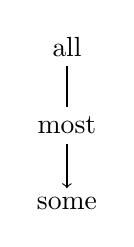
\begin{tikzpicture}
		\node[] at(0, 0) (A) {all};
		\node[] at(0, -1) (B) {most};
		\node[] at(0, -2) (C) {some};
		\draw[->] (A) -- (B) -- (C);
	\end{tikzpicture}
	\caption[]{Directed graph induced by $\vDash$ on $\lbrace \textit{all}, \textit{some}\rbrace$}\label{fig7:entailment-graph-scalar2}
\end{figure}

When compared to the simpler diagram given in Figure \ref{fig7:entailment-graph-scalar1}, this above diagram does not change the ancestors and descendants shared between \textit{all} and \textit{some}. So these two alternatives still have same granularity given this diagram. However, \textit{most} and \textit{all} have one common descendant, \textit{some}, and are not equidistant from this descendant, so have different granularities. Likewise, \textit{most} and \textit{some} have one common ancestor, \textit{all}, and are not equidistant from this ancestor, so have different granularities too. Therefore, given the diagram in Figure \ref{fig7:entailment-graph-scalar2}, \textit{some} and \textit{all} have same granularity, and this granularity differs from that of \textit{most}.



\begin{figure}[H]
	\centering
	\begin{subfigure}[b]{.45\linewidth}
		\centering
		\begin{forest}
			[CS[$\neg\exists$][\fbox{$\exists$}]]
		\end{forest}
		\caption[]{``Polar''.}\label{fig7:qtree-some-polar-r}
	\end{subfigure}
	\hfill
	\begin{subfigure}[b]{.45\linewidth}
		\centering
		\begin{forest}
			[CS[$\neg\exists$][\fbox{$\exists\wedge\neg\forall$}][\fbox{$\forall$}]]
		\end{forest}
		\caption[]{``\textit{Wh}''.}\label{fig7:qtree-some-wh-r}
	\end{subfigure}
	\caption[]{Qtrees evoked by $S_{\s}$ = \textit{Jo read some of the books}. }\label{fig7:qtrees-some-r}
\end{figure}


\begin{figure}[H]
	\centering
	\begin{subfigure}[b]{.45\linewidth}
		\centering
		\begin{forest}
			[CS[$\neg\forall$][\fbox{$\forall$}]]
		\end{forest}
		\caption[]{``Polar''.}\label{fig7:qtree-all-polar-rr}
	\end{subfigure}
	\hfill
	\begin{subfigure}[b]{.45\linewidth}
		\centering
		\begin{forest}
			[CS[$\neg\exists$][$\exists\wedge\neg\forall$][\fbox{$\forall$}]]
		\end{forest}
		\caption[]{``\textit{Wh}''.}\label{fig7:qtree-all-wh-rrr}
	\end{subfigure}
	\begin{subfigure}[b]{.45\linewidth}
		\centering
		\begin{forest}
			[CS[$\neg M$ [$\neg\exists$]][$M$][$\exists\wedge\neg\forall$][\fbox{$\forall$}]]
		\end{forest}
		\caption[]{``\textit{Wh}-articulated''.}\label{fig7:qtree-all-wh-rrr}
	\end{subfigure}
	\caption[]{Qtrees evoked by $S_{\splus}$ = \textit{Jo read all of the books}. }\label{fig7:qtrees-all-rr}
\end{figure}


\section{Appendix}
Assuming strict conditionals (UPDATE)
\begin{exe}
	\ex{\textit{exh}($\lbrace\neg\s, \neg\splus\rbrace$, $\neg$\splus) = $\s\wedge\neg\splus$ is IW in the antecedent of (\ref{ex7:shc-sw}).\\
		We have $S[\textit{exh}(\lbrace\neg\s, \neg\splus\rbrace, \neg\splus)] = \textit{exh}(\lbrace\neg\s, \neg\splus\rbrace, \neg\splus) \rightarrow \s$.\\
		And we have $S[\neg\splus] = \neg\splus \rightarrow \s$.\\
		Let $S'$ be a continuation of $S$ after \textit{exh}($\lbrace\neg\s, \neg\splus\rbrace$, $\neg$\splus). Then $S'[x]$ must have the form $x \rightarrow \r$, with $\r$ derived from the replacement of $\s$ in $S$.\\ $\textit{exh}(\lbrace\s, \splus\rbrace, \neg\splus)$ is globally weakening in $S'$:\\
		$S'[\textit{exh}(\lbrace\neg\s, \neg\splus\rbrace, \neg\splus)] = \textit{exh}(\lbrace\neg\s, \neg\splus\rbrace, \neg\splus) \rightarrow \r$\\
		\phantom{$S'[\textit{exh}(\lbrace\neg\s, \neg\splus\rbrace, \neg\splus)]$} $\equiv (\s\wedge\neg\splus) \rightarrow \r$\\
		\phantom{$S'[\textit{exh}(\lbrace\neg\s, \neg\splus\rbrace, \neg\splus)]$} $\equiv \neg(\s\wedge\neg\splus) \vee \r$\\
		\phantom{$S'[\textit{exh}(\lbrace\neg\s, \neg\splus\rbrace, \neg\splus)]$} $\equiv \neg(\s)\vee\splus \vee \r$\\
		\phantom{$S'[\textit{exh}(\lbrace\neg\s, \neg\splus\rbrace, \neg\splus)]$} $\Dashv \splus\vee \r \equiv \neg\splus \rightarrow \r = S'[\neg\splus]$\\
		Therefore, $\textit{exh}(\lbrace\s, \splus\rbrace, \neg\s)$ is incrementally weakening in $S$.}\label{ex7:iw-hc-sw-ant-m}
	\ex{\textit{exh}($\lbrace\s, \splus\rbrace$, \s) = $\s\wedge\neg\splus$ is IW in the consequent of (\ref{ex7:shc-sw}).\\
		We have $S[\textit{exh}(\lbrace\s, \splus\rbrace, \s)] = \neg\splus \rightarrow \textit{exh}(\lbrace\s, \splus\rbrace, \s)$, and $S[\s] = \neg\splus \rightarrow \s$. We know this because (\ref{ex7:iw-hc-sw-ant-m}) showed that the antecedent of (\ref{ex7:shc-sw}) cannot contain \textit{exh}.\\
		Let $S'$ be a continuation of $S$ after \textit{exh}($\lbrace\s, \splus\rbrace$, \s). Because $S'$ must result from the replacement of a constituent \textit{following} \textit{exh}($\lbrace\s, \splus\rbrace$, \s) in $S$, $S'$ can only be $S$. $\textit{exh}(\lbrace\s, \splus\rbrace, \s)$ is globally weakening in $S'=S$:\\
		$S'[\textit{exh}(\lbrace\s, \splus\rbrace, \s)] = \neg\splus \rightarrow \textit{exh}(\lbrace\s, \splus\rbrace, \s)$\\
		\phantom{$S'[\textit{exh}(\lbrace\s, \splus\rbrace, \s)]$}
		$\equiv \splus \vee \textit{exh}(\lbrace\s, \splus\rbrace, \s)$\\
		\phantom{$S'[\textit{exh}(\lbrace\s, \splus\rbrace, \s)]$} $\equiv \splus \vee (\s\wedge\neg\splus)$\\
		\phantom{$S'[\textit{exh}(\lbrace\s, \splus\rbrace, \s)]$} $\equiv \splus \vee\s$\\
		\phantom{$S'[\textit{exh}(\lbrace\s, \splus\rbrace, \s)]$} $\equiv \neg\splus \rightarrow\s$\\
		\phantom{$S'[\textit{exh}(\lbrace\s, \splus\rbrace, \s)]$} $\equiv S[\s]$\\
		Therefore, $\textit{exh}(\lbrace\s, \splus\rbrace, \s)$ is incrementally weakening in $S$}\label{ex7:iw-hc-sw-cons-m}
\end{exe}

update (for the other conditionals, that is predicted ok without exh and probalby with exh too)

(\ref{ex7:hc-s-ws-iw}) shows that that \textit{exh} is IW in the antecedent and the consequent of (\ref{ex7:shc-ws}), whether the conditional is seen as material or as strict. (\ref{ex7:shc-ws}) is therefore isomorphic to (\ref{ex7:hc-ws}), and so is correctly predicted to be non-SR, like (\ref{ex7:hc-ws}).

\begin{exe}
	\ex\label{ex7:hc-s-ws-iw}
	\begin{xlist}
		\ex\textit{exh} is IW in the antecedent of (\ref{ex7:shc-ws}); material case.\\ $\forall \Gamma.$ exh(\s) $\rightarrow$ $\Gamma$ $\equiv$ $\neg$(\s$\wedge$$\neg$\splus) $\vee$ $\Gamma$ $\equiv$ $\neg$\s{} $\vee$ \splus{} $\vee$ $\Gamma$ $\Dashv$ $\neg$\s{} $\vee$ $\Gamma$ $\equiv$ \s{} $\rightarrow$ $\Gamma$
		\ex\textit{exh} is IW in the antecedent of (\ref{ex7:shc-ws}); non-material case.\\ $\forall \Gamma.$ $\forall w: \text{exh}(\s)(w). \ \Gamma \equiv \forall w: \s(w) \wedge \neg\splus(w). \ \Gamma \Dashv \forall w: \s(w). \ \Gamma \equiv \s{} \rightarrow \Gamma$
		\ex\textit{exh} is IW in the consequent of (\ref{ex7:shc-ws}); material case.\\
		$\forall \Gamma.$ (\s{} $\rightarrow$ exh($\neg$\splus)) $\Gamma$ $\equiv$ ($\neg$\s{} $\vee$ ($\neg$\splus $\wedge$ \s)) $\Gamma$ $\equiv$ ($\neg$\s{} $\vee$ $\neg$\splus) $\Gamma$ $\equiv$ (\s{} $\rightarrow$ $\neg$\splus) $\Gamma$
		\ex\textit{exh} is IW in the consequent of (\ref{ex7:shc-ws}); non-material case.\\$\forall \Gamma.$ $\forall w: \s(w). \ \text{exh}(\neg\splus)(w) \equiv \forall w: \s(w). \ \neg\splus(w) \wedge \s(w) \Dashv \forall w: \s(w). \ \splus(w) \equiv \s{} \rightarrow \splus$
	\end{xlist}
\end{exe}



\newpage



\chapter*{General Conclusion}

\begin{flushright}
	\textit{J'aimerais te prendre par la main}\\
	\textit{M'enfuir avec toi au soleil}\\
	\textit{Sans avoir peur du lendemain}\\
	\textit{Te regarder devenir vieille}\\\vspace{2mm}
	Sexy Sushi, Retour de Bâton
\end{flushright}

The central claim of this dissertation, was that pragmatic (in)felicity is tightly related to the questions an assertive sentence attempts to answer, even implicitly. In a nutshell, a good sentence must be a good answer to a good question. Although this general idea has been entertained in the literature for a long time, earlier models of the QuD were not equipped with the tools to encode fundamental concepts such as specificity, structure-dependency, and compositionality, in precise and systematic ways. By defining (implicit) QuDs as ways to recursively and compositionally partition the Context Set, this dissertation hopefully constitutes a way forward in addressing this conceptual lacuna. Beyond the conceptual advantages of the model laid out here, we saw through a variety of examples, that this model, along with constraints on its outputs, is in fact \textit{needed} to capture challenging oddness contrasts in disjunctions, conditionals, and combinations thereof. Even beyond logical operators, we sketched how a compositional (and incremental) model of questions could interact with other familiar pragmatic devices, in particular presuppositions and constraints on their use. This makes way for broader applications of a QuD-driven model of oddness, for instance, in the domain of quantification and modality (e.g., free choice phenomena), plurality, but also phenomena like anaphora, which have been associated with presuppositions.